% Retoca las líneas marcadas con TODO según las necesidades

\documentclass[oneside,a4paper,12pt]{book} % TODO: cambia "oneside" por "twoside" a la hora de imprimirlo

\usepackage[spanish]{babel}
\usepackage[utf8]{inputenc}
\usepackage{geometry}
\usepackage{makeidx}
\usepackage{url}
\usepackage{graphicx}
\usepackage{color}
\usepackage{caption}
\usepackage{acronym}
\usepackage{hyphenat}
\usepackage{a4wide}
\usepackage[normalsize]{subfigure}
\usepackage{float}
\usepackage{titlesec}
\usepackage{multirow}
\usepackage{tabularx}
\usepackage{array}
\usepackage[Lenny]{fncychap}
\usepackage{listings} % para poder hacer uso de "listings" propios (p.ej. códigos)
\usepackage{eurosym} % para poder usar el símbolo del euro con \euro {xx}
\usepackage{hyperref} % TODO: añade la opción hidelinks para imprimirlo (los enlaces no aparecerán resaltados)

% Para que no parta las palabras
%pretolerance=10000

\newcommand{\bigrule}{\titlerule[0.5mm]} \titleformat{\chapter}[display] % cambiamos el formato de los capítulos
{\bfseries\Huge} % por defecto se usaron caracteres de tamaño huge en negrita
{% contenido de la etiqueta 
\titlerule % línea horizontal 
\filright % texto alineado a la derecha 
\Large\chaptertitlename\ % capítulo e índice en tamaño large
\Large % en lugar de 
\Huge \Large\thechapter} 
{0mm} % espacio mínimo entre etiqueta y cuerpo
{\filright} % texto del cuerpo alineado a la derecha
[\vspace{0.5mm} \bigrule] % después del cuerpo, dejar espacio vertical y trazar línea horizontal gruesa
\geometry{a4paper, left=3.5cm, right=2cm, top=3cm, bottom=2cm, headsep=1.5cm}

% Estilos para ilustrar códigos:
\definecolor{code_green}{rgb}{0,0.6,0}
\definecolor{code_gray}{rgb}{0.5,0.5,0.5}
\definecolor{code_mauve}{rgb}{0.58,0,0.82}

\lstset{frame=tb,
  language=C,
  aboveskip=3mm,
  belowskip=3mm,
  showstringspaces=false,
  columns=flexible,
  basicstyle={\small\ttfamily},
  numbers=none,
  numberstyle=\tiny\color{code_gray},
  keywordstyle=\color{blue},
  commentstyle=\color{code_green},
  stringstyle=\color{code_mauve},
  breaklines=true,
  breakatwhitespace=true,
  tabsize=3
}

\lstset{frame=tb,
  language=C++,
  aboveskip=3mm,
  belowskip=3mm,
  showstringspaces=false,
  columns=flexible,
  basicstyle={\small\ttfamily},
  numbers=none,
  numberstyle=\tiny\color{code_gray},
  keywordstyle=\color{blue},
  commentstyle=\color{code_green},
  stringstyle=\color{code_mauve},
  breaklines=true,
  breakatwhitespace=true,
  tabsize=3
}

\lstset{frame=tb,
  language=Python,
  aboveskip=3mm,
  belowskip=3mm,
  showstringspaces=false,
  columns=flexible,
  basicstyle={\small\ttfamily},
  numbers=none,
  numberstyle=\tiny\color{code_gray},
  keywordstyle=\color{blue},
  commentstyle=\color{code_green},
  stringstyle=\color{code_mauve},
  breaklines=true,
  breakatwhitespace=true,
  tabsize=3
}

% Definición de mis propios tipos: Códigos, Ecuaciones y Tablas
\DeclareCaptionType{code}[Código][Listado de códigos]
\DeclareCaptionType{myequation}[Ecuación][Listado de ecuaciones]

% TODO: especifica las reglas de separación que consideres. Algunos ejemplos:
\hyphenation{fuer-tes}
\hyphenation{mul-ti-ca-pa}
\hyphenation{res-pues-ta}
\hyphenation{di-fe-ren-tes}
\hyphenation{de-sa-rro-lla-dos}
\hyphenation{re-pre-sen-tan-do}

 % archivo de configuraci�n de estilo

\makeindex

\begin{document}
\baselineskip 1.35\baselineskip

\frontmatter

\thispagestyle{empty}
\vspace{2cm}

\begin{figure}[htb]
  \centerline{\resizebox{.60\textwidth}{!}{
\includegraphics{figs/logo_urjc}}}
\end{figure}

\begin{center}
  {\Large {\bf GRADO EN INGENIERÍA DE TECNOLOGÍAS INDUSTRIALES}}
  \vspace{5mm}
 
  {\large {Escuela Superior de Ciencias Experimentales y Tecnología}}
  \vspace{5mm}

  {\large {Curso académico 2023-2024}}

  \vspace{1cm}

  {\large {\bf Trabajo Fin de Grado}}

  \vspace{2cm}

  {\Large {Escribe el título del trabajo aquí\\
               con la segunda línea aquí\\[1cm] }}

  \vspace{5cm}
  {\bf Tutor}: Julio Vega Pérez \\
  {\bf Autor}: David Campoamor Medrano
\end{center}

\clearpage
\thispagestyle{empty}


% Este diseño se corresponde con la licencia CC-BY-NC-SA.
% Por supuesto, puedes poner la licencia que mejor se adapte al propósito de tu trabajo.
% Recuerda que, si no se especifica ninguna licencia, esta -como cualquier creación artística- pasaría a estar licenciada con todos los derechos reservados (copyright).


\thispagestyle{empty}
\begin{center}
    
\includegraphics[width=0.45\textwidth]{figs/logo_urjc.jpg}\\[1cm]

    {\large{\textbf{Grado en Ingeniería de Tecnologías Industriales}}}\\[1cm]
    {\large{\textbf{Trabajo de Fin de Grado}}}\\[1cm]
\end{center}


El presente trabajo, titulado \textit{\textbf{SISTEMA DE RECOLECCIÓN ROBÓTICO DE FRESAS MADURAS POR VISIÓN ARTIFICIAL}}, constituye la memoria correspondiente a la asignatura Trabajo de Fin de Grado que presenta D./D\textsuperscript{a}. \textit{\textbf{DAVID CAMPOAMOR MEDRANO}} como parte de su formación para aspirar al Título de Graduado/a en Ingeniería de Tecnologías Industriales. Este trabajo ha sido realizado en la \textit{\textbf{ESCUELA DE INGENIERÍA DE FUENLABRADA}} en el \textit{\textbf{DEPARTAMENTO DE TEORÍA DE LA SEÑAL Y COMUNICACIONES Y SISTEMAS TELEMÁTICOS Y COMPUTACIÓN}} bajo la dirección de \textit{\textbf{JULIO VEGA PÉREZ}}.\\[3cm]

\begin{flushright}
Móstoles, 26 de mayo de 2025
\end{flushright}

\cleardoublepage

\begin{figure}
 \ \ \ \ 
\includegraphics[width=0.25\linewidth]{figs/by-nc-sa.png}
 \label{fig:cc} 
 \end{figure}

\

\

\

\noindent
Este trabajo se distribuye bajo los términos de la licencia internacional \href{http://creativecommons.org/licenses/by-nc-sa/4.0/}{CC BY-NC-SA International License} (Creative Commons AttributionNonCommercial-ShareAlike 4.0). Usted es libre de \textit{(a) compartir}: copiar y redistribuir el material en cualquier medio o formato; y \textit{(b) adaptar}: remezclar, transformar y crear a partir del material. El licenciador no puede revocar estas libertades mientras cumpla con los términos de la licencia:

\begin{itemize}
\item \textit{Atribución}. Usted debe dar crédito de manera adecuada, brindar un enlace a la licencia, e indicar si se han realizado cambios. Puede hacerlo en cualquier forma razonable, pero no de forma tal que sugiera que usted o su uso tienen el apoyo de la licenciante.
\item \textit{No comercial}. Usted no puede hacer uso del material con propósitos comerciales.
\item \textit{Compartir igual}. Si remezcla, transforma o crea a partir del material, debe distribuir su contribución bajo la la misma licencia del original.
\end{itemize}

\begin{flushright}
		\vspace{7.0 cm}
		\emph{Documento de} \textbf{David Campoamor Medrano}. % TODO: pon aquí tu nombre cuando hagas el documento
\end{flushright}



\cleardoublepage

\chapter*{Agradecimientos}

Nunca es tarea fácil agradecer a tantas personas el apoyo, la ayuda y los consejos que han contribuido en mi beneficio, tanto personal como académico, durante todos estos años.\\

En primer lugar, me gustaría dar las gracias tanto a la Universidad Rey Juan Carlos como a todos los profesores de los que he tenido el privilegio de ser alumno, por haber sido capaces de transmitir la dedicación, pasión, disciplina y el esfuerzo tan imprescindible como necesarios para la praxis de una profesión como lo es la de ingeniero, y más concretamente en mi caso, la de ingeniero industrial.\\
Quisiera expresar mi gratitud a mi tutor, Julio Vega, por guiarme, acompañarme y ayudarme durante estos meses de trabajo, para mí fue todo un honor saber que finalmente había aceptado dirigir este trabajo final de grado, y de este modo cerrar un bonito círculo que empezó con él como profesor mío de informática en el colegio, donde nos enseñó, entre otras muchas cosas, que más allá de los editores de texto convencionales, existen otros sistemas para la preparación de documentos, por esto, este trabajo también es en parte suyo, ya que tanto estas líneas como el resto del documento están basados en sus enseñanzas.\\

Asimismo, me gustaría agradecer a Robotplus, por cumplimentar mi formación académica y darme mi primera oportunidad laboral en el ámbito industrial, y más concretamente a mis compañeros del departamento de servicio técnico y a los del departamento de I+D+i, ya que gracias a ellos hoy por hoy he podido entender y experimentar más en profundidad muchos de los principios teóricos y de los problemas que únicamente conocía sobre el papel, pudiendo desarrollarme de una manera más completa como profesional.\\

Agradecer también a mis amigos y compañeros de clase, los \textit{Hijos de la Ingeniería} y David, por no haber dejado que me rindiera incluso en los peores momentos y con todo en contra, y por haber sido un gran apoyo tanto dentro como fuera de la universidad. 
A mis amigos del equipo de baloncesto en Alcorcón, en especial a Rober y a Adri, por haber confiado siempre en que este momento llegaría, antes o después, y haber formado parte de este proceso del que desde antes de empezar la universidad ya formaban parte, al igual que mis amigos de Móstoles del colegio, el \textit{Cártel de La Manga}.Y sobre todo, gracias a Sandra, por ser para mí el claro ejemplo de que la dedicación y el trabajo duro merecen la pena, pero más allá de todo esto, por estar a mi lado día a día y ser mi compañera de vida, sin ella no habría podido soñar con finalmente llegar hasta aquí.\\

No querría concluir los agradecimientos sin hacer partícipe a toda mi familia, y en especial a mis padres y mi hermano, la paciencia que han tenido todo este tiempo conmigo, sobre todo en época de entregas y de éxamenes, pero sobre todo y más importante, la confianza depositada en mí, que mediante palabras y gestos de apoyo incondicional han demostrado. Ha sido gracias a este amor y apoyo que solo la familia sabe darte cuando más lo necesitas, por lo que sido más fácil poder alcanzar esta meta. Gracias a mis tíos y a mis primos mayores, por hacer que me interesase en el mundo de las ciencias, y más concretamente en la ingeniería y la construcción, faceta en la que ya desde pequeño había fijado mi atención jugando con aquellos bloques fabricados en plástico ABS y de colorines, ya que sin duda, fue gracias a ellos por lo que terminé de decidir embarcarme, ya desde el colegio, en las materias que guardaban mayor similitud con estos aspectos antes que en otras, puesto que veía en ellos una referencia a seguir. Pero sobre todo, gracias a mis abuelos, que como suele decirse, deberían ser eternos. Si antes hablaba de referencias, sin duda ellos han sido el máximo exponente en esto, puesto que sin sus enseñanzas y consejos, y no solo en aspectos académicos, no podría haber llegado hasta aquí. Todos ellos siempre formarán parte de mi y estarán presentes en cada una de las tomas de decisiones importantes que tenga que llevar a cabo, en las desilusiones y en los malos ratos, pero también en la consecución de mis éxitos y logros, como es el caso, aunque algunos de ellos ya no se encuentren entre nosotros o no puedan recordarlo. Espero haber podido aprender y retener algo de la sabiduría que me habéis mostrado y trasmitido.\\

\begin{flushright}
		\emph{A todas aquellas personas que, con trabajo y esfuerzo,\\
 terminan consiguiendo todo aquello que se proponen.}\\
		\par
		\vspace{1.0 cm}
		Madrid, 26 de mayo de 2025\\ %\today
		\emph{David Campoamor Medrano}
\end{flushright}

\thispagestyle{empty}



\cleardoublepage

\chapter*{Resumen\markboth{Resumen}{Resumen}}

La robótica y la visión artifical han revolucionado numerosos sectores, incluida la agricultura, en la que, a pesar de los avances tecnológicos, la recolección manual de las frutas y verduras sigue siendo un proceso laborioso, exigente y sujeto a tareas repetitivas susceptibles de derivar en errores humanos.

Uno de los mayores desafíos en este campo es la recolección de frutas pequeñas y delicadas, como lo son en particular las fresas dada su gran variabilidad en tamaño, forma y grado de maduración; ya que requieren gran precisión y un alto consumo de tiempo y esfuerzo físico por quienes lo realizan. Es por esto que la automatización de su recolección se ha convertido en una alternativa para poder mejorar y optimizar su eficiencia, reduciendo la dependencia de la mano de obra humana mediante el uso de la robótica y la inteligencia y visión artificial para identificar, seleccionar y recoger los frutos en el momento óptimo.

El presente trabajo pretende solucionar este problema mediante el desarrollo de un sistema de visión artificial para detectar el estado de maduración de las fresas y facilitar su recolección de forma automatizada, siempre y cuando el estado de maduración de la fresa sea el adecuado, con un brazo robótico y utilizando el modelo YOLOv3 en tiempo real. Mediante el procesamiento de las imágenes capturadas por una cámara, el sistema identifica la posición y calcula la distancia de cada fresa con respecto a la cámara para poder transmitir esta información a un brazo robótico de Universal Robots a través del protocolo XML-RPC, permitiendo que el robot ejecute esta recolección de forma autónoma y precisa.

Los experimentos realizados han demostrado que el sistema puede identificar fresas maduras con alta precisión en distintas condiciones de iluminación. Además, la integración con el brazo robótico ha permitido validar la eficacia del sistema en la recolección autónoma, logrando resultados satisfactorios en términos de exactitud. Estos avances confirman la viabilidad de la propuesta y sientan las bases para futuras mejoras en rendimiento, velocidad y adaptabilidad a otros cultivos.




%\cleardoublepage

\chapter*{Abstract\markboth{Abstract}{Abstract}}

Artificial intelligence and robotics have revolutionised numerous sectors, including agriculture, where, despite technological advances, the manual harvesting of fruits and vegetables remains a labour-intensive, demanding process, prone to repetitive tasks and human error.

One of the greatest challenges in this field is the harvesting of small and delicate fruits, such as strawberries, which exhibit high variability in size, shape, and ripeness level. These fruits require great precision and significant physical effort and time from those who harvest them. For this reason, the automation of harvesting has become an alternative to enhance and optimise efficiency, reducing dependence on human labour through the use of robotics and artificial intelligence and vision to identify, select, and harvest the fruits at the optimal moment.

This project aims to address this problem by developing a computer vision system capable of detecting the ripeness stage of strawberries and facilitating their automated harvesting, provided that the fruit is at the appropriate stage. The system employs a robotic arm and uses the YOLOv3 model in real time. By processing images captured by a webcamera, the system identifies the position and calculates the distance of each strawberry from the camera in order to transmit this information to an Universal Robots robotic arm via XML-RPC protocol, allowing the robot to perform harvesting in an autonomous and precise manner.

The experiments conducted have demonstrated that the system can identify ripe strawberries with high accuracy under varying lighting conditions. Furthermore, integration with the robotic arm has validated the system’s effectiveness in autonomous harvesting, yielding satisfactory results in terms of precision. These advances confirm the feasibility of the proposed approach and lay the foundation for future improvements in yield, scalability, and adaptability to other crops.





%\cleardoublepage

\chapter*{Acrónimos\markboth{Acrónimos}{Acrónimos}}

% Añade a continuación los acrónimos que uses en el documento. Algunos ejemplos:
\begin{acronym}
        \acro{ABB}{\emph{Asea Brown Boveri}}
	\acro{AER}{\emph{Asociación Española de Robótica}}
	\acro{AERO}{\emph{Autonomous Exploration Rover}}
	\acro{AGV}{\emph{Automated Guided Vehicle}}
	\acro{AI}{\emph{Artificial Intelligence}}
	\acro{AMR}{\emph{Autonomous Mobile Robot}}
	\acro{ANN}{\emph{Artificial Neural Network}}
	\acro{API}{\emph{Application Programming Interface}}
	\acro{CMI}{\emph{Cirugía Mínimamente Invasiva}}
	\acro{DLR}{\emph{Deutsches Zentrum für Luft - und Raumfahrt e.V.}}
	\acro{EKF}{\emph{Extended Kalman Filter}}
	\acro{EPFL}{\emph{Escuela Politécnica Federal de Lausana}}
	\acro{FDA}{\emph{Food and Drug Administration}}
	\acro{FOA}{\emph{Focus of Attention}}
	\acro{GA}{\emph{Genetic Algorithm}}
	\acro{GPIO}{\emph{General Purpose Input/Output}}
	\acro{GPS}{\emph{Global Positioning System}}
	\acro{HCI}{\emph{Human-Computer Interaction}}
	\acro{HRI}{\emph{Human-Robot Interaction}}
	\acro{IA}{\emph{Inteligencia Artificial}}
	\acro{IBM}{\emph{International Business Machines}}
	\acro{IFR}{\emph{International Federation of Robots}}
	\acro{ISO}{\emph{Internacional Organization for Standardization}}
	\acro{LWR}{\emph{Lightweight Robot}}
	\acro{OSRF}{\emph{Open Source Robotics Foundation}}
	\acro{PUMA}{\emph{Programmable Universal Machine for Assembly}}
	\acro{ROS}{\emph{Robot Operating System}}
	\acro{ROS-I}{\emph{Robot Operating System-Industrial}}
	\acro{SAIL}{\emph{Stanford Artificial Intelligence Laboratory}}
	\acro{SCARA}{\emph{Selective Compliance Assembly Robot Arm}}
	\acro{SRI}{\emph{Stanford Research Institute}}
	\acro{TC}{\emph{Technical Committee}}
	\acro{UR}{\emph{Universal Robots}}
\end{acronym}


\cleardoublepage

\tableofcontents

\listoffigures

\listofcodes

\listofmyequations

\listoftables

%\pagestyle{empty}

\cleardoublepage

 % aqu� se cargan todas las "primeras p�ginas"

% Bibliograf�a
\let\OLDthebibliography=\thebibliography
\def\thebibliography#1{\OLDthebibliography{#1}
  \addcontentsline{toc}{chapter}{\bibname}}

\mainmatter

\setcounter{page}{1}
\setlength{\parskip}{0.7em} % Espaciado vertical entre p�rrafos
\chapter{Introducción}
\label{cap:capitulo1}
\setcounter{page}{1}

Desde sus inicios, la robótica ha proporcionado un sinfín de posibilidades y alternativas ante problemas que anteriormente carecían de las soluciones adecuadas, pero, ¿qué es realmente la robótica?\\

Se podría definir robótica como el proceso mediante el cual una máquina intercambia energía e información con su entorno, con el propósito de alcanzar una serie de objetivos específicos. Este campo tecnológico en expansión es el resultado de décadas de colaboración continua entre biólogos, informáticos e ingenieros \cite{Koditschek21}. Dada esta multidisciplina, la robótica abarca una amplia gama de aplicaciones, desde la industria hasta la medicina, pasando por la exploración espacial, la domótica o la conducción autónoma, entre otras. Es un campo en constante evolución, impulsado por la búsqueda de soluciones innovadoras para mejorar la calidad de vida y permitir superar desafíos de manera más eficiente y segura.\\

La industria agrícola no es una excepción, ya que ha contemplado históricamente tareas que requieren una dedicación laboral considerable. No obstante, gracias a la robótica y a los sistemas de visión artificial, surge la oportunidad de transformar una serie de procesos, como puede ser la recolección de cultivos a través de la detección automatizada.\\

En las siguientes secciones se describen brevemente algunas de las aplicaciones más importantes de la robótica en la sociedad actual, así como los distintos conceptos en los cuales se basa la investigación y el desarrollo llevado a cabo para la realización de este Trabajo Fin de Grado.\\

\section{Los robots y la robótica}
\label{sec:robótica} % etiqueta para luego referenciar esta sección

Según la \textit{Federación Internacional de Robots} (IFR) se define robot según el vocabulario establecido por la \textit{International Organization for Standardization} (ISO), y esto es como \textit{mecanismo accionado programado con cierto grado de autonomía para realizar tareas de locomoción, manipulación o posicionamiento} \cite{ISO8373}.\\  

El término robot fue utilizado por primera vez por Karel Capek en su obra de teatro \textit{Rossum’s Universal Robots}, publicada en 1920. Esta palabra viene del vocablo checo \textit{robota} que significa trabajo, en el sentido de la obligatoriedad, entendido como servidumbre, trabajo forzado o esclavitud \cite{Sanchez07a}. Aunque esta definición es un punto de partida, es cierto que es posible diferir en aspectos como si un robot debe controlarse automáticamente o podría ser autónomo o si un robot debe ser reprogramable. A un nivel más amplio, cualquier máquina que pueda utilizarse para llevar a cabo acciones o tareas complejas de forma automática puede considerarse un robot \cite{Raj19}.\\

Históricamente, las civilizaciones antiguas, como la egipcia y la griega, dieron los primeros pasos en lo que se puede denominar robótica clásica, construyendo autómatas y mecanismos diseñados para imitar acciones humanas, con características mecánicas rudimentarias. 
Con el paso del tiempo, la ciencia y la ingeniería avanzaron, y los conceptos de la robótica comenzaron a tomar forma más definida hasta que, en el siglo XX, con el desarrollo de la ingeniería en sus diferentes ramas (mecánica, electrónica, informática, telecomunicaciones), Isaac Asimov (1920-1992) utilizó por primera vez el término robótica y postuló las tres leyes de la robótica en su libro \textit{I Robot}, publicado en 1950, coincidiendo con el apogeo de la robótica moderna. Asimov consideró necesario añadir una cuarta ley, antepuesta a las demás, la número cero, que afirma que un robot no debe actuar simplemente para satisfacer intereses individuales, sino que sus acciones deben preservar el beneficio común de toda la humanidad \cite{Sanchez07b}.\\

%Es también en 1950 cuando Alan Mathison Turing publica \textit{Computing Machinery and Intelligence} y propone una prueba en forma de entidad matemática abstracta, test o máquina de Touring, que demuestra la existencia de problemas computacionales irresolubles que ninguna máquina es capaz de solventar. Se puede afirmar que un programa de ordenador no llegará nunca a ser tan inteligente como un ser humano y que un robot no podrá suplir al ser humano de forma completa \cite{Sanchez07b}, preocupación que históricamente ha atenuado el entusiasmo en torno a las nuevas tecnologías \cite{Mokyr15}.\\

Partiendo de todos estos avances y del interés por automatizar las tareas de producción, la robótica va adquiriendo un gran desarrollo \cite{Sanchez07b}. Es debido a este desarrollo que, atendiendo al propósito y al contexto en el que se utilicen estos robots, se fueron creando varios grupos en función de los que clasificarlos. Estos tres grandes grupos fueron, en función de una serie de criterios generales: robots industriales, robots de servicio y robots médicos.

\subsection{Robots industriales}
\label{sec:robots_industriales}

Se define robot industrial como un manipulador polivalente, reprogramable y controlado automáticamente, programable en tres o más ejes, que puede ser fijo o móvil para su uso en aplicaciones de automatización industrial \cite{ISO8373}.\\

%El inicio de la robótica industrial puede datarse en la década de 1950, aunque algunos tipos de automatización en el entorno industrial empezaron a aparecer desde los tiempos de la Revolución Industrial. 
La evolución de los robots industriales puede subdividirse en cuatro categorías: las tres primeras abarcan el período comprendido entre los años cincuenta y finales de los noventa, mientras que la cuarta generación abarca desde 2000 hasta nuestros días \cite{Gasparetto19}.\\

La primera generación, o primeros manipuladores (1950-1967), eran básicamente máquinas programables que no tenían comunicación con el entorno externo y con algoritmos de control sencillos (punto a punto). En cuanto al hardware, contaban con equipos de baja tecnología, sin servo-controladores. Sin embargo, en 1954, George Devol y Joseph Engelberger formaron la empresa Unimation, empresa que desarrollaría Unimate (ver en Figura \ref{fig:primer_robot_industrial}), considerado el primer robot industrial de la historia, fabricado en 1961 \cite{Zamalloa17}.
  
  \begin{figure}[H]
    \begin{center}
      \subcapcentertrue
      \subfigure[Joseph Engelberger y George Devol]{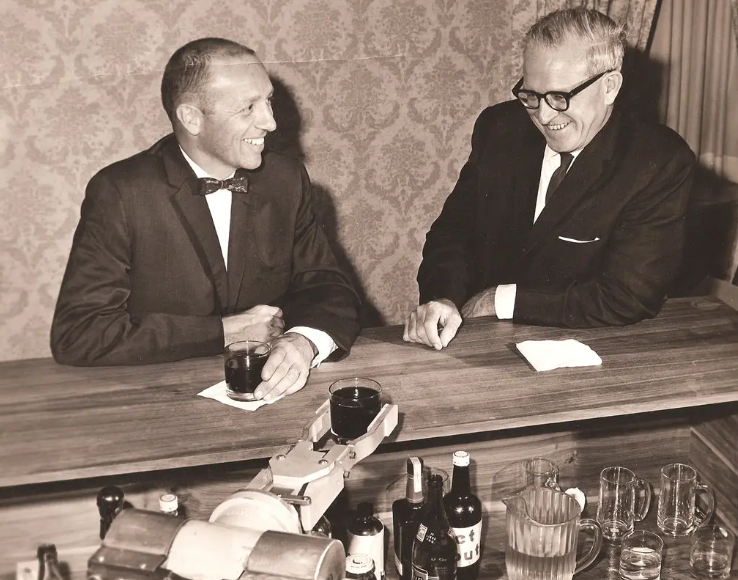
\includegraphics[width=62mm]{figs/Engelberger_Devol.png}}
      \hspace{2mm}
      \subfigure[Robot Unimate]{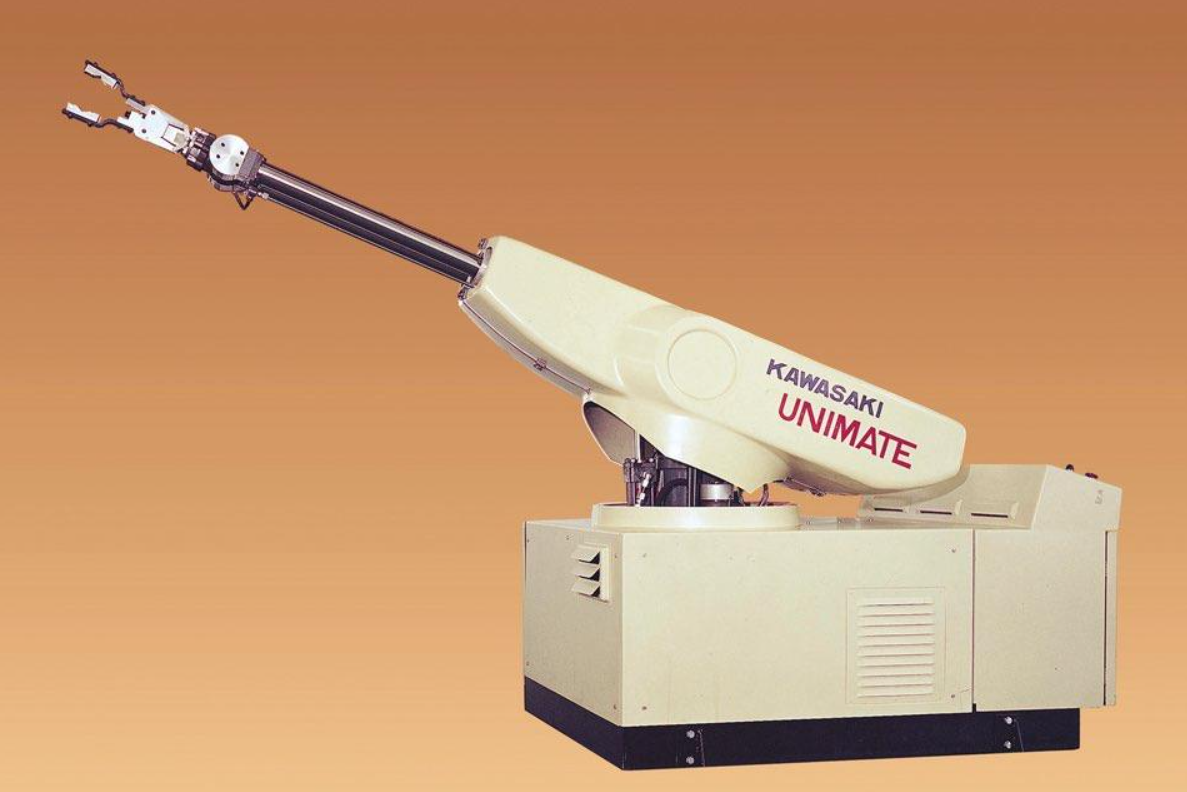
\includegraphics[width=73mm]{figs/Unimate robot.png}}
    \end{center}
    \caption{Primer robot industrial}
    \label{fig:primer_robot_industrial}
  \end{figure}
  
%Empresas como Ford y General Motors empezaron a plantearse la automatización de sus plantas productivas, por lo que, en 1962, la empresa AMF Corporation fabricó un nuevo robot llamado Versatan, un robot cilíndrico que Ford encargó para sus fábricas. Este robot, fue también el primero que se instaló en un centro productivo en Japón \cite{Gasparetto19}. \\

La segunda generación, o robots sensorizados (1968-1977), eran máquinas programables básicas con posibilidades limitadas de comportamiento autoadaptativo y capacidades elementales para reconocer el entorno externo, poseían sistemas sensoriales avanzados y eran robots de gran volumen que se utilizaban principalmente en automoción \cite{Zamalloa17}. \\

En 1968, en el Stanford Artificial Intelligence Laboratory (SAIL) se confecciona el WAVE, el primer lenguaje de programación para robots. En 1969, %Unimation concedió a Kawasaki Heavy Industries Ltd. la licencia para producir robots para el mercado japonés y asiático, conduciendo al desarrollo del Kawasaki-Unimate 2000, el primer robot industrial construido en Japón. Es también en este año cuando 
Víctor Scheinman, un estudiante de ingeniería mecánica de la Universidad de Standford, diseñó y construyó el primer prototipo de brazo robótico (Figura \ref{fig:standford_arm}), cuya cinemática inversa podía resolverse de manera analíticamente cerrada, permitiendo una rápida ejecución de la trayectoria \cite{Gasparetto19}. \\

  \begin{figure}[H]
    \begin{center}
      \subcapcentertrue
      \subfigure[Victor Scheinman con el Standford Arm]{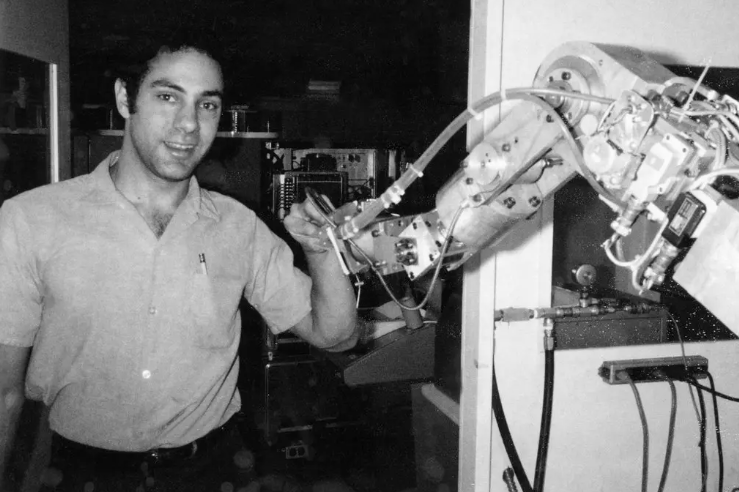
\includegraphics[width=62mm]{figs/Victor_Scheinman.png}}
      \hspace{2mm}
      \subfigure[Standford Arm]{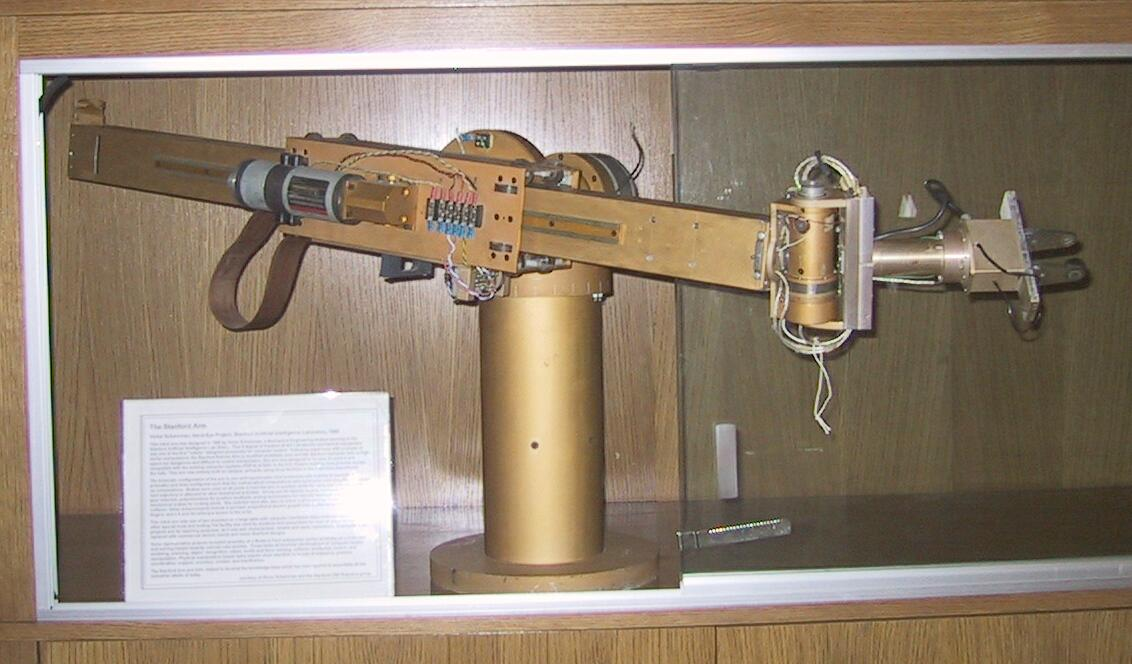
\includegraphics[width=71mm]{figs/Standford_arm.jpeg}}
    \end{center}
    \caption{Standford Arm}
    \label{fig:standford_arm}
  \end{figure}
 
%En 1969, el ingeniero de la compañía Yaskawa, T Mori, acuña el término mecatrónica, que integra el conjunto de mecanismos de control automático imprescindibles para el desarrollo de cualquier máquina inteligente \cite{Sanchez07b} tal y como muestra el diagrama de la Figura \ref{fig:Mecatrónica}.
  
  %\begin{figure} [h!]
   % \begin{center}
   %   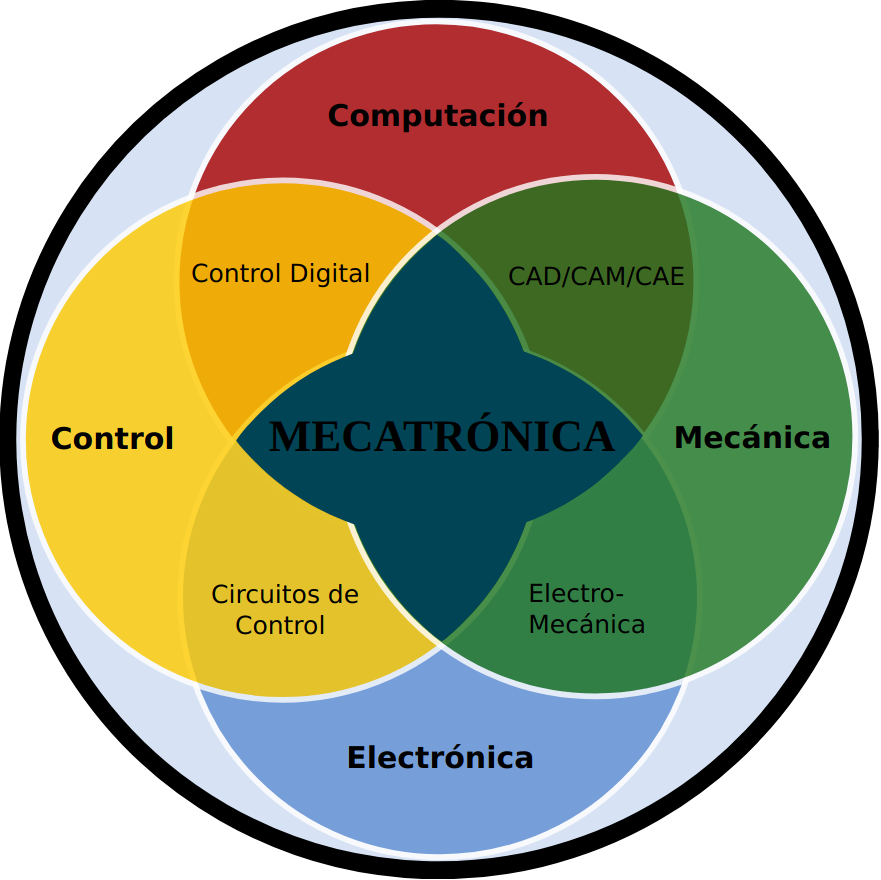
\includegraphics[width=65mm]{figs/meca.png}
   % \end{center}
   % \caption{Diagrama mecatrónico de construcción de máquinas inteligentes}
   % \label{fig:Mecatrónica}
  %\end{figure}
  
En 1973, KUKA\footnote{\url{https://www.kuka.com/es-es}} construyó el primer robot industrial con 6 ejes electromecánicos llamado Famulus. Un año más tarde, Cincinnati Milacron introdujo en el mercado el robot T3 (Figura \ref{fig:T3}). Cincinnati Milacron (adquirida por ABB\footnote{\url{https://new.abb.com/products/robotics}} en 1990). El robot T3 fue el primer robot comercial controlado por un microordenador \cite{Zamalloa17}.\\
  
  \begin{figure} [H]
    \begin{center}
      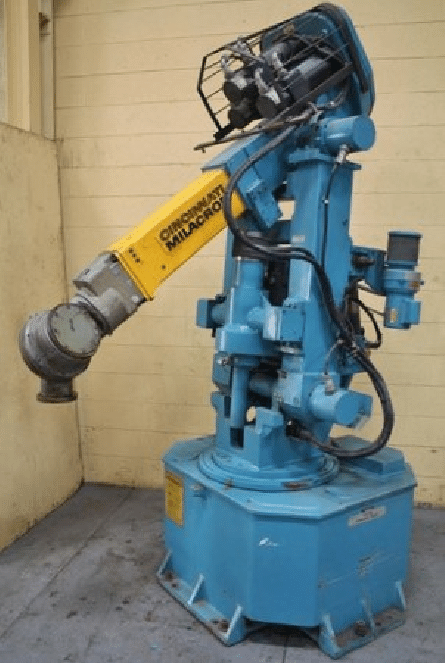
\includegraphics[width=55mm]{figs/T3_robot.png}
    \end{center}
    \caption{Robot Cincinnati Milacron T3}
    \label{fig:T3}
  \end{figure}
  
La tercera generación, o robots industriales (1978-1999), disponían de controladores específicos (ordenadores), siendo un punto clave en la caracterización de esta generación, además del surgimiento de nuevos lenguajes de programación para el control de los robots, la posibilidad de reprogramarlos y la inclusión parcial de la visión artificial \cite{Zamalloa17}.\\ %A finales de los años setenta y principios de los ochenta, otros avances científicos y técnicos contribuyeron a la difusión de los robots \cite{Gasparetto19}, que junto a que las empresas de todo el mundo invirtieron miles de millones de dólares en del mundo para automatizar tareas básicas en sus cadenas de montaje, supusieron que los robots poblaran muchos sectores industriales para automatizar una amplia variedad de actividades \cite{Zamalloa17}.\\ 
En 1978, Unimation diseñó y fabricó el robot PUMA. El PUMA (\textit{Programmable Universal Machine for Assembly}) fue considerado durante muchas décadas el arquetipo de los robots antropomórficos \cite{Gasparetto19}. Ese mismo año, el científico japonés Hiroshi Makino, de la Universidad de Yamanashi, propuso una nueva estructura cinemática. El robot con esta estructura se denominó SCARA (\textit{Selective Compliance Assembly Robot Arm})(ver Figura \ref{fig:Scara}), ya que su conformidad en la dirección horizontal resultó menor que la conformidad en la dirección vertical. Por esta razón, así como por la ligereza de la cadena cinemática (que permitía un controlador más sencillo y rápido), este robot era adecuado para ser empleado en tareas como el ensamblaje de objetos pequeños \cite{Makino80}.
  
  \begin{figure} [H]
    \begin{center}
      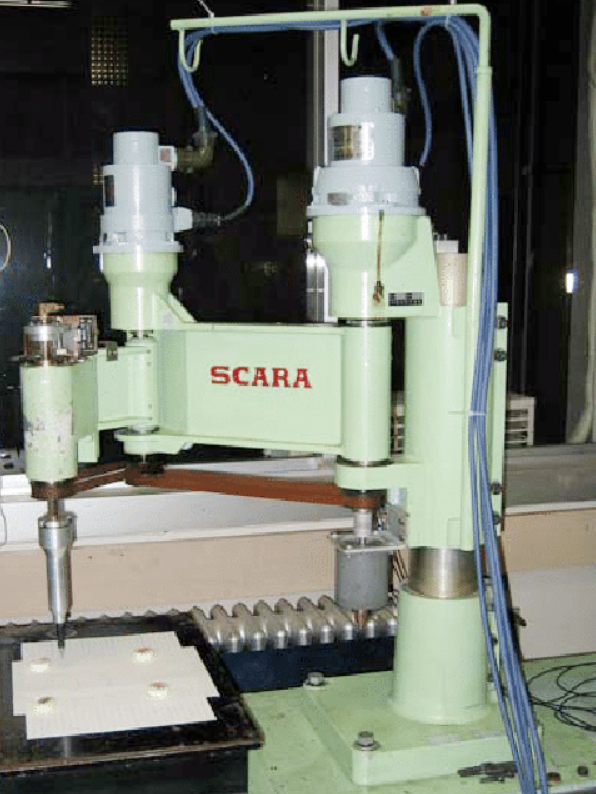
\includegraphics[width=45mm]{figs/Scara.png}
    \end{center}
    \caption{Uno de los primeros prototipos de robot SCARA}
    \label{fig:Scara}
  \end{figure}
  
%Más tarde, en 1981, en la Universidad Carnegie-Mellon se desarrolló un robot de impulsión directa que utiliza motores eléctricos en las articulaciones, evitando la distorsión de las transmisiones mecánicas convencionales. En 1982, IBM introduce el robot de montaje industrial RS-1 que utiliza un brazo constituido por 3 dispositivos de deslizamiento \cite{Sanchez07b}. De la idea de emplear cadenas cinemáticas paralelas en lugar de las clásicas cadenas cinemáticas en serie, junto con la de crear un robot ligero capaz de moverse a gran velocidad, surgió el arquetipo del robot Delta (que apareció en 1992), concebido por el científico suizo Reymond Clavel en la Escuela Politécnica Federal de Lausana (EPFL) \cite{Clavel91}. En comparación con los robots en serie, los robots paralelos tienen un espacio de trabajo más pequeño, pero pueden funcionar a una velocidad mucho mayor, siendo la arquitectura cinemática ideal para los robots dedicados a operaciones de pick-and-place de alta velocidad. 
Basado en este tipo de estructura, ABB desarrolló el Flex-Picker (Figura \ref{fig:Flexpicker_ABB}) en 1998, siendo este el robot de picking más rápido del mundo \cite{Gasparetto19}.\\
  
  \begin{figure} [H]
    \begin{center}
      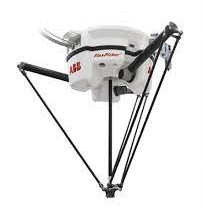
\includegraphics[width=45mm]{figs/flexpicker_ABB.jpeg}
    \end{center}
    \caption{Robot ABB IRB 360 Flexpicker}
    \label{fig:Flexpicker_ABB}
  \end{figure}
  
A partir del año 2000, aparece la cuarta generación o robots inteligentes (2000-Actualidad), que se caracteriza por la inclusión de capacidades informáticas avanzadas, ya que los ordenadores no sólo trabajan con datos, si no también pueden realizar razonamientos lógicos y aprender, puesto que la Inteligencia Artificial comienza a ser incluida parcial y experimentalmente en estos robots. Los sensores son más sofisticados, y envían información al controlador y la analizan mediante estrategias de control complejas para que el robot pueda basar sus acciones en información sólida y fiable. Es en esta generación cuando se introducen los robots colaborativos \cite{Zamalloa17}.\\
\pagebreak
  
Los requisitos de velocidad y peso de un robot han dado lugar a novedosos diseños cinemáticos y de transmisión. Desde el principio, la reducción de la masa y la inercia de las estructuras robóticas ha sido un objetivo primordial en el desarrollo de la robótica. El brazo humano, con una relación peso-carga de 1:1, se consideraba la referencia definitiva \cite{Siciliano16}. %Con este objetivo se desarrollaron, gracias a la colaboración entre la empresa alemana KUKA y el Instituto de Robótica y Mecatrónica del Centro Aeroespacial Alemán (DLR), tres generaciones de robots ligeros, permitiendo a investigadores e ingenieros desarrollar nuevas aplicaciones de robótica industrial y de servicios con un rendimiento sin precedentes. 
En el año 2004, con motivo de Automática, la mayor exposición de robots del mundo, se presentó por primera vez la combinación entre el robot ligero del DLR y la controladora KUKA, denominado RoboAssistant, donde se permitió a los visitantes mover y programar manualmente el robot, haciendo la visión de un robot que asiste a un trabajador durante los procesos de producción evidente para los visitantes \cite{Bischoff10}. \\
  
  
Es en estos procesos de producción, donde la manipulación a dos manos puede ser crítica para tareas de ensamblaje complejas, manipulación simultánea
y procesamiento de piezas de trabajo o para la manipulación de objetos de gran tamaño, por lo que en 2005, MOTOMAN presenta el primer robot comercial para la manipulación sincronizada a dos manos \cite{Siciliano16} (ver Figura \ref{fig:MOTOMAN}).\\

  \begin{figure} [H]
    \begin{center}
      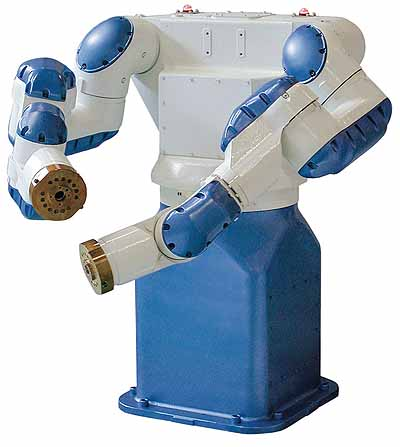
\includegraphics[width=55mm]{figs/MOTOMAN.jpg}
    \end{center}
    \caption{Robot Motoman DA-20}
    \label{fig:MOTOMAN}
  \end{figure}
  
Sin embargo, fue en el año 2006 %cuando, tras haber estado trabajando en la búsqueda de vías para el desarrollo en serie del robot LWR3 del DLR, y tras una intensa cooperación entre KUKA y el DLR para transmitir a los desarrolladores de KUKA los conocimientos necesarios para para el desarrollo de brazos ligeros, componentes y electrónica integrada, 
cuando se toma la decisión de producir una primera pequeña serie del robot ligero del KUKA LWR3 \cite{Bischoff10}, tal y como muestra la Figura \ref{fig:Lightweight Robot (LWR)}.
  
  \begin{figure}[H]
    \begin{center}
      \subcapcentertrue
      \subfigure[RoboAssistant en Automatica 2004]{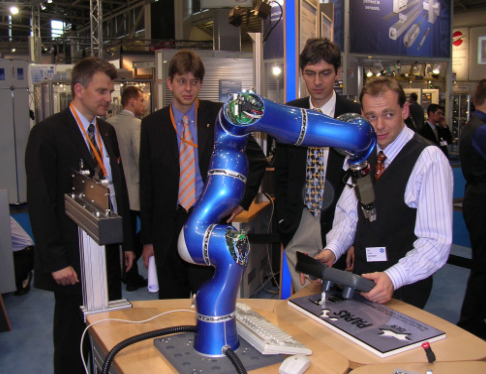
\includegraphics[width=72mm]{figs/RoboAssistant.png}}
      \hspace{2mm}
      \subfigure[Robot KUKA LWR3 con controladora (2006)]{\includegraphics[width=55mm]{figs/Kuka_lightweightrobot_2006.png}}
    \end{center}
    \caption{LWR3}
    \label{fig:Lightweight Robot (LWR)}
  \end{figure}
  
A principios de 2007, dos estudiantes de doctorado de la Universidad de Standford, Keenan Wyrobek y Eric Bergerlas, pusieron las primeras piezas de lo que eventualmente se convertiría en ROS (Robot Operating System). Uno de los preceptos principales que se tuvo en cuenta para la creación de este sistema operativo para robots fue el de crear un sistema que permitiese al máximo posible la reutilización de código, dando soporte a distintos tipos de robots y de aplicaciones. Esto resultó en la incorporación de ROS en una sorprendentemente amplia variedad de robots, extendiéndose incluso a dominios más allá de la comunidad académica de investigación a la que se dirigió inicialmente. Los años siguientes superaron todas las expectativas debido a que los avances en el ámbito de la robótica se compartieron de manera reproducible en ROS, y la Open Source Robotics Foundation (OSRF) se convirtió en el administrador principal de ROS en 2014. Con el objetivo de atender de manera más efectiva las demandas de una comunidad ROS más extensa y abordar sus nuevos escenarios de aplicación, la OSRF se dedicó a desarrollar ROS2 como un conjunto de paquetes paralelos que pudieran ser instalados junto a ROS1 (la versión original de ROS que nació en el año 2010, Figura \ref{fig:PR_ROS}) y ser compatibles entre sí. %Además, la popularidad de ROS ha seguido creciendo en la industria con el apoyo de proyectos como ROS-Industrial (ROS-I), una iniciativa de código abierto que extiende las capacidades avanzadas de ROS a hardware y aplicaciones industriales relevantes. \cite{Suarez22}.\\
  
  \begin{figure}[H]
    \begin{center}
      \subcapcentertrue
      \subfigure[Robot PR1]{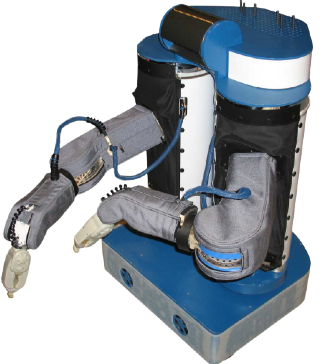
\includegraphics[width=52mm]{figs/PR1.png}}
      \hspace{2mm}
      \subfigure[Robot PR2]{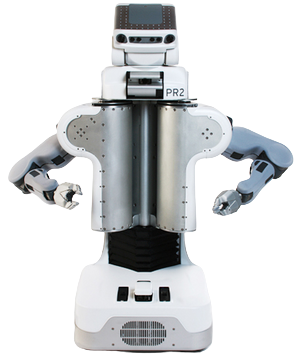
\includegraphics[width=50mm]{figs/PR2.png}}
    \end{center}
    \caption{Robots utilizados para el desarrollo de ROS}
    \label{fig:PR_ROS}
  \end{figure}
    
En el año 2008 se entrega el primer robot colaborativo o cobot, el UR5 de Universal Robots\footnote{\url{https://www.universal-robots.com/es/}} (Figura \ref{fig:UR5}), considerado como uno de los logros tecnológicos más significativos de la década en la comunidad robótica. El brazo robótico es pionero en la programación 3D fácil de usar pero sofisticada, con una interfaz de usuario intuitiva que permite a cualquier persona configurarlo y utilizarlo de forma rápida. Esta empresa, fundada en el año 2005 por Esteben Østergaard, Kasper Støy y Kristian Kassow tras conocerse en la Universidad de Dinamarca, surgió con el objetivo de hacer que la robótica sea accesible para las pequeñas y medianas empresas\footnote{\url{https://www.universal-robots.com/es/acerca-de-universal-robots/nuestra-historia/}}.\\
  
Esben H. Østergaard, Director de Tecnología y cofundador de Universal Robots, tomó el trabajo original de Peskhin y Colgate, dos investigadores de la empresa automovilística Ford de los años 90, que decidieron crear un nuevo robot industrial, más pequeño y ágil que los tradicionales, que saliera de su jaula para colaborar estrechamente con el ser humano en las tareas de calidad y personalización de los productos, sin embargo, no fueron capaces, puesto que el problema estaba en la relación entre seguridad y rendimiento, ya que el aumento de la primera reducía el de la segunda. Østergaard consiguió diseñar un sistema de seguridad y control para el cobot que lo bloquea en caso de colisión con el operario, %Como recuerda el propio Østergaard, la seguridad era la clave con la que la robótica colaborativa podía entrar en el escenario industrial. Así se creó un robot 
siendo capaz de operar en espacios confinados, en estrecho contacto con humanos, y sin instalar costosas barreras de seguridad \cite{Cusano22}.
  
  \begin{figure} [H]
    \begin{center}
      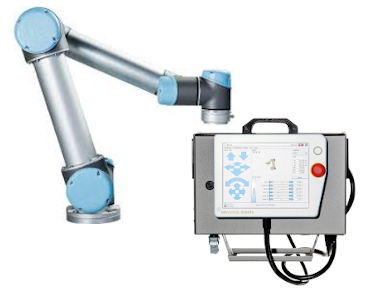
\includegraphics[width=75mm]{figs/UR5_controller.png}
    \end{center}
    \caption{UR5 con su controladora}
    \label{fig:UR5}
  \end{figure}
  
Más tarde, en 2018, Universal Robots presenta los robots colaborativos e-Series, que se pueden ver en la Figura \ref{fig:UR_e-Series}, que incluían avances tecnológicos que permitían un desarrollo más rápido para una mayor variedad de aplicaciones, ofrecía una programación más sencilla y seguía las normas de seguridad ISO más actuales y recientes\footnote{\url{https://www.universal-robots.com/es/acerca-de-universal-robots/nuestra-historia/}}.
 
  \begin{figure}[H]
    \begin{center}
      \subcapcentertrue
      \subfigure[UR presenta los  nuevos e-Series en Automatica 2018]{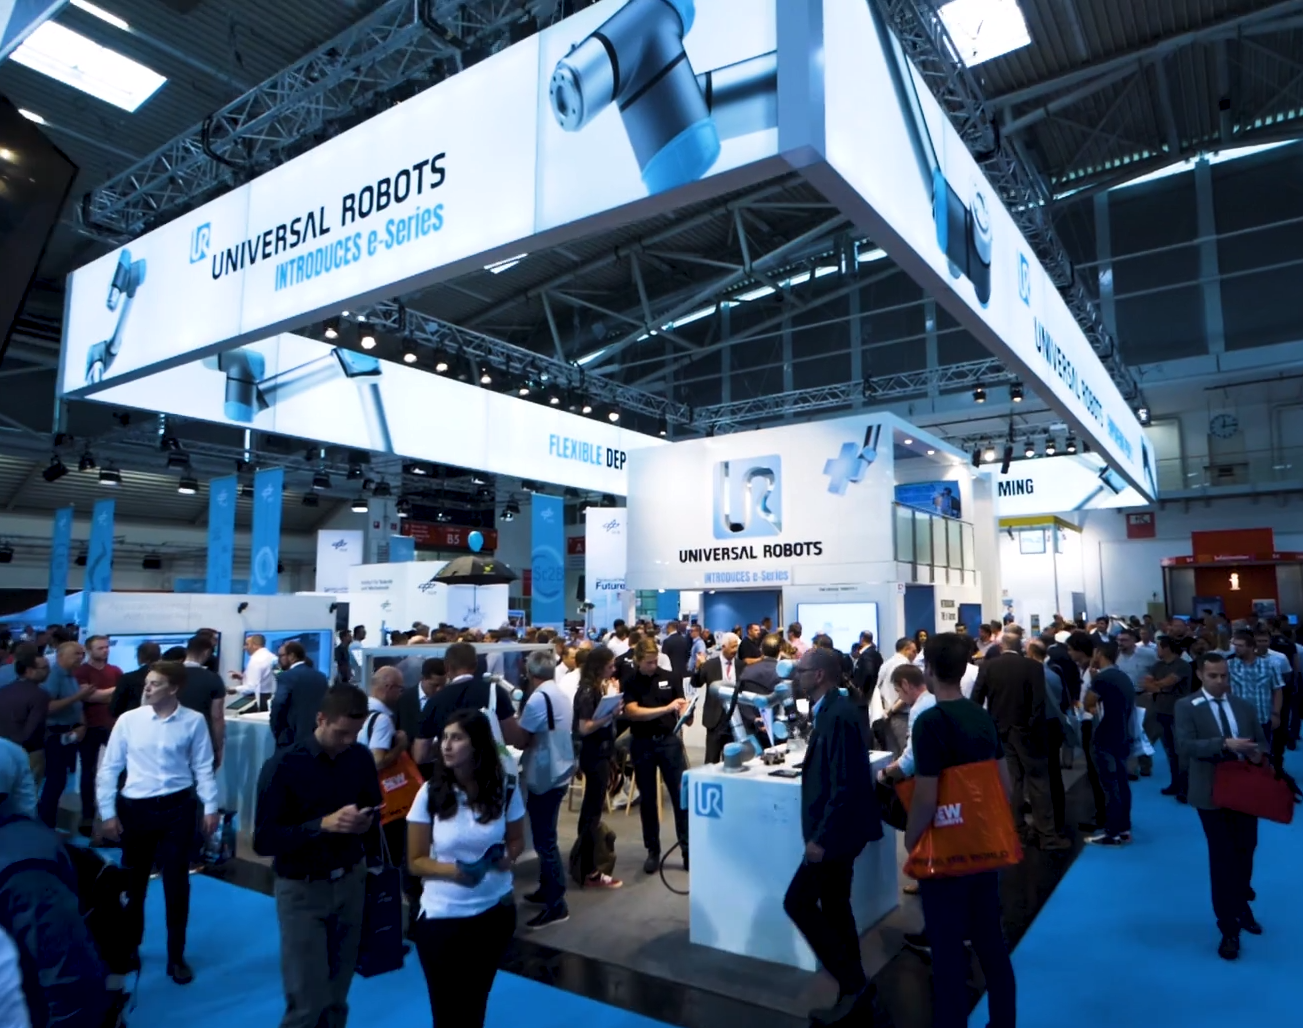
\includegraphics[width=75mm]{figs/UR Automatica 2018.png}}
      \hspace{2mm}
      \subfigure[UR e-Series]{\includegraphics[width=65mm]{figs/UR e-series.jpg}}
    \end{center}
    \caption{Universal Robots e-Series}
    \label{fig:UR_e-Series}
  \end{figure}

\pagebreak
Esta cuarta generación de robótica industrial ha establecido un sólido punto de partida para una continua revolución en el campo de la automatización. 
Es esencial destacar que varios de los modelos de robots mencionados previamente han seguido evolucionando y mejorando con el tiempo, siendo fruto de estas mejoras, la comercialización de nuevos modelos y series. 
Debido a que la tecnología se encuentra en constante desarrollo y a la colaboración cada vez más estrecha entre humanos y robots, el futuro de la robótica industrial promete seguir transformando radicalmente nuestros métodos de trabajo y producción, abriendo así nuevas oportunidades y desafiando constantemente los límites de lo que podemos lograr en la automatización industrial, así como en los otros dos grandes grupos de la robótica, como la robótica de servicio y la robótica médica.
   
\subsection{Robots de servicio}
\label{sec:robot_servicio}

Se define robot de servicio como un robot que realiza tareas útiles para las personas o los equipos, incluyendo en esta la manipulación o el servicio de artículos, el transporte, el apoyo físico, la orientación o información, el aseo personal, la cocina y la manipulación de alimentos y la limpieza en el ámbito personal; y la inspección, vigilancia, manipulación de objetos, transporte de personas, orientación o información, cocina y manipulación de alimentos y limpieza en el ámbito profesional \cite{ISO8373}.\\

%Su historia se remonta a la década de 1960, cuando surgieron los primeros intentos de crear robots para ayudar en tareas domésticas y de atención al cliente. Uno de los precursores de estos robots de servicio en 1968 fue el robot Shakey, desarrollado por el Laboratorio de Investigación de Inteligencia Artificial de Stanford (Stanford Research Institute, SRI). Shakey (ver en Figura \ref{fig:shakey}), provisto de múltiples sensores y medios para desplazarse por el suelo, además de control remoto por radio \cite{Sanchez07b}, podía realizar tareas de planificación, búsqueda de rutas y reordenación de objetos sencillos, siendo el primer robot móvil con capacidad para percibir y razonar sobre su entorno\footnote{\url{https://www.sri.com/hoi/shakey-the-robot/}}. 

%  \begin{figure} [H]
%    \begin{center}
%      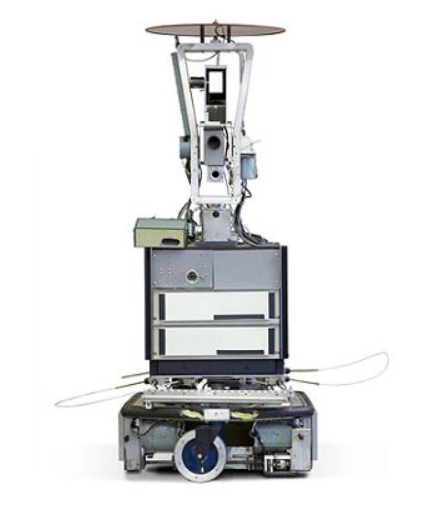
\includegraphics[width=65mm]{figs/Shakey.png}
%    \end{center}
%    \caption{Robot Shakey}
%    \label{fig:shakey}
%  \end{figure}
     
%Sin embargo, fue a mediados de los años 80 cuando en los laboratorios y centros de investigación dedicados a la robótica se trató de revitalizar la importancia de los robots en nuestra sociedad, planteando las ventajas que el uso del robot podía traer en tareas en las que el ser humano asumía riesgos o en las que las capacidades de aquel estaban limitadas por factores como la fuerza o la precisión necesaria. Fue precisamente al entenderse que estas nuevas aplicaciones de la robótica no tenían un uso industrial con el objetivo de fabricar bienes, sino que se trataba de un empleo para desarrollar tareas para las personas, cuando se catalogaron como aplicaciones en el sector servicios \cite{Barrientos02}(ver ejemplos en la Figura \ref{fig:Robots_servicio}).\\

En la práctica, las actuales y potenciales aplicaciones no industriales de los robots son tan variadas y diferentes que se dificulta su catalogación \cite{Barrientos02}; sin embargo, existen ciertas características especiales en estos robots de servicio %(ver ejemplos en la Figura \ref{fig:Robots_servicio})
que los hacen diferentes de los robots industriales \cite{Aracil08}, y los caracterizan para llevar a cabo estas tareas para las personas, siendo las principales características estos tres atributos de diseño: representación, antropomorfismo y orientación a la tarea, es decir, los robots de servicio pueden tener una representación física %(por ejemplo, Pepper) 
o tener una representación únicamente virtual %(por ejemplo, Alexa, ya que el software de IA virtual que funciona de forma autónoma y aprende con el tiempo también puede clasificarse como robot de servicio)
, diseñarse como humanoides (es decir, antropomorfos) simulando una apariencia humana o como no humanoides %(por ejemplo, el robot de limpieza Roomba de iRobot \footnote{\url{https://www.irobot.es/}} (Figura \ref{fig:roomba})
, y pueden realizar tareas analíticas %gracias a la potencia informática subyacente 
o tareas emocionales-sociales (por ejemplo, robots de recepción) \cite{Wirtz18}.\\

% \begin{figure}[H]
%    \begin{center}
%      \subcapcentertrue
%      \subfigure[Alexa]{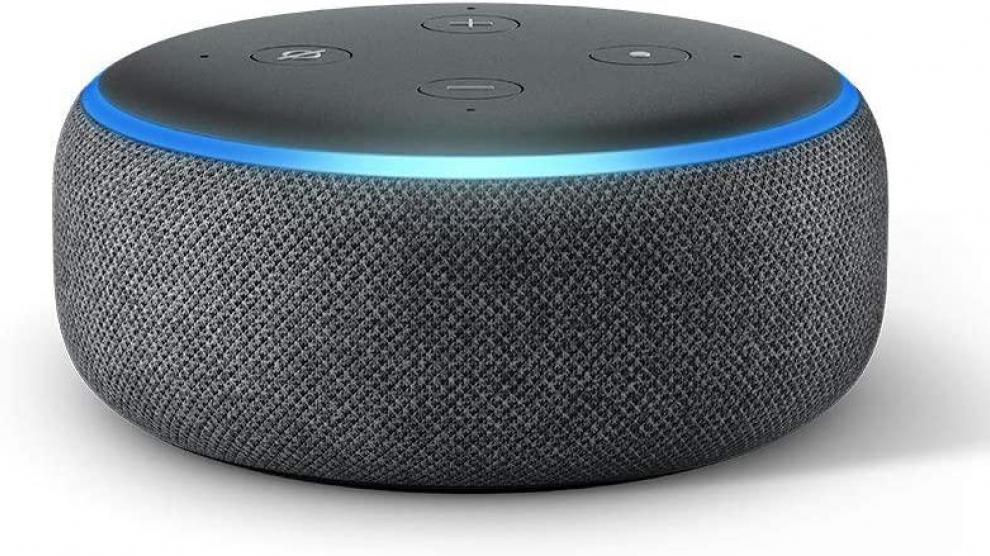
\includegraphics[width=45mm]{figs/Alexa.jpeg}}
%      \hspace{2mm}
%      \subfigure[Pepper]{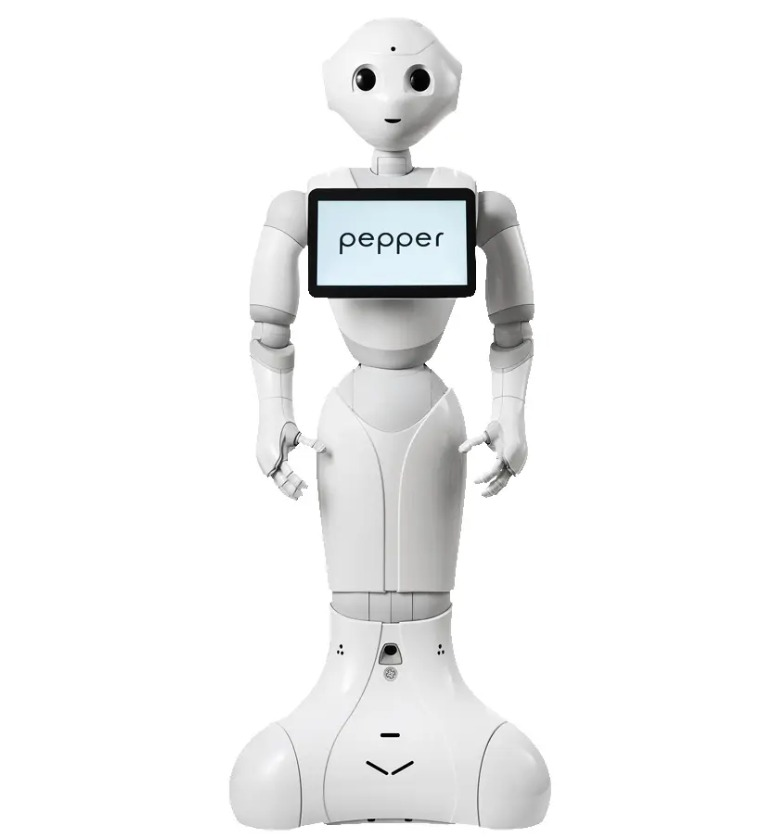
\includegraphics[width=45mm]{figs/Pepper.jpeg}}
%      \hspace{2mm}
%      \subfigure[Sophia]{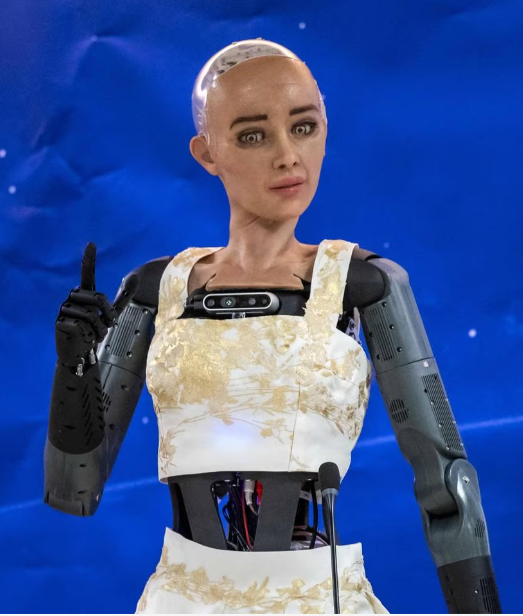
\includegraphics[width=38mm]{figs/Sophia.png}}
%    \end{center}
%    \caption{Robots de servicio}
%    \label{fig:Robots_servicio}
%  \end{figure}

Tratando de establecer una división de los robots de servicio, la norma ISO 8373:2012, así como la Federación Internacional de Robótica o IFR, propuso clasificarles en diferentes categorías según su función y aplicación en robots para uso doméstico y personal y robots de servicio destinados a un uso profesional \cite{Gonzalez21}, siendo las aplicaciones más importantes las siguientes:

\begin{itemize}
 \item \textit{Limpieza:} Suelen estar equipados con sensores y tecnología de navegación que les permite moverse de manera autónoma por el espacio, detectar obstáculos y llevar a cabo actividades de limpieza de manera eficiente. 
 
 \begin{figure} [H]
  \begin{center}
    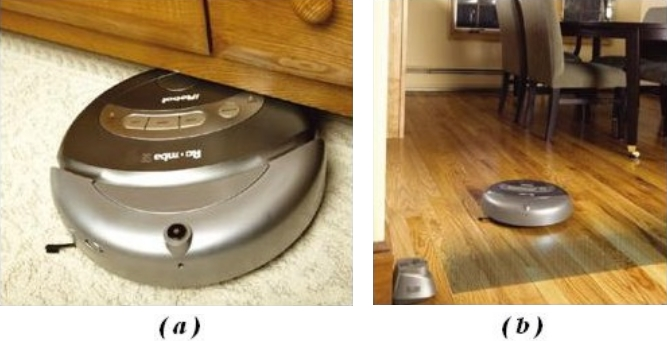
\includegraphics[width=90mm]{figs/roomba}
  \end{center}
  \caption{Robot aspirador Roomba de iRobot}
  \label{fig:roomba}
 \end{figure}
 
 \item \textit{Inspección y mantenimiento:} Son máquinas diseñadas para llevar a cabo tareas de supervisión, evaluación y mantenimiento en entornos de infraestructura o áreas de difícil acceso. Estos robots suele ser máquinas autónomas o teleoperadas equipadas con sensores, cámaras y herramientas especializadas que les permiten evaluar, reparar y mantener equipos, estructuras y sistemas en entornos desafiantes o peligrosos. 
 
 \begin{figure}[H]
    \begin{center}
      \subcapcentertrue
      \subfigure[Spot de Boston Dynamics]{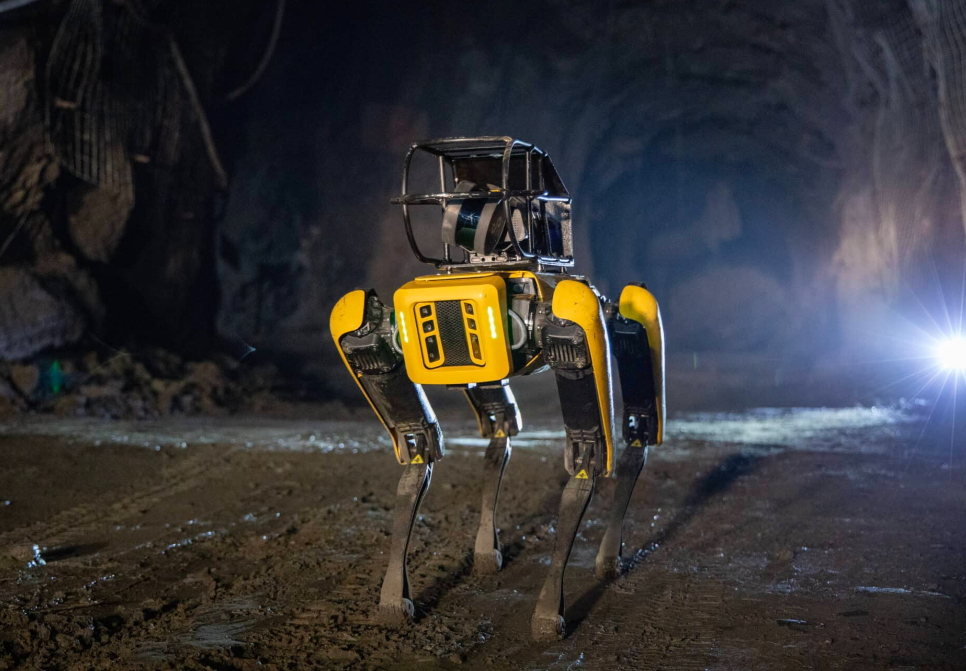
\includegraphics[width=60mm]{figs/Spot.png}}
      \hspace{2mm}
      \subfigure[ROBTET, robot para el mantenimiento de líneas de alta tensión]{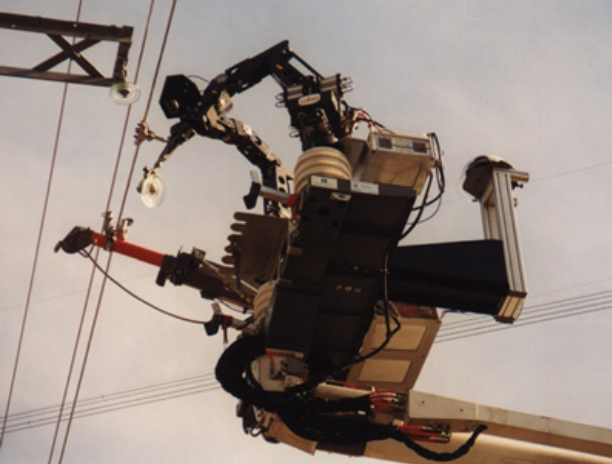
\includegraphics[width=55mm]{figs/ROBTET.png}}
    \end{center}
    \caption{Robots de inspección y mantenimiento}
    \label{fig:Robots de inspección y mantenimiento}
  \end{figure}
 
 
 \item \textit{Educación:} %Aquellos robots utilizados en educación 
Son robots diseñados para facilitar el aprendizaje y la enseñanza en los diferentes niveles educativos%. Estos robots 
, pudiendo ser utilizados en aulas, bibliotecas y entornos de aprendizaje para ayudar a los estudiantes a adquirir habilidades, fomentar la creatividad y brindar experiencias educativas interactivas.\\
 
 \begin{figure}[H]
    \begin{center}
      \subcapcentertrue
      \subfigure[Robot NAO]{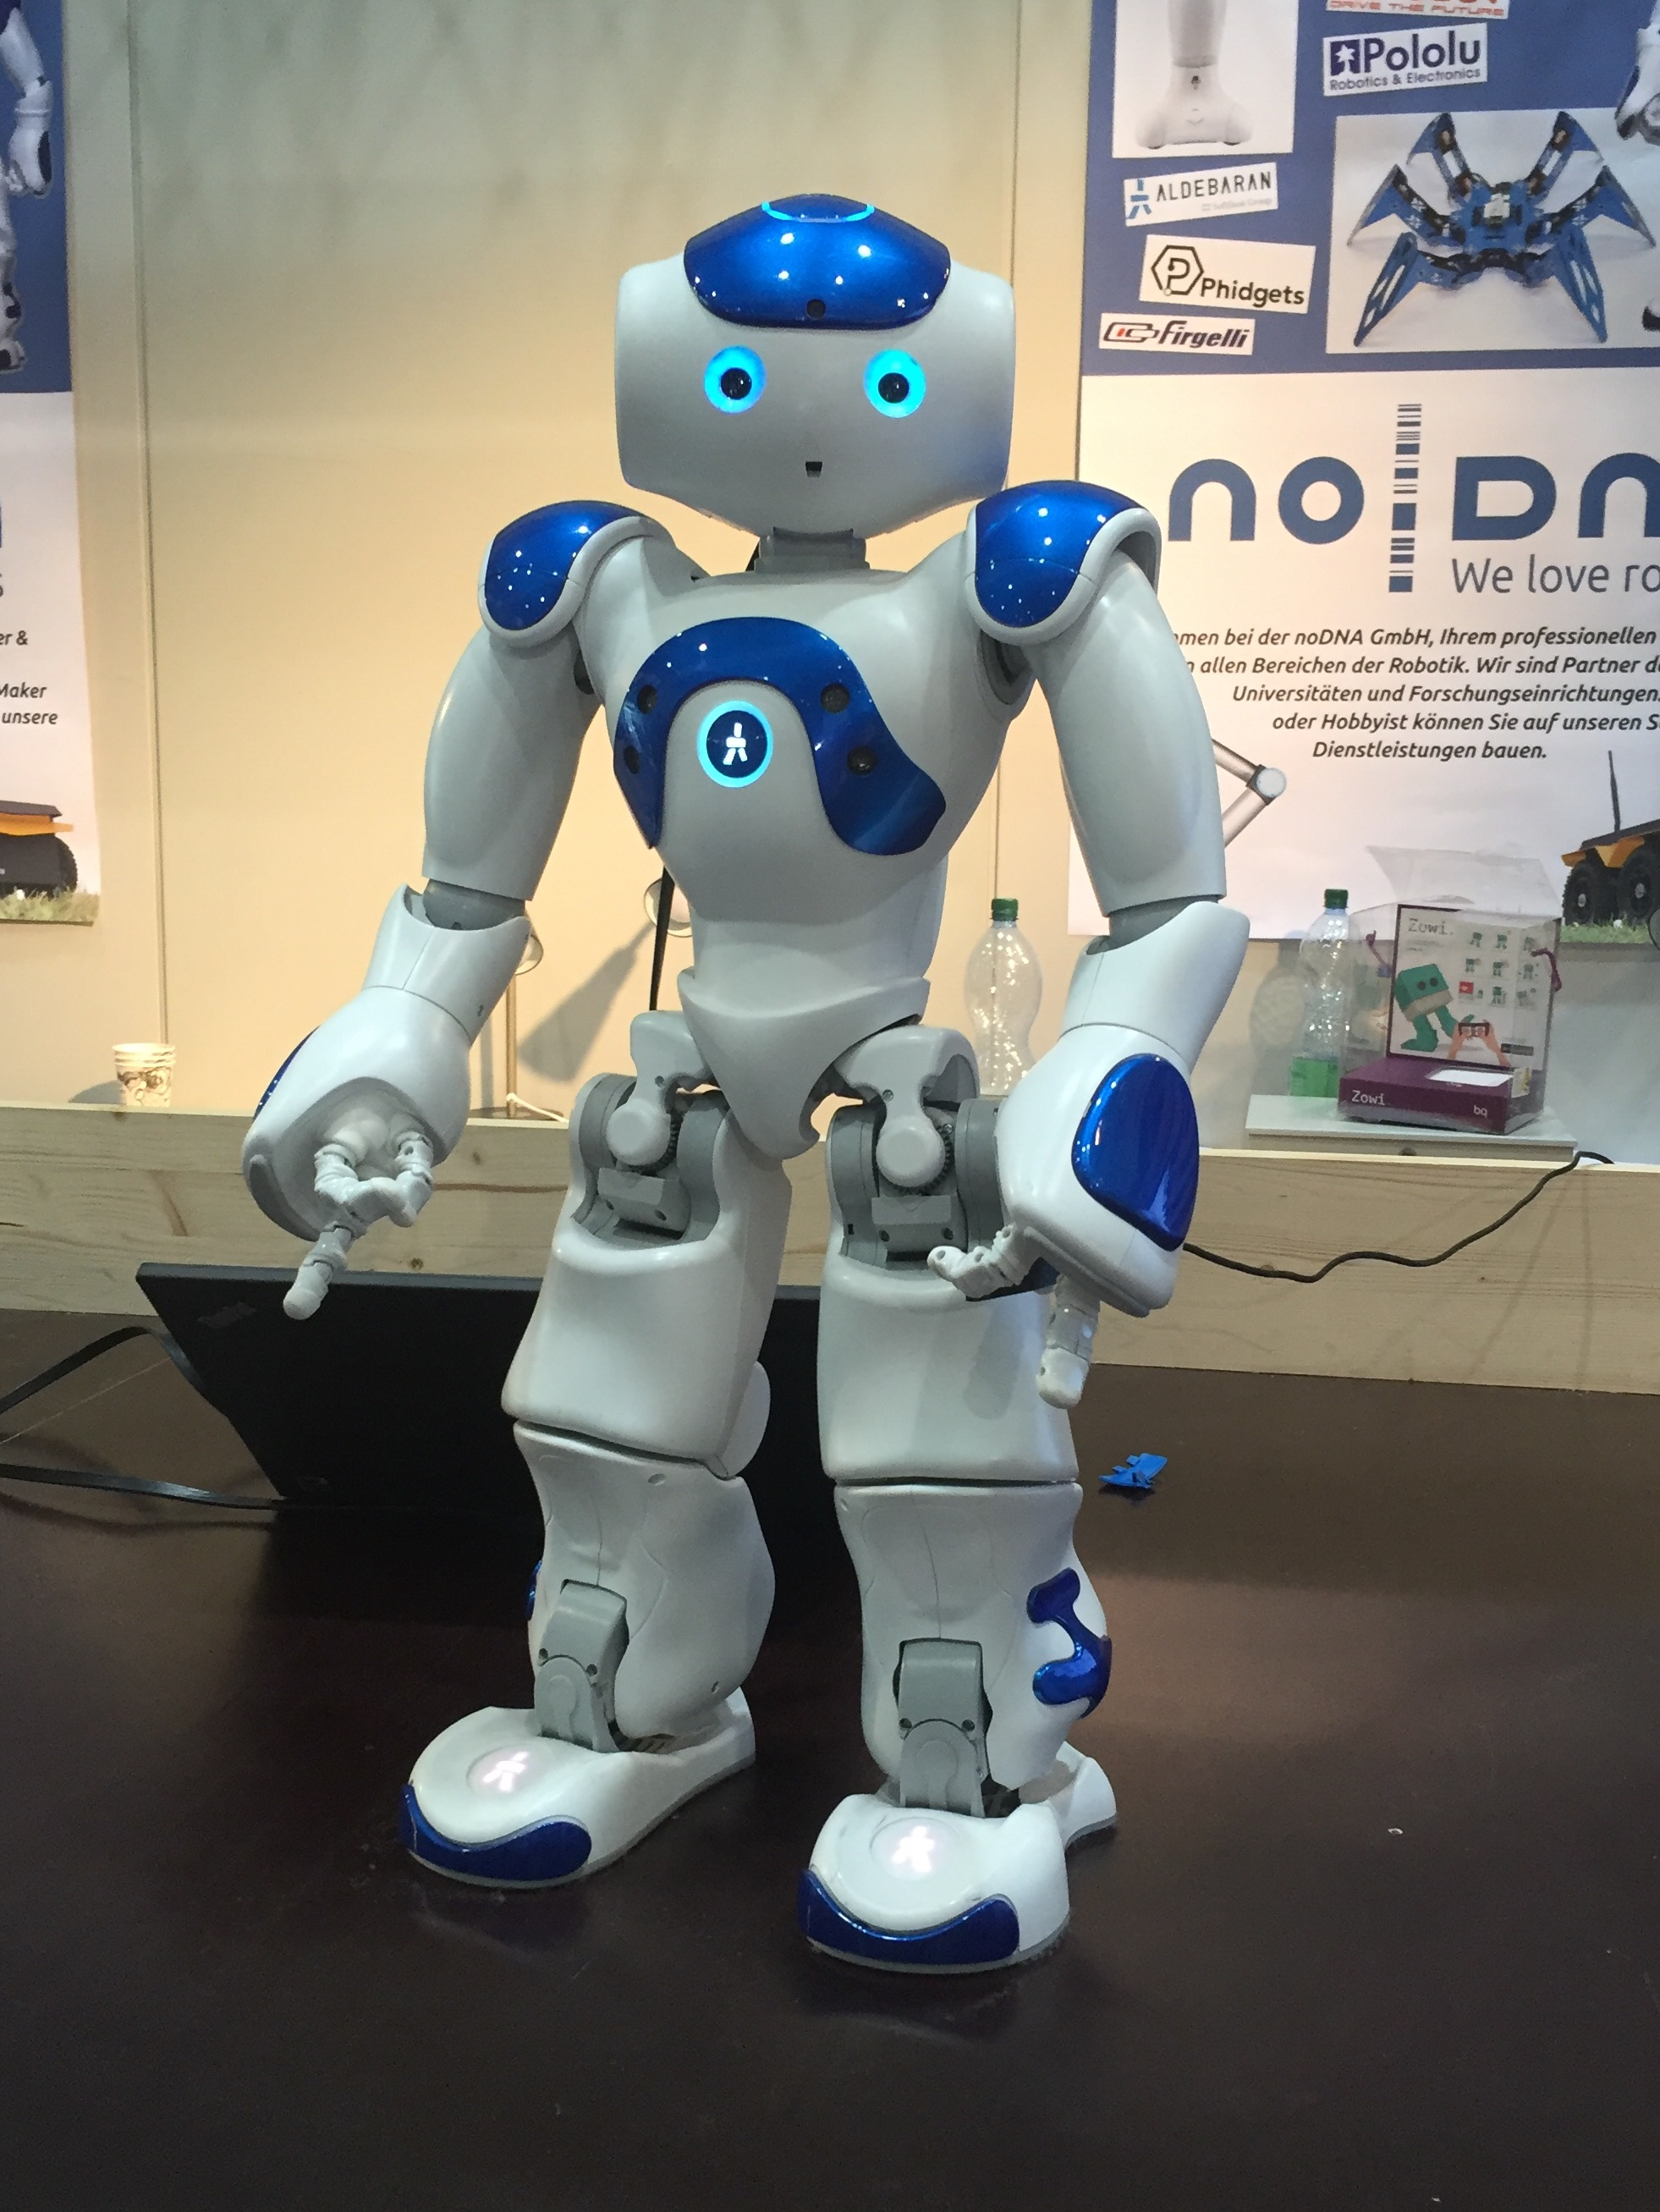
\includegraphics[width=40mm]{figs/Robot NAO.jpg}}
      \hspace{2mm}
      \subfigure[Turtlebot 4]{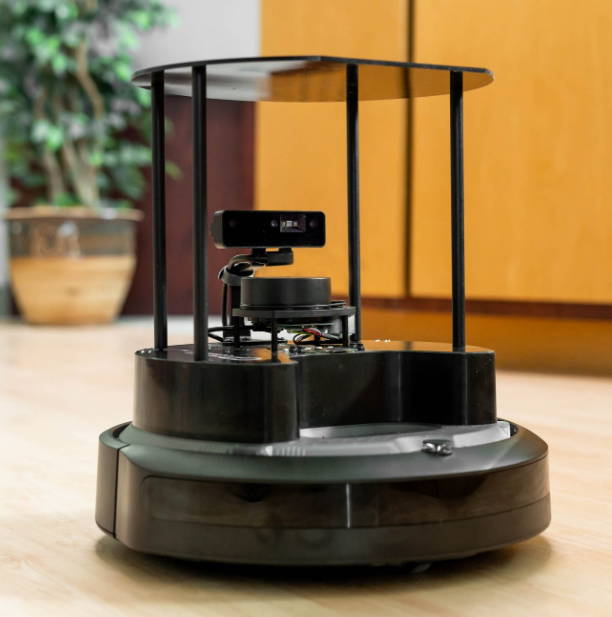
\includegraphics[width=53mm]{figs/Turtlebot 4.png}}
    \end{center}
    \caption{Robots de educación}
    \label{fig:Robots de educación}
  \end{figure}
 
 \item \textit{Logística:} Los robots de servicio utilizados en logística son robots diseñados para llevar a cabo tareas relacionadas con la gestión y el movimiento de mercancías y productos en entornos de almacenamiento, distribución y transporte. Estos robots desempeñan un papel fundamental en la optimización de la cadena de suministro, mejorando la eficiencia y la precisión en la manipulación de productos. Un ejemplo del posible uso de estos robots en el sector agrícola, es la primera granja vertical de interior del mundo en Estados Unidos, que producirá 18 millones de kilogramos de fresas al año, marcando un hito en la agricultura moderna, y demostrando que la automatización e integración de la robótica en este tipo de granjas verticales puede transformar la producción y recolección de alimentos a gran escala \cite{EcoInventos24}.
 
% \begin{figure} [H]
%  \begin{center}
%    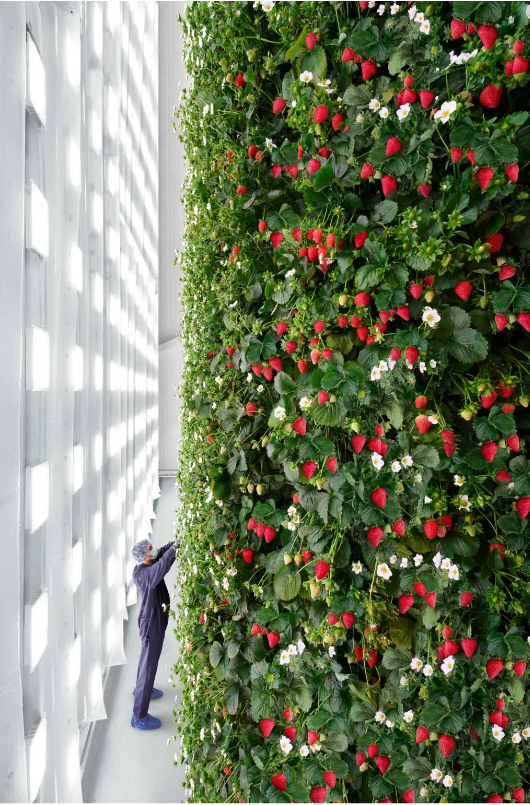
\includegraphics[width=50mm]{figs/agricultura vertical 1.png}
%  \end{center}
%  \caption{Agricultura vertical}
%  \label{fig:agricultura_vertical}
% \end{figure}
 
%Por otro lado, dentro de los robots de logística empleados para el movimiento de mercancías, se pueden distinguir dos grandes grupos: Vehículos Guiados Automáticos (AGV) y Robots Móviles Autónomos (AMR). La principal diferencia entre los AMR y los AGV radica en la capacidad de adaptación y autonomía, ya que los AMR son altamente flexibles, autónomos y versátiles, con capacidades autónomas avanzadas que les permiten ajustarse rápidamente a cambios en los entornos de trabajo, mientras que los AGV siguen rutas predefinidas y son adecuados para tareas de transporte predecibles en entornos más controlados.
 
 \begin{figure}[H]
    \begin{center}
      \subcapcentertrue
      \subfigure[AGV Robots Kiva de Amazon]{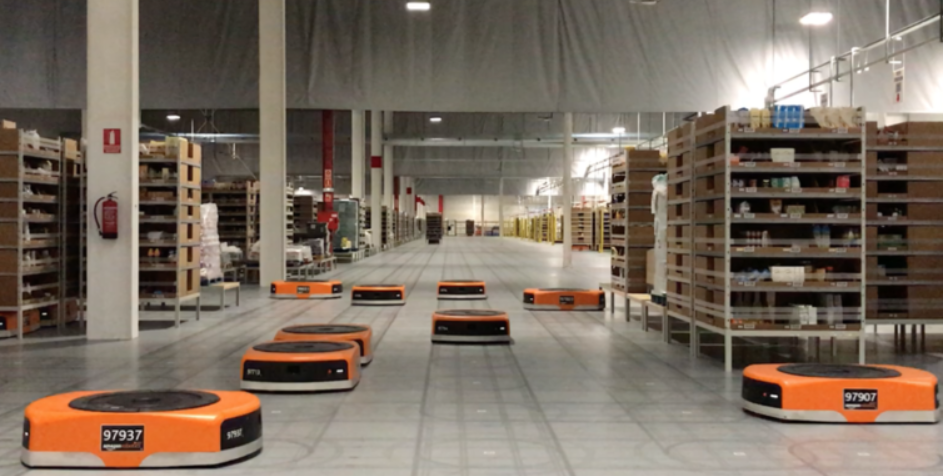
\includegraphics[width=67mm]{figs/AGV Amazon.png}}
      \hspace{2mm}
      \subfigure[AMRs de MiR]{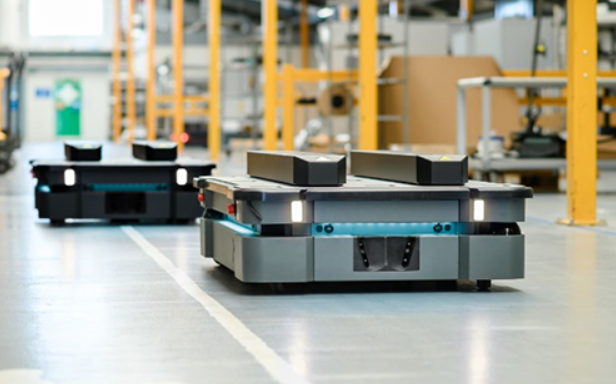
\includegraphics[width=55mm]{figs/MiR.png}}
    \end{center}
    \caption{Robots de logística}
    \label{fig:Robots de logística}
  \end{figure}
  
 \pagebreak 
 \item \textit{Entretenimiento:} Son robots diseñados específicamente para proporcionar experiencias lúdicas y de entretenimiento a las personas. Estos robots se utilizan en una variedad de contextos, siendo máquinas robóticas diseñadas para interactuar con el público. 
 
  \begin{figure}[H]
    \begin{center}
      \subcapcentertrue
      \subfigure[SONY Aibo]{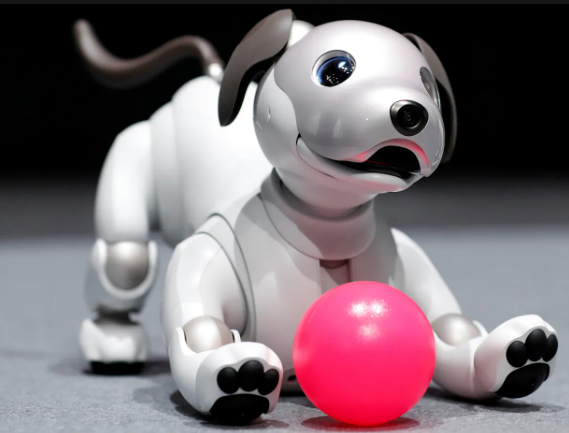
\includegraphics[width=50mm]{figs/SONY Aibo.png}}
      \hspace{2mm}
      \subfigure[Dron DJI Spark]{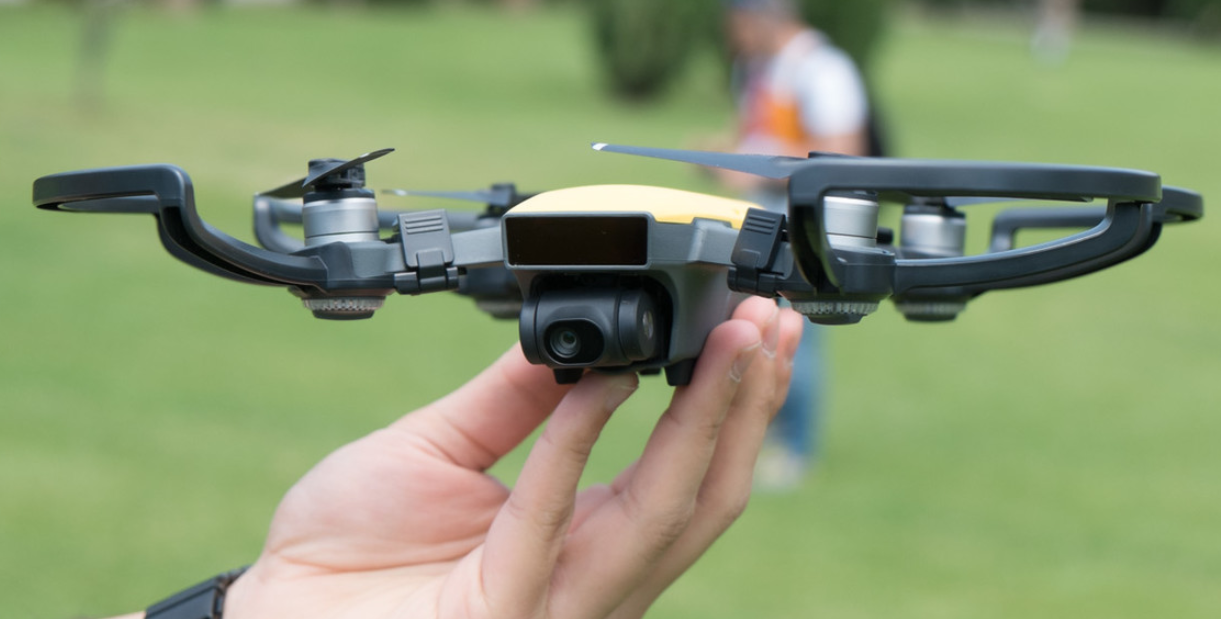
\includegraphics[width=76mm]{figs/Dron DJI Spark.png}}
    \end{center}
    \caption{Robots de entretenimiento}
    \label{fig:Robots_entretenimiento}
  \end{figure}
   
\end{itemize}

La robótica de servicio representa una revolución en la asistencia y el apoyo a diversas industrias, desde la logística hasta la atención al cliente en el comercio minorista. Sin embargo, su impacto va más allá, extendiéndose hasta la atención médica. En este contexto, la robótica médica emerge como una vanguardia tecnológica que fusiona la innovación robótica con la medicina moderna para ofrecer soluciones innovadoras en diagnóstico, tratamiento y rehabilitación, demostrando su potencial para revolucionar la forma en que brindamos y recibimos atención médica.
 
\subsection{Robots médicos}
\label{sec:robotica_industrial} 

Se define \textit{robot médico} como aquellos dispositivos electromecánicos que desempeñan parcial o totalmente algunas funciones de los seres humanos o de sus órganos al resolver problemas médicos, ayudando a mejorar la asistencia al paciente y los resultados, a la vez que aumenta la eficiencia operativa \cite{Kraevsky10}.\\

Los robots médicos se desarrollaron por primera vez hace poco más de tres décadas para permitir a los cirujanos operar a sus pacientes a distancia o con mayor precisión. A finales de los años noventa, había 2 tipos de telemanipuladores quirúrgicos aprobados por la Administración de Alimentos y Medicamentos de los Estados Unidos (FDA): el Zeus y el da Vinci (Figura \ref{fig:RobotDaVinci}), introducido en 1998-1999, que permitía aumentar la precisión de las cirugías mínimamente invasivas (CMI) \cite{Romero20}.\\

\begin{figure} [H]
    \begin{center}
      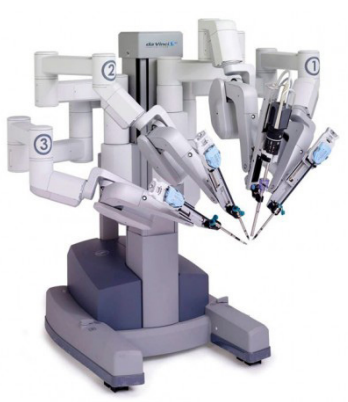
\includegraphics[width=10cm]{figs/Robot Da Vinci.png}
    \end{center}
    \caption{Robot Da Vinci}
    \label{fig:RobotDaVinci}
\end{figure}

Las primeras aplicaciones fueron en los campos de neurocirugía y cirugía ortopédica, siendo la cirugía donde mayor impacto han tenido los robots médicos, %A medida que se ha hecho patente la aceptación de los robots quirúrgicos por nuestros sistemas sanitarios, los investigadores en robótica han ido centrando cada vez más su atención en cómo podría ser la próxima generación de robots médicos. Su atención no se limita a los robots quirúrgicos, y también 
sin embargo, se están investigando otras áreas de la medicina, como los robots para realizar rehabilitación física con pacientes con discapacidades motores, como el exoesqueleto Ekso Bionics, robots de telepresencia para la interacción del paciente con el personal sanitario externo, como el robot RP-VITA, automatización de farmacias, robots para desinfectar clínicas, etc. \cite{Dupont21}\\

% \begin{figure}[H]
%    \begin{center}
%      \subcapcentertrue
%      \subfigure[Exoesqueleto Ekso Bionics]{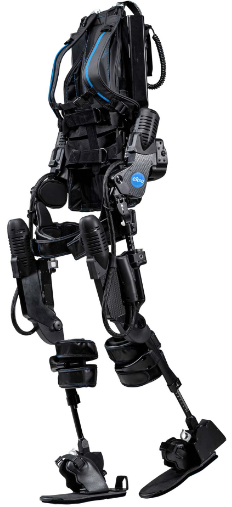
\includegraphics[width=35mm]{figs/Ekso Bionics.png}}
%      \hspace{20mm}
%      \subfigure[Robot RP-VITA]{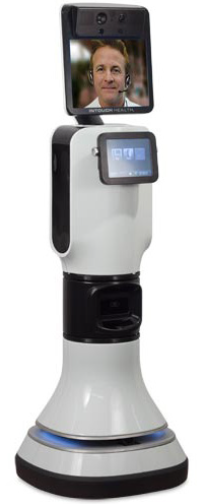
\includegraphics[width=35mm]{figs/RP Vita.png}}
%    \end{center}
%    \caption{Robots médicos}
%    \label{fig:Robots_medicos}
%  \end{figure}

El rápido crecimiento de la robótica médica se debe a una combinación de mejoras tecnológicas (motores, materiales y teoría de control), los avances en imagen médica (mayor resolución, resonancia magnética y ecografía 3D) y una mayor aceptación por cirujanos y pacientes de los procedimientos laparoscópicos y la asistencia robótica \cite{Beasley12}, convirtiéndose en un campo interdisciplinario que abarca desde cirugía asistida por robots hasta sistemas de diagnóstico de vanguardia. Gran parte de su éxito radica en la integración de tecnologías avanzadas, como la inteligencia y la visión artificial. Estas disciplinas están redefiniendo la forma en que los robots médicos pueden interactuar con el entorno, interpretar datos y, en última instancia, mejorar los resultados en la atención médica.\\

A continuación, explicaremos el impacto que la inteligencia y la visión artificial están teniendo en la robótica, y las capacidades y oportunidades que estas presentan en una inmensa variedad de aplicaciones.

\section{Inteligencia Artificial}
\label{sec:IA} 

La Inteligencia Artificial (IA) es un área multidisciplinaria de la ciencia %de gran interés por ser un área multidisciplinaria 
donde se realizan sistemas que tratan de hacer tareas y resolver problemas como lo hace un humano;así mismo, trata de simular de manera artificial las formas de pensamiento y de trabajar del cerebro para la toma de decisiones \cite{Ponce14}.\\

El origen del concepto y de los criterios de desarrollo de la IA se remontan al año 1936, con el matemático inglés Alan Turing, quien definió una máquina abstracta como ya vimos en la sección \ref{sec:robótica}, que sirvió de base de la noción de algoritmo y la definición de clase de problemas deducibles \cite{Hardy01}, y quien intuyó la importancia que jugaría el aprendizaje automático en el desarrollo de la IA al afirmar que, en lugar de intentar emular mediante una máquina la mente de un adulto, quizá sería más factible intentar emular la mente de un niño y luego someter a la máquina a un proceso de aprendizaje que diera lugar a un desarrollo cognitivo de dicha mente hasta alcanzar el equivalente de una mente adulta, lo que actualmente se conoce como robótica de desarrollo \cite{Gonzalez17}, mientras que el apelativo Inteligencia Artificial se debe a John McCarthy, quien organizó una conferencia en el Darmouth College (Estados Unidos) en agosto de 1956, para discutir sobre la posibilidad de construir máquinas inteligentes. Como resultado de esta reunión, se establecieron los primeras bases sobre la inteligencia de los computadores \cite{Ponce14}.\\ 

%La historia de la IA ha sido testigo de ciclos caracterizados por la introducción de nuevos y creativos enfoques y de un sistemático perfeccionamiento de los mejores. Estos ciclos de avance y desafío continúan moldeando su evolución y prometen un futuro emocionante y lleno de posibilidades.\\

Dentro de las diversas formas de clasificar la IA, existe una clasificación, como se muestra en la Figura \ref{fig:ModelosInteligencia}, que se basa en el objetivo y la forma en que trabaja el sistema: sistemas que piensan como humanos, sistemas que actúan como humanos, sistemas que piensan racionalmente, y sistemas actuantes racionales. Esta clasificación de manera inicial se veía como clases independientes, sin embargo, en la actualidad los sistemas mezclan características de ellas. \cite{Ponce14} \\

\begin{figure} [H]
    \begin{center}
      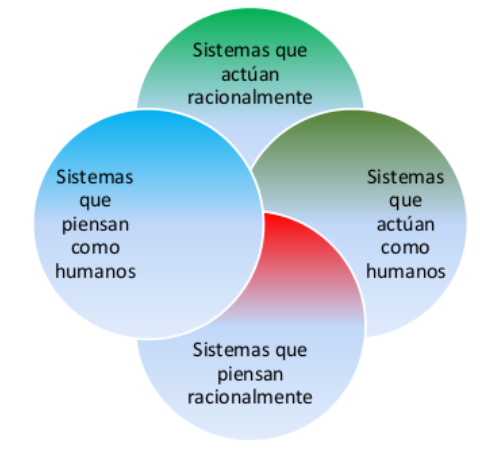
\includegraphics[width=9cm]{figs/Modelos de inteligencia.png}
    \end{center}
    \caption{Modelos de inteligencia}
    \label{fig:ModelosInteligencia}
\end{figure}

%La clasificación de los modelos de IA tiene un impacto significativo en las aplicaciones de la IA, ya que determina cómo se desarrollan y aplican los sistemas de inteligencia artificial en una amplia gama de campos, contribuyendo así a la mejora de la eficiencia y la innovación en muchas industrias donde se han ido desarrollando diferentes herramientas propias y aplicaciones, dando lugar a multitud de ramas que parten de la IA.\\

Una de las ramas más fascinantes y prometedoras de la inteligencia artificial es la visión artificial, que busca dotar a las máquinas de la capacidad de interpretar y comprender el mundo visual que les rodea. La siguiente sección se centra en la importancia de la IA y su intersección con la visión artificial, explorando cómo estas disciplinas se fusionan para mejorar la percepción y la comprensión de imágenes y vídeos.

\section{Visión Artificial}
\label{sec:VA} 

La visión artificial se define como la ciencia de programar un ordenador para procesar imágenes o vídeos e incluso entenderlos \cite{Culjak12}.\\

En \cite{Bradski08} se explica cómo es la transformación de datos desde un fotograma o vídeo cámara hasta lo que puede ser una decisión o una nueva representación \cite{Alvear17}. Para ello, la imagen percibida pasa por los procesos de obtención, caracterización e interpretación de información de imágenes; y estos procesos pueden ser subdivididos a su vez en \cite{Santillan15} según el Cuadro \ref{cuadro:procesos_VA}.\\

\begin{table} [H]
  \begin{center}
      \includegraphics[width=15cm, height=7cm]{figs/Procesos de la visión artificial.png}
  \end{center}
  \caption{Procesos de la visión artificial}
  \label{cuadro:procesos_VA}
\end{table}

\begin{enumerate}
 \item \textit{Captura:} %La captura o digitalización 
Es el proceso en el que se obtiene una imagen digital a partir de una imagen analógica a través de un dispositivo para que pueda ser manipulada por un ordenador. Esta imagen estará representada como una matriz de números (píxeles) \cite{Martinez22}.
 
 \item \textit{Pre-procesamiento:} En esta fase, se incorporan métodos destinados a restaurar las imágenes capturadas.%, dado que es factible que las imágenes experimenten deterioro.%, como la disminución de su claridad o la presencia de ruido. 
Esta etapa tiene como objetivo corregir estos problemas mediante procedimientos como la eliminación de ruido o la mejora del contraste y la nitidez.
 
 \item \textit{Segmentación:} %La segmentación 
Consiste en dividir una imagen en regiones o componentes más pequeños (grupo de píxeles) con el objetivo de identificar y aislar objetos o áreas de interés dentro de la imagen %El propósito principal es simplificar y organizar la información visual contenida en la imagen 
para que sea más fácil de analizar, comprender y procesar por ordenador.

 \item \textit{Descripción:} Es el proceso que obtiene características relevantes para poder diferenciar un tipo de objeto de otro, pudiendo ser externas, como la forma, el perímetro o el rectángulo mínimo que contiene la región; o internas, como el área o el centro de gravedad, entre otros \cite{Santillan15}. 
 
 \item \textit{Reconocimiento (clasificación):} %Esta fase se centra en identificar y asignar etiquetas o categorías a objetos o patrones previamente segmentados en una imagen o secuencia de imágenes. 
El proceso de reconocimiento implica el uso de algoritmos y técnicas de aprendizaje automático, como redes neuronales artificiales o métodos estadísticos, entre otros, para entrenar un modelo que pueda tomar las características extraídas y realizar predicciones sobre la clase o categoría a la que pertenecen los objetos detectados.
 
 \item \textit{Interpretación:} %Esta fase implica el análisis y comprensión del significado y el contexto de la información visual obtenida de las imágenes o la secuencia de imágenes capturadas. 
Esta etapa implica razonamiento, toma de decisiones y puede requerir el procesamiento de lenguaje natural para obtener una comprensión más profunda del contenido visual.
 
\end{enumerate}

Estas fases son las empleadas bajo el paradigma de lo que se conoce como Visión
Artificial Clásica, enfocada a la utilización de algoritmos específicos para procesar imágenes y reconocer en ellas características básicas \cite{Martinez22}.%, siendo generalmente secuenciales, a pesar de que los procesos que se utilicen en la resolución de un determinado problema dependen de su complejidad y no todas pueden ser siempre necesarias \cite{Santillan15}.\\
Sin embargo, para mejorar aún más la eficacia de los sistemas de visión artificial, se recurre al aprendizaje automático o \textit{machine learning} (ML). A continuación, profundizaremos en el papel del \textit{machine learning} en la visión artificial y su importancia en la creación de sistemas inteligentes de procesamiento de imágenes. 

\section{Machine Learning}
\label{sec:MachineLearning} 

El Machine Learning (Aprendizaje Automático) es una rama en evolución de la Inteligencia Artificial que se encarga de generar algoritmos que tienen la capacidad de aprender del entorno circundante y no tener que programarlos de manera explícita, teniendo en cuenta todos los escenarios posibles, a partir de la construcción de modelos analíticos \cite{Sandoval18}.\\ %Los aspectos clave y la semántica del machine learning se muestran en la Figura \ref{fig:ML semantics}.

% \begin{figure} [H]
%    \begin{center}
%      \includegraphics[width=14cm]{figs/ML semantics.png}
%    \end{center}
%    \caption{Aspectos clave y semántica del Aprendizaje automático}
%    \label{fig:ML semantics}
% \end{figure}

%En función del problema planteado y de los datos disponibles, se pueden distinguir tres tipos de ML:

%\begin{itemize}
% \item \textit{Aprendizaje supervisado:} Consiste en operar a partir de una expectativa conocida. %En este contexto, los conjuntos de datos de entrada se denominan conjuntos de datos etiquetados. 
%Los algoritmos clasificados en esta categoría se centran en establecer una relación entre los atributos de entrada y salida, y utilizan esta relación de forma especulativa para generar una salida para nuevos puntos de datos de entrada \cite{Gollapudi16}. 
 
% \item \textit{Aprendizaje no supervisado:} %El análisis o aprendizaje no supervisado 
%Se basa en el análisis de clasificación en el que no empezamos con un objetivo específico en mente, también denominado agrupación. En este caso, el objetivo es descifrar la estructura de los datos a partir de la construcción de un mapa entre los atributos de entrada y salida y, de hecho, los atributos de salida no están definidos %Estos algoritmos de aprendizaje operan sobre un conjunto de datos no etiquetados por esta razón
%\cite{Gollapudi16}.
 
% \item \textit{Aprendizaje por refuerzo:} En lugar de proporcionar pares de entrada y salida, se describe el estado actual del sistema, se especifica un objetivo proporcionando una lista de acciones permitidas y sus restricciones ambientales para sus resultados, y se deja que el modelo de ML experimente por sí mismo el proceso para alcanzar el objetivo utilizando el principio de ensayo y error para maximizar la recompensa del resultado \cite{Janiesch21}.
 
%\end{itemize}

%Del mismo modo, 
Dependiendo de la tarea de aprendizaje, existen varias clases de algoritmos de ML, cada uno de ellos con múltiples especificaciones y variantes, que pueden englobarse o bien en el Shallow Machine Learning (aprendizaje superficial), que se centra en algoritmos más simples para realizar tareas específicas, o en Deep Learning (aprendizaje profundo), que utiliza la construcción y entrenamiento de Redes Neuronales Artificiales (RNA), un tipo de modelo inspirado en la estructura y funcionamiento del cerebro humano, tal y como se puede apreciar en el diagrama de la Figura \ref{fig:AlgoritmosML} \cite{Janiesch21}. \\

 \begin{figure} [H]
    \begin{center}
      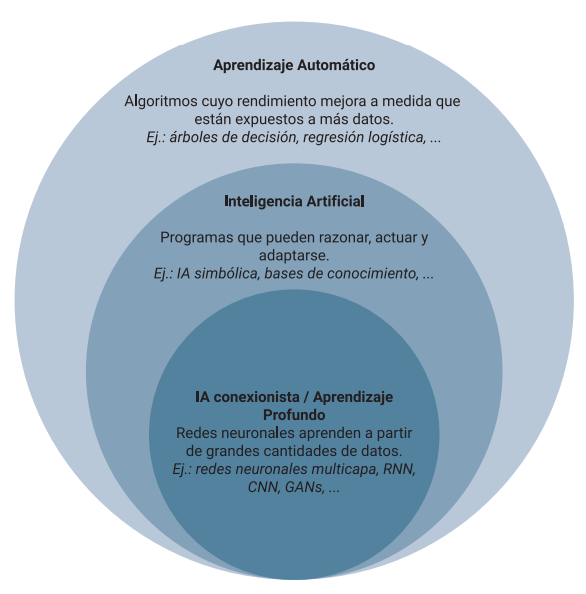
\includegraphics[width=9cm]{figs/Algoritmos de ML.png}
    \end{center}
    \caption{Diagrama de Venn de la relación entre distintas áreas de la IA}
    \label{fig:AlgoritmosML}
\end{figure}

El Machine Learning, abarca desde enfoques más superficiales hasta técnicas más avanzadas, tal y como se ha podido observar, sin embargo, es el Deep Learning lo que realmente potencia la capacidad de las máquinas para aprender y generalizar patrones complejos de manera excepcional. En la próxima sección, se hablará sobre el Deep Learning, centrándose en las RNA y en cómo estas posibilitan abordar tareas más complejas, como el reconocimiento de patrones en imágenes o el procesamiento de lenguaje natural.


\section{Deep Learning}
\label{sec:DeepLearning} 
El Deep Learning o aprendizaje profundo, constituye una rama de la IA, incluida dentro del Machine Learning, cuyos modelos computacionales se inspiran en el funcionamiento del cerebro humano y se diseñan con el propósito de adquirir conocimientos y llevar a cabo tareas específicas mediante el procesamiento de datos.\\ %La etiqueta \textit{profundo} hace referencia a la presencia de múltiples capas de neuronas artificiales en la red, lo que facilita la representación jerárquica de características y potencia la capacidad para aprender y poder diferenciar patrones complejos a partir de los datos.\\

Estas Redes Neuronales Artificiales (RNA) o Artificial Neural Networks (ANN) en inglés, están inspiradas en las redes neuronales biológicas del cerebro humano, tal y como muestra la Figura \ref{fig:Modelo neurona}, presentando características del mismo, ya que estas aprenden de la experiencia, generalizan de ejemplos previos a ejemplos nuevos, y abstraen las características principales de una serie de datos. En las RNA, la unidad análoga a la neurona biológica es el elemento procesador, PE (Process Element). Un PE tiene varias entradas y las combina, normalmente, con una suma básica. La suma de las entradas es modificada por una función de transferencia y el valor de la salida de esta función de transferencia se pasa directamente a la salida del elemento procesador. Existen dos capas con conexiones con el mundo exterior, una capa de entrada o \textit{buffer} de entrada, donde se presentan los datos a la red, y una capa o \textit{buffer} de salida que mantiene la respuesta de la red a una entrada, mientras que el resto de las capas reciben el nombre de capas ocultas \cite{Basogain08}.\\

\begin{figure} [H]
    \begin{center}
      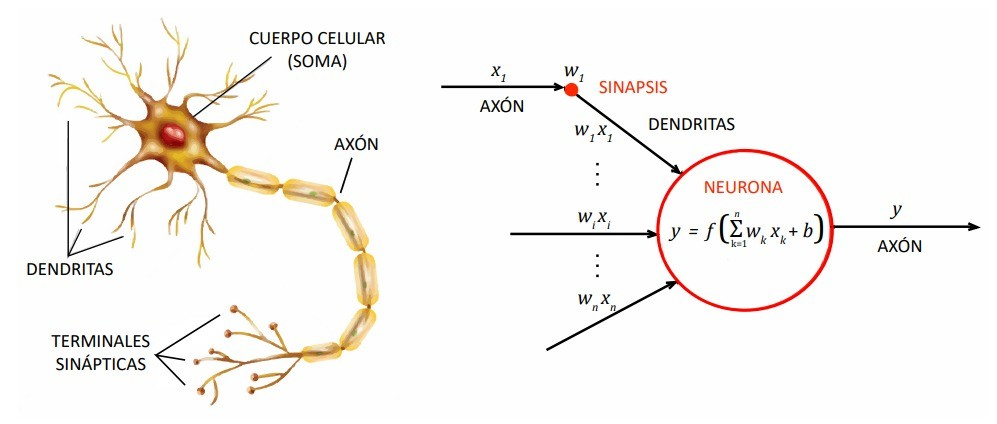
\includegraphics[width=15cm]{figs/Modelo neurona.jpeg}
    \end{center}
    \caption{Modelo biológico de una neurona genérica (izquierda) y el respectivo modelo matemático (derecha)}
    \label{fig:Modelo neurona}
\end{figure}

En consecuencia, se puede construir una red neuronal artificial mediante un conjunto de neuronas artificiales, es decir, mediante un conjunto de funciones, y conectando comúnmente la salida de cada una a las entradas de otras diferentes, como se representa en la Figura \ref{fig:Arquitectura red neuronal}. %De esta manera, las RNA no son más que redes de funciones, típicamente representadas mediante la composición de varias funciones, como se representa en la Figura \ref{fig:Arquitectura red neuronal}. Esto hace que los diferentes modelos de redes neuronales difieran principalmente en las funciones de activación utilizadas, el patrón de interconexión, e inclusive el tiempo de trasmisión de la información. 
Es importante señalar que la característica clave de la sinapsis, el escalar las señales de entrada por factores (pesos), es la manera en la que se cree que el cerebro aprende. Por lo tanto, distintos pesos dan como resultado diferentes respuestas a una entrada. De esta manera, se puede decir que el aprendizaje es el ajuste de los pesos en respuesta a un estímulo \cite{Dinamarca18}.\\

\begin{figure} [H]
    \begin{center}
      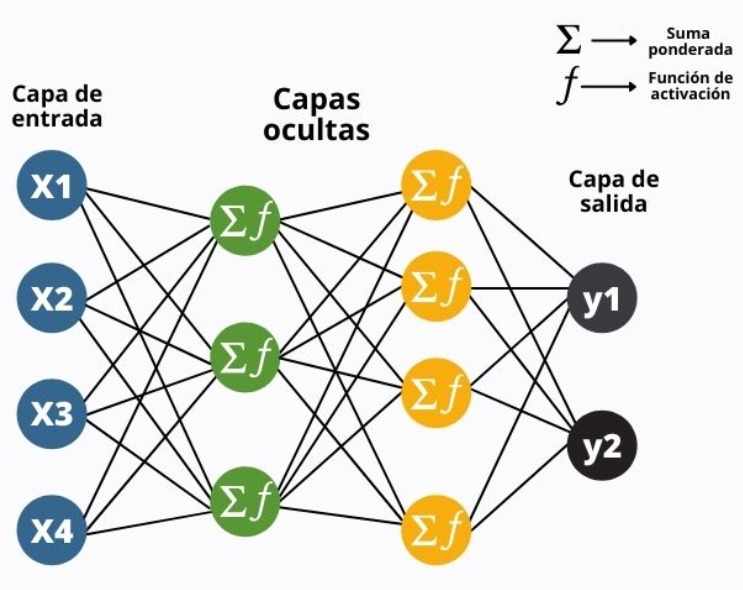
\includegraphics[width=9cm]{figs/capas rrnn.jpeg}
    \end{center}
    \caption{Arquitectura de una red neuronal}
    \label{fig:Arquitectura red neuronal}
\end{figure}

%La historia de las redes neuronales se remonta a la década de 1940, cuando el neurofisiólogo Warren McCulloch y el matemático Walter Pitts modelaron una red neuronal simple utilizando circuitos eléctricos. Su modelo estaba basado en la idea de lógica de umbral, que más tarde sería fundamental para el desarrollo de las redes neuronales artificiales. En 1958, el neurobiólogo Frank Rosenblatt dio un paso significativo al comenzar a trabajar en el perceptrón, un modelo computacional que representaba la unidad básica de una red neuronal y realizaba una suma ponderada de varias entradas, al tratarse de una unidad de procesamiento, llevando a cabo una combinación lineal de esas entradas, y aplicando posteriormente una función de activación para producir una salida. Este trabajo marcó el inicio de la investigación en redes neuronales artificiales. Saltando a la década de 2010, dos factores contribuirían a la revolución de aplicaciones de redes neuronales y algoritmos de aprendizaje profundo. En primer lugar, los avances en hardware especializado aceleraron drásticamente el entrenamiento y el rendimiento de las redes neuronales, reduciendo su consumo de energía, mientras que, en segundo lugar, el aumento de datos abiertos disponibles en línea y servicios de bajo costo para etiquetar datos impulsaron el desarrollo de la inteligencia artificial \cite{Abeliuk21}.\\

\vspace{10mm}

En este capítulo se ha introducido el nacimiento y la historia de los robots y la robótica tal y como los conocemos hoy en día, dentro de cuya rama encontramos uno de los tres grandes grupos en los cuales puede dividirse esta, la Robótica de Servicio, y para la que la Inteligencia Artificial, y más concretamente el campo de la Visión Artificial junto con el del Deep Learning, siendo este subcategoría del Machine Learning, juegan un papel fundamental en el desarrollo de nuevas aplicaciones.\\

En este proyecto se presenta un sistema que, mediante Visión Artificial y Machine Learning, es capaz de reconocer la maduración de frutos, más concretamente de fresas, con el objetivo de poder ayudar así a mejorar su proceso de recolección en un huerto vertical, gracias al algoritmo desarrollado para esto y su integración con un brazo robótico de la marca Universal Robots, que se encargará de llevar a cabo este proceso.\\
\\
\\
\\
En los siguientes capítulos de este trabajo se detallarán los objetivos del mismo, delineando claramente las metas; se expondrá la plataforma de desarrollo, detallando las herramientas seleccionadas para la elaboración del proyecto; se presentará el diseño y la arquitectura del proyecto; y, finalmente, llegaremos a las conclusiones, donde tendrá lugar una breve recopilación de información sobre los resultados obtenidos y las posibles direcciones futuras. 


\setlength{\parskip}{0.7em} % Espaciado vertical entre p�rrafos
\chapter{Estado del arte}
\label{cap:capitulo2}
	
En el presente capítulo, se van a describir algunos de los prototipos y soluciones más destacables aplicadas a la detección y recolección de fresas usando inteligencia artificial y técnicas robóticas.\\

\section{Descripción del problema}
\label{sec:descripcion}

Cuenta aquí el objetivo u objetivos generales y, a continuación, concrétalos mediante objetivos específicos.

\section{Requisitos}
\label{sec:requisitos}

Describe los requisitos que ha de cumplir tu trabajo.

\section{Metodología}
\label{sec:metodologia}

Qué paradigma de desarrollo software has seguido para alcanzar tus objetivos.

\section{Plan de trabajo}
\label{sec:plantrabajo}

Qué agenda has seguido. Si has ido manteniendo reuniones semanales, cumplimentando objetivos parciales, si has ido afinando poco a poco un producto final completo, etc.


\setlength{\parskip}{0.7em} % Espaciado vertical entre p�rrafos
\chapter{Objetivos}
\label{cap:capitulo3}
\setcounter{footnote}{12}
 
Una vez presentado el contexto general en el cual se enmarca el presente trabajo de fin de grado, en este capítulo se describen los objetivos y requisitos de este, así como la metodología y el plan de trabajo llevados a cabo.

\section{Descripción del problema}
\label{sec:descripcion}

La necesidad de implementar soluciones tecnológicas que automaticen y optimicen las tareas de recolección incrementando la eficiencia en la recolección, mejorando la calidad del producto y disminuyendo los costes asociados, surge debido a la situación actual de la agricultura en la que, uno de los mayores desafíos que enfrenta es la recolección de frutas y hortalizas, problema que deriva de la escasa mano de obra disponible y el proceso manual que esto conlleva.%, y de la posibilidad de que existan errores humanos en la identificación de los frutos para su recolección, pudiendo influenciar esto en la calidad del producto, especialmente en la recolección de frutos que requieren un manejo cuidadoso, como las fresas.\\

La solución propuesta en este trabajo busca ayudar a mejorar esta situación, proporcionando un robot de bajo coste y accesible a cualquier persona, que sirva para poder mejorar el proceso de reconocimiento por visión de la maduración de frutos, más concretamente fresas, para su posterior recolección. Por lo tanto, este proyecto pretende, como objetivo principal, utilizar un robot colaborativo que, gracias a su interfaz intuitiva sea accesible a cualquier persona y, junto con el sistema de detección elaborado con materiales de bajo coste, sea capaz de reconocer las fresas maduras de un sistema de cultivo agrícola vertical, para su posterior recolección por el brazo robótico, gracias a la comunicación establecida entre el sistema de visión y el robot.

Con el fin de alcanzar este objetivo principal, se han establecido los siguientes
subobjetivos:

\begin{enumerate}
  \item Investigar las soluciones actuales que cumplen con las características y objetivos establecidos.
  \item Seleccionar la técnica de inteligencia artificial de reconocimiento de frutas y seleccionar los componentes hardware necesarios para desarrollar el sistema de visión de bajo coste más eficiente.
  \item Optimizar la técnica escogida y adaptarla de tal manera que sea capaz de funcionar en nuestra plataforma. Al ser una técnica basada en Machine Learning, se deberá crear un dataset con imágenes de fresas y, por lo tanto, hacer un correcto tratamiento de los datos para conseguir un resultado preciso en el posterior entrenamiento.
  \item Realizar el entrenamiento con varios algoritmos de Machine Learning de
clasificación. Estudiar el rendimiento y precisión de cada uno de ellos a través de pruebas con el sistema de visión y fresas reales.
  \item Seleccionar el protocolo de comunicación entre el sistema de visión y el robot y llevar a cabo pruebas; tanto simuladas, a través del simulador que facilita el fabricante del robot, como reales, para establecer esta comunicación.
  \item Dar soporte software al robot mediante un %Programación tanto del robot como del archivo en Python que posee el código del 
sistema de reconocimiento de fresas, que guarde las posiciones y la distancia de estas a la posición de la cámara, para su posterior envío al brazo robótico.
  \item Realizar pruebas de la aplicación final, tanto en entornos simulados como reales.
\end{enumerate} 
 
\section{Plan de trabajo}
\label{sec:plantrabajo}
El desarrollo y seguimiento que el proyecto ha seguido es una planificación en base a reuniones semanales con el tutor, en las cuales se revisaron los avances, se fijaron nuevos objetivos y se discutieron y propusieron posibles mejoras, mientras que el trabajo se organizó en varias fases clave: 
\begin{enumerate}
  \item \textit{Investigación inicial:} En esta fase, se investigó el estado del arte relacionado con sistemas de visión artificial y técnicas de reconocimiento de objetos, especialmente aplicadas a la maduración de frutas y hortalizas, y utilizando para ello artículos científicos, capítulos de libros y proyectos previos. 
  \item \textit{Diseño y desarrollo del sistema de visión artificial:} Esta fase se centró en el diseño y la implementación del sistema de visión artificial, abarcando tanto el desarrollo del software como la integración del hardware, e incluyendo la calibración y obtención de los parámetros intrínsecos a la cámara y las diversas pruebas realizadas con distintos sistemas y códigos, hasta seleccionar el \textit{software} funcional con el que se llevó a cabo el proyecto finalmente.
  \item \textit{Pruebas en entorno simulado:} Durante esta fase se realizaron múltiples pruebas y ajustes para optimizar el funcionamiento del sistema y comprobar su funcionamiento en diferentes escenarios, simulando de manera separada la programación del robot, para el que se utilizó un simulador en una máquina virtual, y la detección y funcionamiento del sistema de visión, cuyos algoritmos se afinaron para mejorar la precisión en la detección y se ajustaron los parámetros relacionados con la cámara en los códigos para poder obtener las coordenadas y distancia real de las detecciones respecto a la cámara y poder transmitírselas al brazo robótico. Finalmente, también se llevaron a cabo pruebas de comunicación entre el sistema de visión y el robot, poniendo a prueba su programación, para que este alcanzase el punto de la detección.
  \item \textit{Pruebas en entorno real:} Una vez desarrollado el prototipo inicial, el sistema completo fue sometido a pruebas en un entorno real de lo que sería la aplicación final. 
  \item \textit{Escritura de la memoria:} Con el sistema ya afinado y probado, se procedió a la redacción de la memoria del proyecto. En esta etapa, se documentó detalladamente todo el proceso seguido, desde la investigación inicial hasta los resultados finales obtenidos durante las pruebas reales. 
\end{enumerate}


Todo el contenido del proyecto se puede encontrar en un repositorio público de GitHub\footnote{\url{https://github.com/RoboticsURJC/tfg-dcampoamor}}, en cuya wiki\footnote{\url{https://github.com/RoboticsURJC/tfg-dcampoamor/wiki}} se puede ver el desarrollo del trabajo en semanas a lo largo de los meses, durante el trascurso del proyecto. Las requisitos necesarios para la consecución de los objetivos planteados, las competencias desarrolladas y la metodología empleada pueden encontrarse descritos en el Anexo \ref{cap:capitulo7}.
%Después de haber revisado los objetivos, requisitos, competencias, metodología y el plan de trabajo implementado para la realización de este proyecto, en el siguiente capítulo se abordarán las plataformas de desarrollo empleadas.



\setlength{\parskip}{0.7em} % Espaciado vertical entre p�rrafos
\chapter{Plataforma de desarrollo}
\label{cap:capitulo4}
 
Con los objetivos del proyecto definidos, en este capítulo se abordarán las distintas plataformas de desarrollo, tanto \textit{hardware} como \textit{software}, que han facilitado el logro de esos objetivos.

\section{Hardware}
\label{sec:hardware}

Este apartado recoge la descripción de los componentes \textit{hardware} utilizados en este proyecto, para los cuales se ha buscado priorizar la reducción de costes en cada elección y utilizar aquellos elementos a los que se tenía acceso al desarrollar el proyecto.

\subsection{Cámara Logitech C270 HD}
\label{subsec:logiC270HD}

Esta cámara web (Figura \ref{fig:logiC270HD}) de dimensiones 72,91 x 31,91 x 66,64 mm, corrige la iluminación de manera automática, produciendo colores reales y naturales y ajustándose a las condiciones de iluminación del entorno, lo que facilita la detección de fresas. Ofrece una resolución HD 720p, proporcionando imágenes claras y nítidas a una velocidad de 30 fotogramas por segundo (fps), con una lente que cuenta con enfoque fijo y un campo visual diagonal (dFoV) de 55 grados. Su coste aproximado es de entre 30-40€.

\begin{figure} [H]
    \begin{center}
      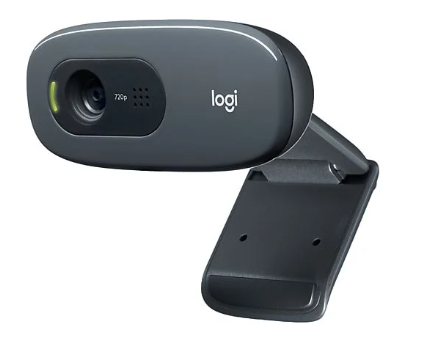
\includegraphics[width=5cm]{figs/logi C270.png}
    \end{center}
    \caption{Cámara Logitech C270 HD$^{\ref{note:enlace16}}$}
    \label{fig:logiC270HD}
\end{figure}

\setcounter{footnote}{16}
\footnotetext[\value{footnote}]{\url{https://www.logitech.com/es-es/products/webcams/c270-hd-webcam.960-001063.html?srsltid=AfmBOor4HptUTcGrxE-4SZxKR-ARw-ykNeagHSEzXUvTlXkx8qLfY4lG}\label{note:enlace16}}

\subsection{Soporte de brazo articulado}
\label{subsec:soporte_camara}

Para poder ubicar la cámara en una posición fija desde la cual visualizar las fresas, se utilizó un soporte de brazo articulado (Figura \ref{fig:soporte_camara}), cuya parte fija en la parte inferior se ancla a la mesa. Este soporte articulado tiene un ajuste de 360 grados, con su extremo más largo de 75 cm, mientras que la carga máxima que permite es de 560 gramos cuando se coloca de manera horizontal, siendo el precio de este soprte 22,98€.

\begin{figure} [H]
    \begin{center}
      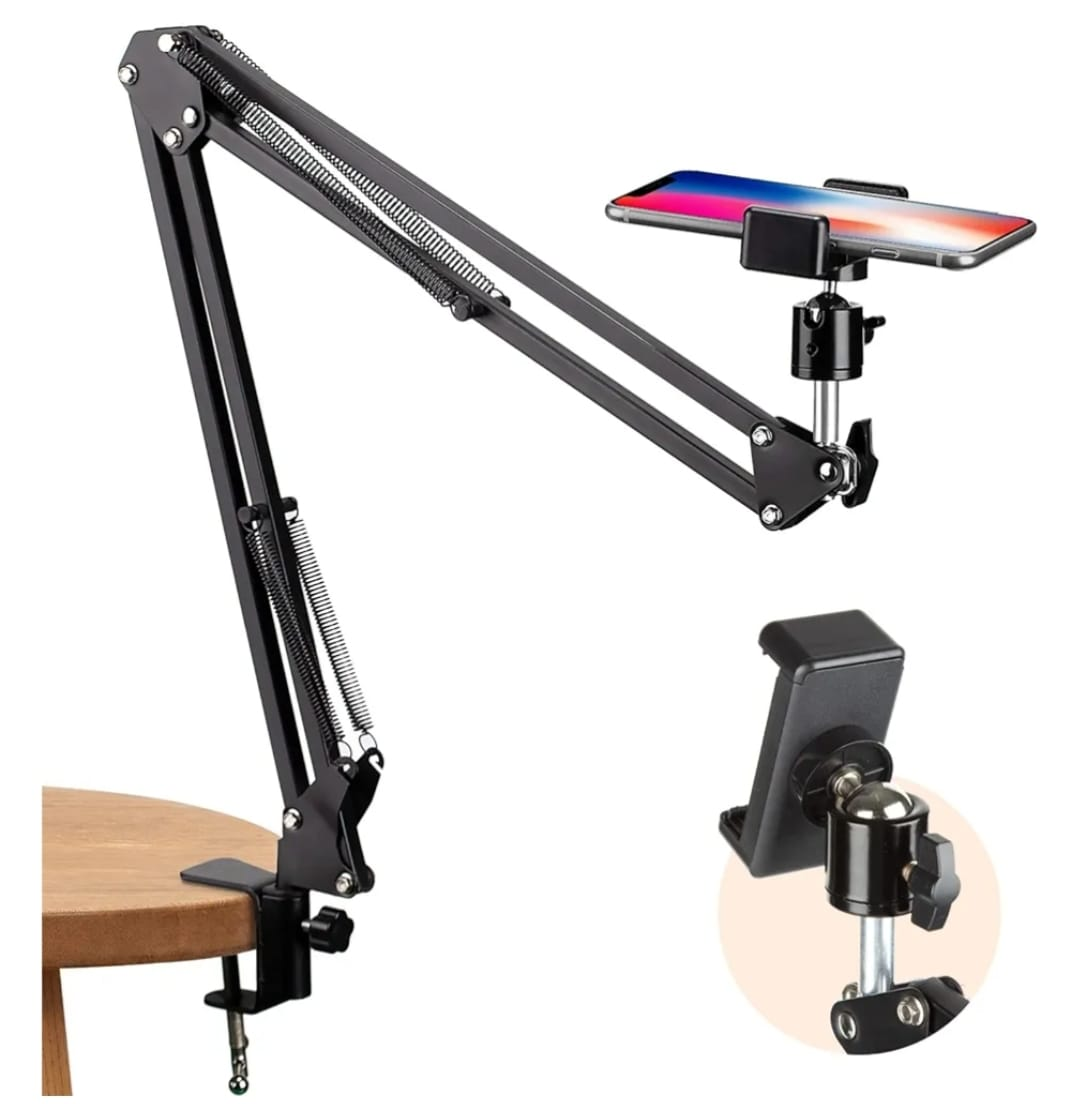
\includegraphics[width=5cm]{figs/Soporte de brazo articulado.jpeg}
    \end{center}
    \caption{Soporte de brazo articulado$^{\ref{note:enlace17}}$}
    \label{fig:soporte_camara}
\end{figure}
 
\setcounter{footnote}{17} 
\footnotetext[\value{footnote}]{\url{https://www.amazon.es/dp/B08JCG4V5S?ref=ppx_pop_mob_ap_share&th=1}\label{note:enlace17}}

\subsection{Ordenador principal}
\label{subsec:ordenador}

El equipo que se ha configurado como entorno de trabajo para este proyecto es el que aparece en la Figura \ref{fig:PC_Lenovo}, sirviendo como base para el desarrollo de la programación y las pruebas de la visión artificial, y utilizándose igualmente como servidor para poder llevar a cabo la comunicación con el brazo robótico mediante el protocolo XML-RPC basado en HTTP, y posteriormente el envío de posiciones detectadas en tiempo real a este. 

\begin{figure} [H]
    \begin{center}
      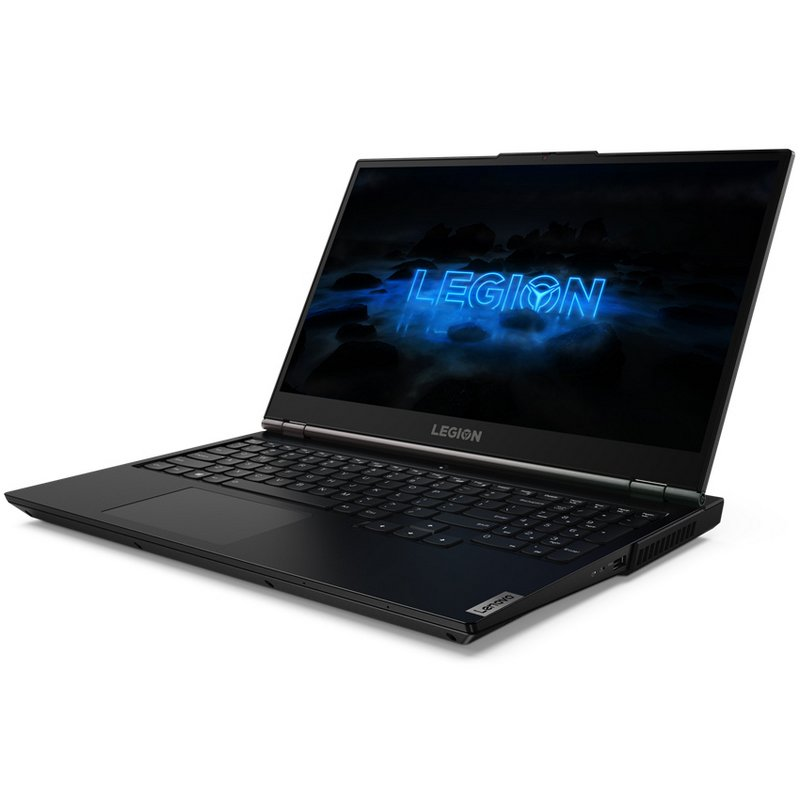
\includegraphics[width=7cm]{figs/Lenovo Legion 5 15imh05.jpg}
    \end{center}
    \caption{Lenovo Legion 5 15IMH05$^{\ref{note:enlace18}}$}
    \label{fig:PC_Lenovo}
\end{figure}

\setcounter{footnote}{18}
\footnotetext[\value{footnote}]{%
    https://www.pccomponentes.com/lenovo-legion-5-15imh05-intel-core-i7-10750h-16gb-1tb-ssd-gtx-1650-156?srsltid=AfmBOopJpvGSHUyQU696jgG7-6orSKMOEWZe2ZvvYtA0NGtJ9Ms2xJFp%
    \label{note:enlace18}%
}
    
A continuación, en el Cuadro \ref{cuadro:carac_ordena}, se recogen las características técnicas del ordenador utilizado:

\begin{table}[H]
	\begin{center}
		\begin{tabular}{|c|c|}
			\hline
			\textbf{Características} & \textbf{Descripción} \\
			\hline
			\multirow{2}{*}{Pantalla} & \multirow{2}{*}{\shortstack{15,6 pulgadas \\ Full HD (1920x1080)}} \\
			& \\
			\hline
			Procesador (CPU) & Intel Core i7-10750H CPU @ 2.60GHz \\
			\hline
			Memoria RAM & 16 GB \\
			\hline
			Almacenamiento & 1 TB \\
			\hline
			Tarjeta gráfica (GPU) & NVIDIA GeForce GTX 1650 Ti Mobile \\
			\hline
			Sistema Operativo & Windows 10 y Ubuntu 22.04.4 LTS \\
			\hline
			Cámara de portátil & HD 720p con tapa de privacidad \\
			\hline
			\multirow{5}{*}{Puertos} & \multirow{5}{*}{\shortstack{4 x USB 3.2 Gen 1 Tipo-A \\ 1 x USB 3.2 Gen 1 Tipo-C \\ 1 x Ethernet (RJ-45) \\ 1 x HDMI 2.0 \\ 1 x combo auriculares/micrófono (3.5 mm)}} \\
			& \\
			& \\
			& \\
			& \\
			\hline
			Conectividad & WiFi 6 802.11ax (2x2), Bluetooth 5.0, Ethernet 100/1000M \\
			\hline
			Batería & 80 Wh \\
			\hline
			Peso & 2,3 kg \\
			\hline
			Dimensiones & 363,06 x 259,61 x 23,57--26,1 mm \\
			\hline
		\end{tabular}
		\caption{Especificaciones técnicas del ordenador usado}
		\label{cuadro:carac_ordena}
	\end{center}
\end{table}

\subsection{Robot de \textit{Universal Robots} de la gama \textit{e-series}}
\label{subsec:URe-series}

Los robots de Universal Robots, también conocidos como robots colaborativos o cobots, están diseñados para trabajar junto a los humanos de manera segura, eficiente y flexible tanto en aplicaciones industriales como no industriales, destacando por su facilidad de uso, versatilidad y capacidad para automatizar tareas repetitivas o peligrosas \cite{UR_e-series_brochure18}. 

Fabricados en aluminio junto con otros materiales de bajo peso, %permitiendo reducir la inercia del propio robot y facilitar su manipulación, 
cada brazo robótico tiene seis ejes, otorgando al robot seis grados de libertad (Degree Of Freedom o DOF), que permiten movimientos precisos y fluidos, y en cuyas articulaciones están equipadas, a su vez, encoders absolutos, reductoras armónicas, que reducen la velocidad de rotación de los engranajes en las juntas, y aumentan el par del eje, ofreciendo una alta precisión y eficiencia; y, en aquellos brazos robóticos pertenecientes a la gama e-series, sensores de fuerza y torque, encontrándose integrados en el efector o tool flange del propio brazo robótico\footnote{\url{https://www.universal-robots.com/mx/acerca-de-universal-robots/noticias/meet-the
-next-generation-of-collaborative-ur-robots-at-robobusiness}}. 

%Por otro lado, en la controladora de los brazos robóticos de la gama e-series, pueden diferenciarse varios módulos \cite{Service_Manual_UR_e-series_2024}: 

%\begin{itemize}
%    \item Unidad de procesamiento principal (CPU): que se encarga de realizar los cálculos cinemáticos y dinámicos del robot, la ejecución de programas y control del brazo robótico mediante su software Polyscope, junto con la comunicación con los periféricos y la consola de mando o teach pendant.
%    \item Fuente de alimentación: que suministra energía a todos los componentes del sistema, incluyendo a las articulaciones del brazo robótico y el teach pendant, y que incluye protección contra sobrecargas y cortocircuitos para garantizar una alimentación estable y segura.
%    \item Módulo de seguridad o la placa de seguridad (Safety Control Board o SCB): que implementa funciones de seguridad colaborativa, como límites de velocidad, fuerza y espacio de trabajo, y que supervisa las entradas de seguridad y gestiona las paradas de emergencia.
%    \item Interfaces de comunicación: compuesta del puerto ethernet, que soporta los protocolos de comunicación TCP/IP, ModbusTCP, ProfiNet y EthernetIP,  los dos puertos USB (uno de ellos USB 2.0 y otro USB 3.0), las dieciseis entradas y salidas digitales, y las dos entradas y salidas analógicas.
%    \item Sistema de refrigeración: compuesto por ventiladores internos, que están controlados por sensores térmicos que ajustan su velocidad en función de la temperatura interna de los componentes, llegando a activar alarmas si se detectasen temperaturas anormales, rejillas de ventilación en el lateral de la carcasa o envolvente de acero que recubre y protege los componentes internos de la controladora, que a su vez están protegidas por filtros para evitar la entrada de polvo o partículas grandes. 
%    \item Módulo de almacenamiento interno: espacio dedicado para guardar y almacenar el sistema operativo basado en Linux y el software de la interfaz gráfica y entorno de programación del robot llamado Polyscope, programas, configuraciones, y datos operativos del robot como registros de eventos de datos de diagnóstico. Para esta gama de robots se utiliza una tarjeta SD de almacenamiento interno.
%\end{itemize}

Para el desarrollo de este proyecto se han utilizado diferentes modelos de robots de la gama e-series, todos ellos representados en la Figura \ref{fig:Gama_e-series}, desde el UR3e \cite{User_Manual_UR3e_2025} hasta el UR10e \cite{User_Manual_UR10e_2025}, pasando por el UR5e  \cite{User_Manual_UR5e_2025} .
A pesar de que tanto la gama CB-series como la gama e-series permiten la comunicación mediante el protocolo XML-RPC, la interfaz más intuitiva y simplificada que facilita la programación y reduce la sobrecarga de información, poseer sensor de fuerza integrado, permitiendo un control más preciso y sensible haciendo que mejore la interacción con el entorno, así como una mayor precisión en la repetición de movimientos, entre otros factores, constituyeron que se eligiera la gama e-series para este trabajo \cite{Service_Manual_UR_e-series_2024}.

\begin{figure} [H]
    \begin{center}
      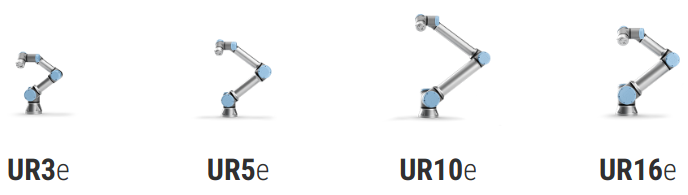
\includegraphics[width=16cm]{figs/Gama e-series.png}
    \end{center}
    \caption{Gama e-series de Universal Robots$^{\ref{note:enlace20}}$}
    \label{fig:Gama_e-series}
\end{figure}

\setcounter{footnote}{20} 
\footnotetext[\value{footnote}]{\url{https://www.universal-robots.com/es/productos/}\label{note:enlace20}}


\subsection{Comunicaciones}
\label{subsec:comunicacion}

En este proyecto, la comunicación entre el robot y el ordenador que ejecuta el servidor XML-RPC se establece vía Ethernet, permitiendo una conexión rápida y confiable. La infraestructura de red juega un papel fundamental en esta comunicación, ya que el robot y el servidor deben estar correctamente configurados dentro de la misma red, por lo que se emplea un switch Ethernet, en este caso el TP-Link LS105G %(Figura \ref{fig:TPLink_LS105G})
, para gestionar las conexiones entre los diferentes dispositivos y asegurar una comunicación fluida y sin interferencias.

Este switch de escritorio, cuyo precio es de 14,90€,  posee cinco puertos Ethernet RJ45 a 10/100/1000 Megabits por segundo (Mbps), permitiendo la transferencia instanténea de archivos y paquetes, con gran ancho de banda y sin interferencias, y no necesita configuración manual previa, ya que se trata de un dispositivo \emph{plug and play}, por lo que simplemente se tiene que conectar y empieza a funcionar. 

%\begin{figure} [H]
%    \begin{center}
%      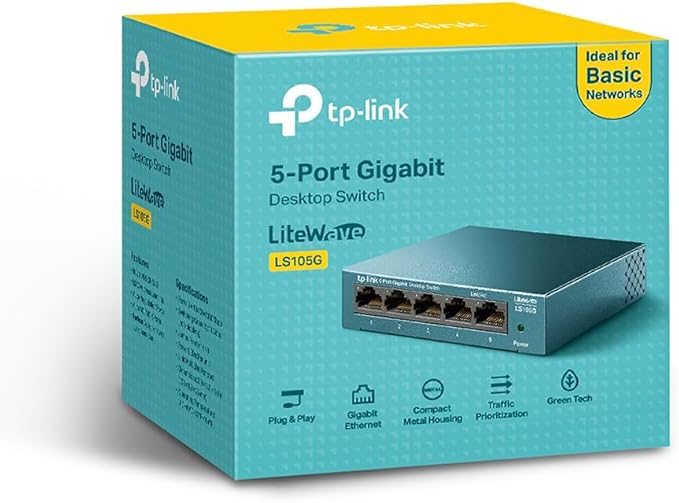
\includegraphics[width=6cm]{figs/TPLink LS105G.jpg}
%    \end{center}
%    \caption{Switch TP-Link LS105G$^{\ref{note:enlace21}}$}
%    \label{fig:TPLink_LS105G}
%\end{figure}

\setcounter{footnote}{21} 
\footnotetext[\value{footnote}]{\url{https://www.tp-link.com/es/business-networking/litewave-switch/ls105g/}\label{note:enlace21}}

\section{Software}
\label{sec:software}

Este apartado estará dedicado a detallar las plataformas de software, librerías y entornos de trabajo que han sido fundamentales para alcanzar los objetivos definidos en el Capítulo 3, desde el sistema operativo utilizado hasta las tecnologías específicas para el procesamiento de imágenes y aprendizaje profundo.

\subsection{Ubuntu}
\label{sec:ubuntu}
Ubuntu\footnote{\url{https://ubuntu.com/}} es un sistema operativo de código abierto basado en Linux y desarrollado por la empresa británica Canonical Ltd. 
Este sistema operativo está diseñado para ser utilizado en una gran variedad de dispositivos, y es reconocido por su facilidad de uso, estabilidad y seguridad, contando con una amplia comunidad de desarrolladores y usuarios que contribuyen activamente a su desarrollo y soporte. La versión utilizada para la realización de este proyecto, de entre todas las versiones disponibles, es Ubuntu 22.04 Long Term Support (LTS) (Jammy Jellyfish), ya que era la última versión disponible de Ubuntu en el momento en el que se empezó a elaborar el proyecto. 

\subsection{Polyscope}
\label{sec:Polyscope}

Polyscope\footnote{\url{https://www.universal-robots.com/es/productos/polyscope/}} es la interfaz de usuario gráfica desarrollada por Universal Robots para poder programar y utilizar sus robots colaborativos. Está diseñada para ser intuitiva y accesible, ya que permite a los usuarios crear programas de robot sin necesidad de conocimientos avanzados en programación. 

Construido sobre una plataforma basada en Linux, PolyScope está basado en una arquitectura de software que combina una interfaz gráfica amigable con un lenguaje de programación propio llamado URScript, permitiendo tanto a usuarios sin experiencia en programación como a programadores avanzados interactuar eficazmente con los robots UR, ya que la interfaz gráfica facilita la creación de programas mediante bloques visuales, mientras que URScript ofrece una mayor flexibilidad para desarrollos más complejos.

A lo largo de los años, Universal Robots ha lanzado varias versiones de PolyScope, cada una con mejoras y nuevas funcionalidades, siendo la primera versión PolyScope 3, lanzada en 2012, ya que fue diseñada para la serie CB3 de robots UR. PolyScope 5\footnote{\url{https://www.universal-robots.com/products/polyscope-5/}} (Figura \ref{fig:Polyscope5}) se introdujo en junio de 2018, coincidiendo con el lanzamiento de la gama de robots e-series de Universal Robots. Por último, PolyScope X\footnote{\url{https://www.universal-robots.com/products/polyscope-x/}} es la última evolución del software de Universal Robots, siendo su lanzamiento oficial en noviembre de 2024\footnote{\url{https://www.universal-robots.com/2024q3/polyscope-x-festival/}}, y estando basado en tecnologías como ROS2 y contenedores Docker, centraliza las funciones más importantes y simplifica la programación mediante el uso de plantillas predefinidas. %, incluyendo mejoras respecto a Polyscope 3 en la interfaz de usuario (Figura \ref{fig:Polyscope5}), haciéndola más intuitiva y moderna y facilitando la programación y configuración del robot, incluyendo nuevas funcionalidades de seguridad como la capacidad de restringir la entrada de una esfera virtual en una zona o plano de seguridad y establecer límites de velocidad y distancia de frenado mejorando la seguridad en el entorno de trabajo; incrementando la frecuencia de control a 500 hercios (Hz) permitiendo de esta manera movimientos más precisos e incorporando soporte para nuevas características de hardware como la interfaz de comunicación de herramientas (Tool Communication Interface) en la que el conector de herramientas puede utilizarse para la comunicación serie RS485 con una velocidad de datos de hasta 5 megabits\footnote{\url{https://forum.universal-robots.com/t/release-of-e-series-polyscope-5-0-polyscope-3-6-sdk-1-3-and-a-brand-new-developer-community}}.

\begin{figure} [H]
    \begin{center}
      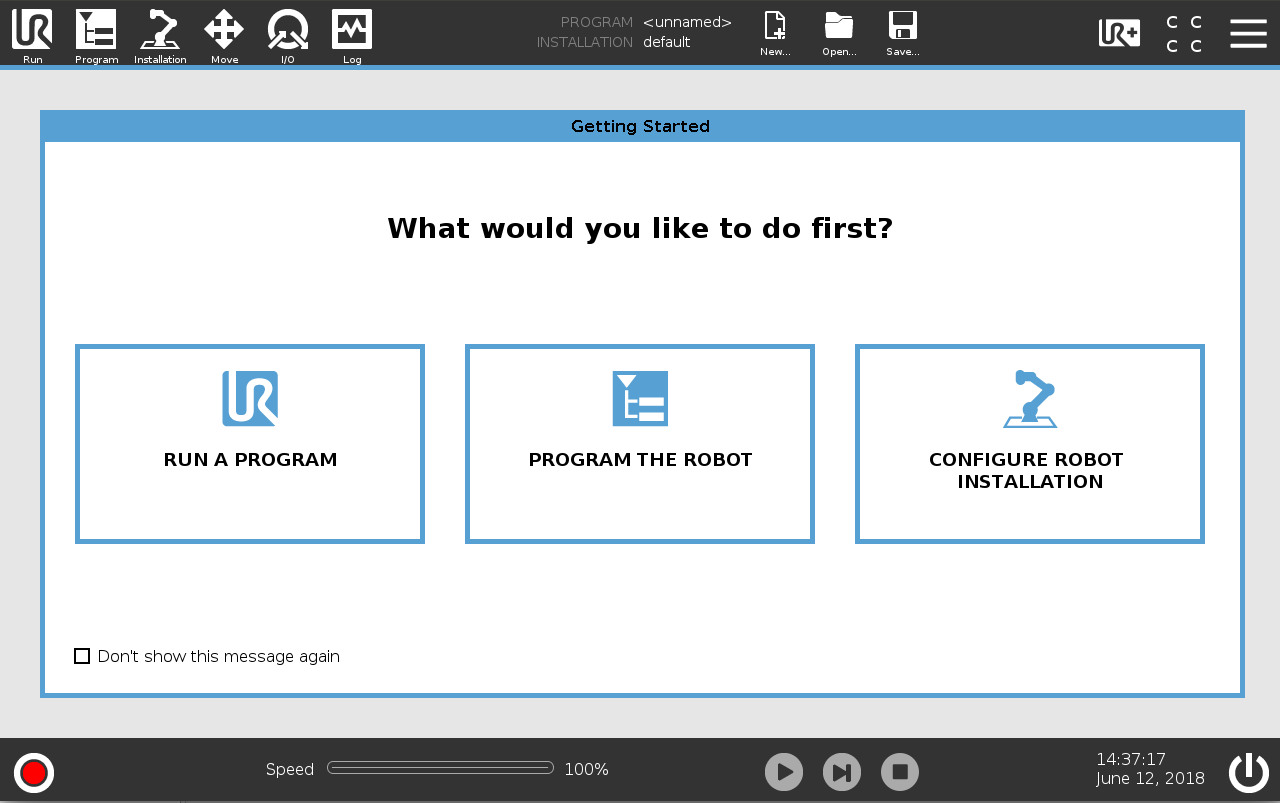
\includegraphics[width=15cm]{figs/InterfazPolyscope5.png}
    \end{center}
    \caption{Pantalla principal de la interfaz de Polyscope 5}
    \label{fig:Polyscope5}
\end{figure}

%Por último, PolyScope X\footnote{\url{https://www.universal-robots.com/products/polyscope-x/}} es la última evolución del software de Universal Robots, diseñado para simplificar y potenciar los procesos de automatización, %Aunque se presentó un prototipo en la feria International Manufacturing Technology Show (IMTS) en 2022 y se mostró en Automatica en Múnich en junio de 2023, siendo su lanzamiento oficial en noviembre de 2024\footnote{\url{https://www.universal-robots.com/2024q3/polyscope-x-festival/}}. Basado en tecnologías como ROS2 y contenedores Docker, ofrece una plataforma más flexible y escalable para el desarrollo y la integración de aplicaciones,%modificando de nuevo la interfaz de usuario (Figura \ref{fig:PolyscopeX}) respecto a Polyscope 5, centralizando las funciones más importantes y simplificando la programación mediante el uso de plantillas predefinidas. %para agilizar y facilitar la creación de módulos reutilizables y simplificando la programación a los operarios, reduciendo de esta manera la complejidad en el desarrollo de aplicaciones.

%\begin{figure} [H]
%    \begin{center}
%      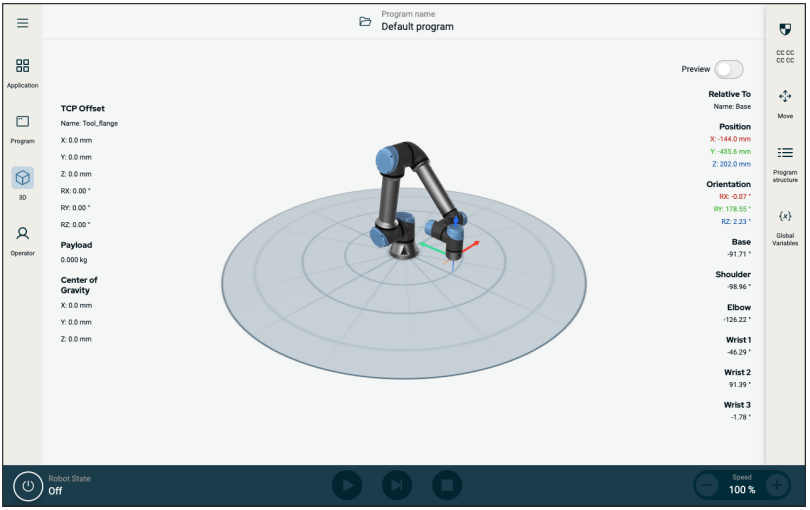
\includegraphics[width=13cm]{figs/InterfazPolyscopeX.png}
%    \end{center}
%    \caption{Pantalla principal de la interfaz de Polyscope X}
%    \label{fig:PolyscopeX}
%\end{figure}

A pesar de que Polyscope X es compatible con los robots de la gama e-series, se deben cumplir una serie de requisitos en cuanto al hardware de la controladora para poder actualizar desde Polyscope 5, por lo que para el desarrollo de este proyecto se ha terminado utilizado la versión 5.16 de Polyscope 5, puesto que no se cumplían todos los requisitos para que se diera esta actualización en los robots utilizados.

\subsection{Python}
\label{sec:python}
Python\footnote{\url{https://www.python.org/}} es un lenguaje de programación de alto nivel, orientado a objetos y de semántica dinámica. La sintaxis de Python, sencilla y fácil de aprender, favorece la legibilidad y, por tanto, reduce el coste de mantenimiento de los programas, admitiendo módulos y paquetes, lo que fomenta la modularidad del programa y la reutilización de código \footnote{\url{https://www.python.org/doc/essays/blurb/}} para el desarrollo de aplicaciones en diferentes áreas, como sucede en este caso con la inteligencia y visión artificial y el aprendizaje automático. 
\pagebreak

\subsection{PyTorch}
\label{sec:PyTorch}

De los desarrolladores de Facebook AI Research junto a otros laboratorios, PyTorch\footnote{\url{https://pytorch.org/}} es un marco de aprendizaje profundo de código abierto conocido por su compatibilidad con Python, siendo un marco de trabajo completo para crear modelos de aprendizaje profundo. Se distingue por su excelente compatibilidad con GPU y su uso de la autodiferenciación en modo inverso, que permite modificar los gráficos de cálculo sobre la marcha, lo que lo convierte en una opción popular para la experimentación rápida y la creación de prototipos.

\subsection{NumPy}
\label{sec:NumPy}

NumPy (Numerical Python)\footnote{\url{https://numpy.org/}} es una biblioteca de Python fundamental para el cálculo numérico, que proporciona un objeto de matriz multidimensional, varios objetos derivados (como matrices y matrices enmascaradas) y un surtido de rutinas para realizar operaciones rápidas con matrices \footnote{\url{https://numpy.org/doc/stable/user/whatisnumpy.html/}}. 

En este proyecto, la biblioteca Numpy se ha utilizado para inicializar matrices y vectores de los parámetros intrínsecos y extrínsecos de la cámara, realizar cálculos geométricos y poder obtener las matrices de rotación y traslación de la cámara, llevar a cabo operaciones matriciales como multiplicaciones e inversiones, y para poder proyectar las coordenadas en el espacio 2D a coordenadas tridimensionales mediante operaciones matriciales, pudiendo obtener posteriormente las distancias a los objetos detectados. 

\subsection{OpenCV}
\label{sec:OpenCV}

OpenCV (Open Source Computer Vision Library)\footnote{\url{https://opencv.org/}} es una biblioteca de software de código abierto diseñada para su uso en aplicaciones de aprendizaje automático y visión artificial. Desarrollado por Intel \footnote{\url{https://www.intel.es}} en 1999, cuenta con más de 2.500 algoritmos optimizados, que incluyen un amplio conjunto de algoritmos de visión por ordenador y aprendizaje automático.%, que permiten desde el reconocimiento y detección de caras, objetos y acciones humanas en vídeos, hasta el seguimiento de movimientos de estos a tiempo real en vídeo. Además, incluyen herramientas para la creación de modelos y nubes de puntos 3D, la generación de imágenes de alta resolución a partir de múltiples tomas, y la búsqueda de imágenes similares en bases de datos. También ofrecen funcionalidades como la eliminación de ojos rojos, el seguimiento ocular, el reconocimiento de paisajes, y la superposición de realidad aumentada mediante marcadores.

En este proyecto, OpenCV (importado como cv2) se ha usado para poder capturar los frames desde la cámara en tiempo real y mostrarlo en una ventana para poder controlar y verificar que se realizan las detecciones correctamente, para convertir estos frames del formato BGR a RGB, dibujar un rectángulo alrededor de las fresas detectadas, añadiendo la etiqueta de texto correspondiente que indica la clase detectada y la confianza de esta detección; permite detener el bucle principal del programa, terminarlo y salir de este si se presiona la tecla configurada para ello, asegurando que la cámara o el archivo de vídeo no permanezcan bloqueados por el programa y cerrando todas las ventanas de visualización creadas.

\subsection{XML-RPC}
\label{sec:XMLRPC}

XML-RPC\footnote{\url{https://docs.python.org/es/3.8/library/xmlrpc.html}} es un método de llamada a procedimiento remoto (RPC) que usa XML para codificar y tranferir datos entre programas a través de sockets y HTTP como protocolo de transporte. Para muchos lenguajes de programación existen servidores XML-RPC gratuitos, entre otros para: Python, Java, C++ y C.

Debido al uso de Python en el proyecto, se utilizó el paquete \textit{xmlrpc}, que agrupa los módulos tanto de cliente como de servidor que implementan XML-RPC. Con este paquete, el controlador del robot UR puede llamar a métodos o funciones (con parámetros) en un programa/servidor remoto y obtener de vuelta datos estructurados, pudiendo realizar un cálculo complejo mediante su uso, que no está disponible en el lenguaje propio de programación del robot.

\subsection{Anaconda}
\label{sec:Anaconda}

Anaconda\footnote{\url{https://www.anaconda.com/}} es una distribución de código abierto para los lenguajes de programación Python y R, diseñada para facilitar la gestión de paquetes y entornos, así como el despliegue de aplicaciones de ciencia de datos y aprendizaje automático. Ofrece herramientas como conda, un sistema de gestión de paquetes y entornos que funciona en Windows, macOS y Linux; y Anaconda Navigator, una aplicación de escritorio que permite gestionar aplicaciones integradas, paquetes y entornos sin necesidad de utilizar la línea de comandos\footnote{\url{https://docs.anaconda.com/anaconda/}}. 

Para este proyecto se ha hecho uso del programa Conda, ya que, utilizando esta herramienta es posible instalar y actualizar paquetes y dependencias y cambiar entre entornos desde el mismo ordneador local, permitiendo que puedan ser mantenidos y ejecutados independientemente sin archivos, directorios y rutas, para que se pueda trabajar con versiones específicas de librerías y/o Python mismo, sin afectar a otros proyectos Python, es decir, no afectando los cambios de un entorno a otros \footnote{\url{https://docs.anaconda.com/reference/glossary/\#conda}}.

\subsection{YOLOv3}
\label{sec:YOLOv3}

YOLOv3 (You Only Look Once versión 3)\footnote{\url{https://docs.ultralytics.com/es/models/yolov3/}} es un algoritmo de detección de objetos en tiempo real que identifica y localiza múltiples objetos dentro de una imagen o video. Desarrollado por Joseph Redmon y Ali Farhadi en 2018, YOLOv3 es la tercera iteración de la serie YOLO, conocida por su capacidad para realizar detecciones rápidas y precisas \cite{Redmon18}. %Introdujo el uso de tres escalas diferentes para la detección, aprovechando tres tamaños distintos de núcleos de detección: 13x13, 26x26 y 52x52, lo que mejoró significativamente la precisión de la detección de objetos de diferentes tamaños \footnote{\url{https://docs.ultralytics.com/es/models/yolov3/\#key-features}}. 
La serie YOLOv3, está diseñada específicamente para tareas de detección de objetos, además, YOLOv3 añadió funciones como predicciones multietiqueta para cada cuadro delimitador y una red extractora de características mejorada. Estos modelos son famosos por su eficacia en diversos escenarios del mundo real, equilibrando precisión y velocidad, lo que los hace adecuados para una amplia gama de aplicaciones \footnote{\url{https://docs.ultralytics.com/es/models/yolov3/\#supported-tasks-and-modes}}.\\

Esta herramienta ha sido elegida para el entrenamiento del modelo de detección de fresas debido a su eficiencia en el uso de recursos computacionales, lo que lo hace más accesible para sistemas con capacidades limitadas; a la amplia documentación y la comunidad activa existente en torno a YOLOv3, que proporciona recursos valiosos para la implementación y resolución de problemas, lo que es esencial en proyectos académicos con plazos definidos \footnote{\url{https://github.com/ultralytics/yolov3/}}; a la competencia en cuanto a precisión y velocidad de YOLOv3 frente a versiones superiores a pesar de presentar estas ciertas mejoras; y a que YOLOv3 es compatible con entornos de desarrollo ampliamente utilizados en proyectos académicos, como Python y bibliotecas estándar de aprendizaje automático, facilitando su integración en el flujo de trabajo del proyecto.

\vspace{20mm}

Una vez analizadas las plataformas de software y hardware utilizadas en este trabajo de fin de grado, se procederá a detallar el proceso completo de diseño y desarrollo de la aplicación, lo cual será explicado con detalle en los capítulos siguientes.








\setlength{\parskip}{0.7em} % Espaciado vertical entre p�rrafos
\chapter{Descripción del sistema}
\label{cap:capitulo5}

%La automatización de tareas agrícolas mediante tecnologías de visión artificial es una línea de investigación en plena expansión, especialmente en lo que respecta a la cosecha de productos delicados como las frutas, y más concretamente, las fresas. La maduración irregular, la variabilidad del entorno y la necesidad de recolección selectiva representan retos importantes, por lo que este proyecto nace con el propósito de aportar una solución basada en visión artificial y robótica colaborativa que permita mejorar la eficiencia y precisión en la recolección, reduciendo la intervención humana y el riesgo de daños al fruto.\\

%El presente Trabajo de Fin de Grado se enmarca en el desarrollo de un sistema de visión por ordenador para la detección de fresas maduras, con el objetivo de facilitar su recolección mediante un brazo robótico de la marca Universal Robots (UR). Este sistema propuesto permite detectar visualmente las fresas y estimar su posición en el espacio tridimensional utilizando una única cámara, integrando los datos en tiempo real con el robot colaborativo para ejecutar tareas de recolección automática.

Una vez expuestos el estado del arte, los objetivos del proyecto y las plataformas de desarrollo empleadas, en este capítulo se describe de forma detallada el sistema en su conjunto (Figura \ref{fig:montaje_final}), y se abordan tanto los fundamentos teóricos que lo sustentan como el proceso seguido para su diseño e implementación, con el objetivo de ofrecer una visión completa del funcionamiento del sistema.

\begin{figure} [H]
    \begin{center}
      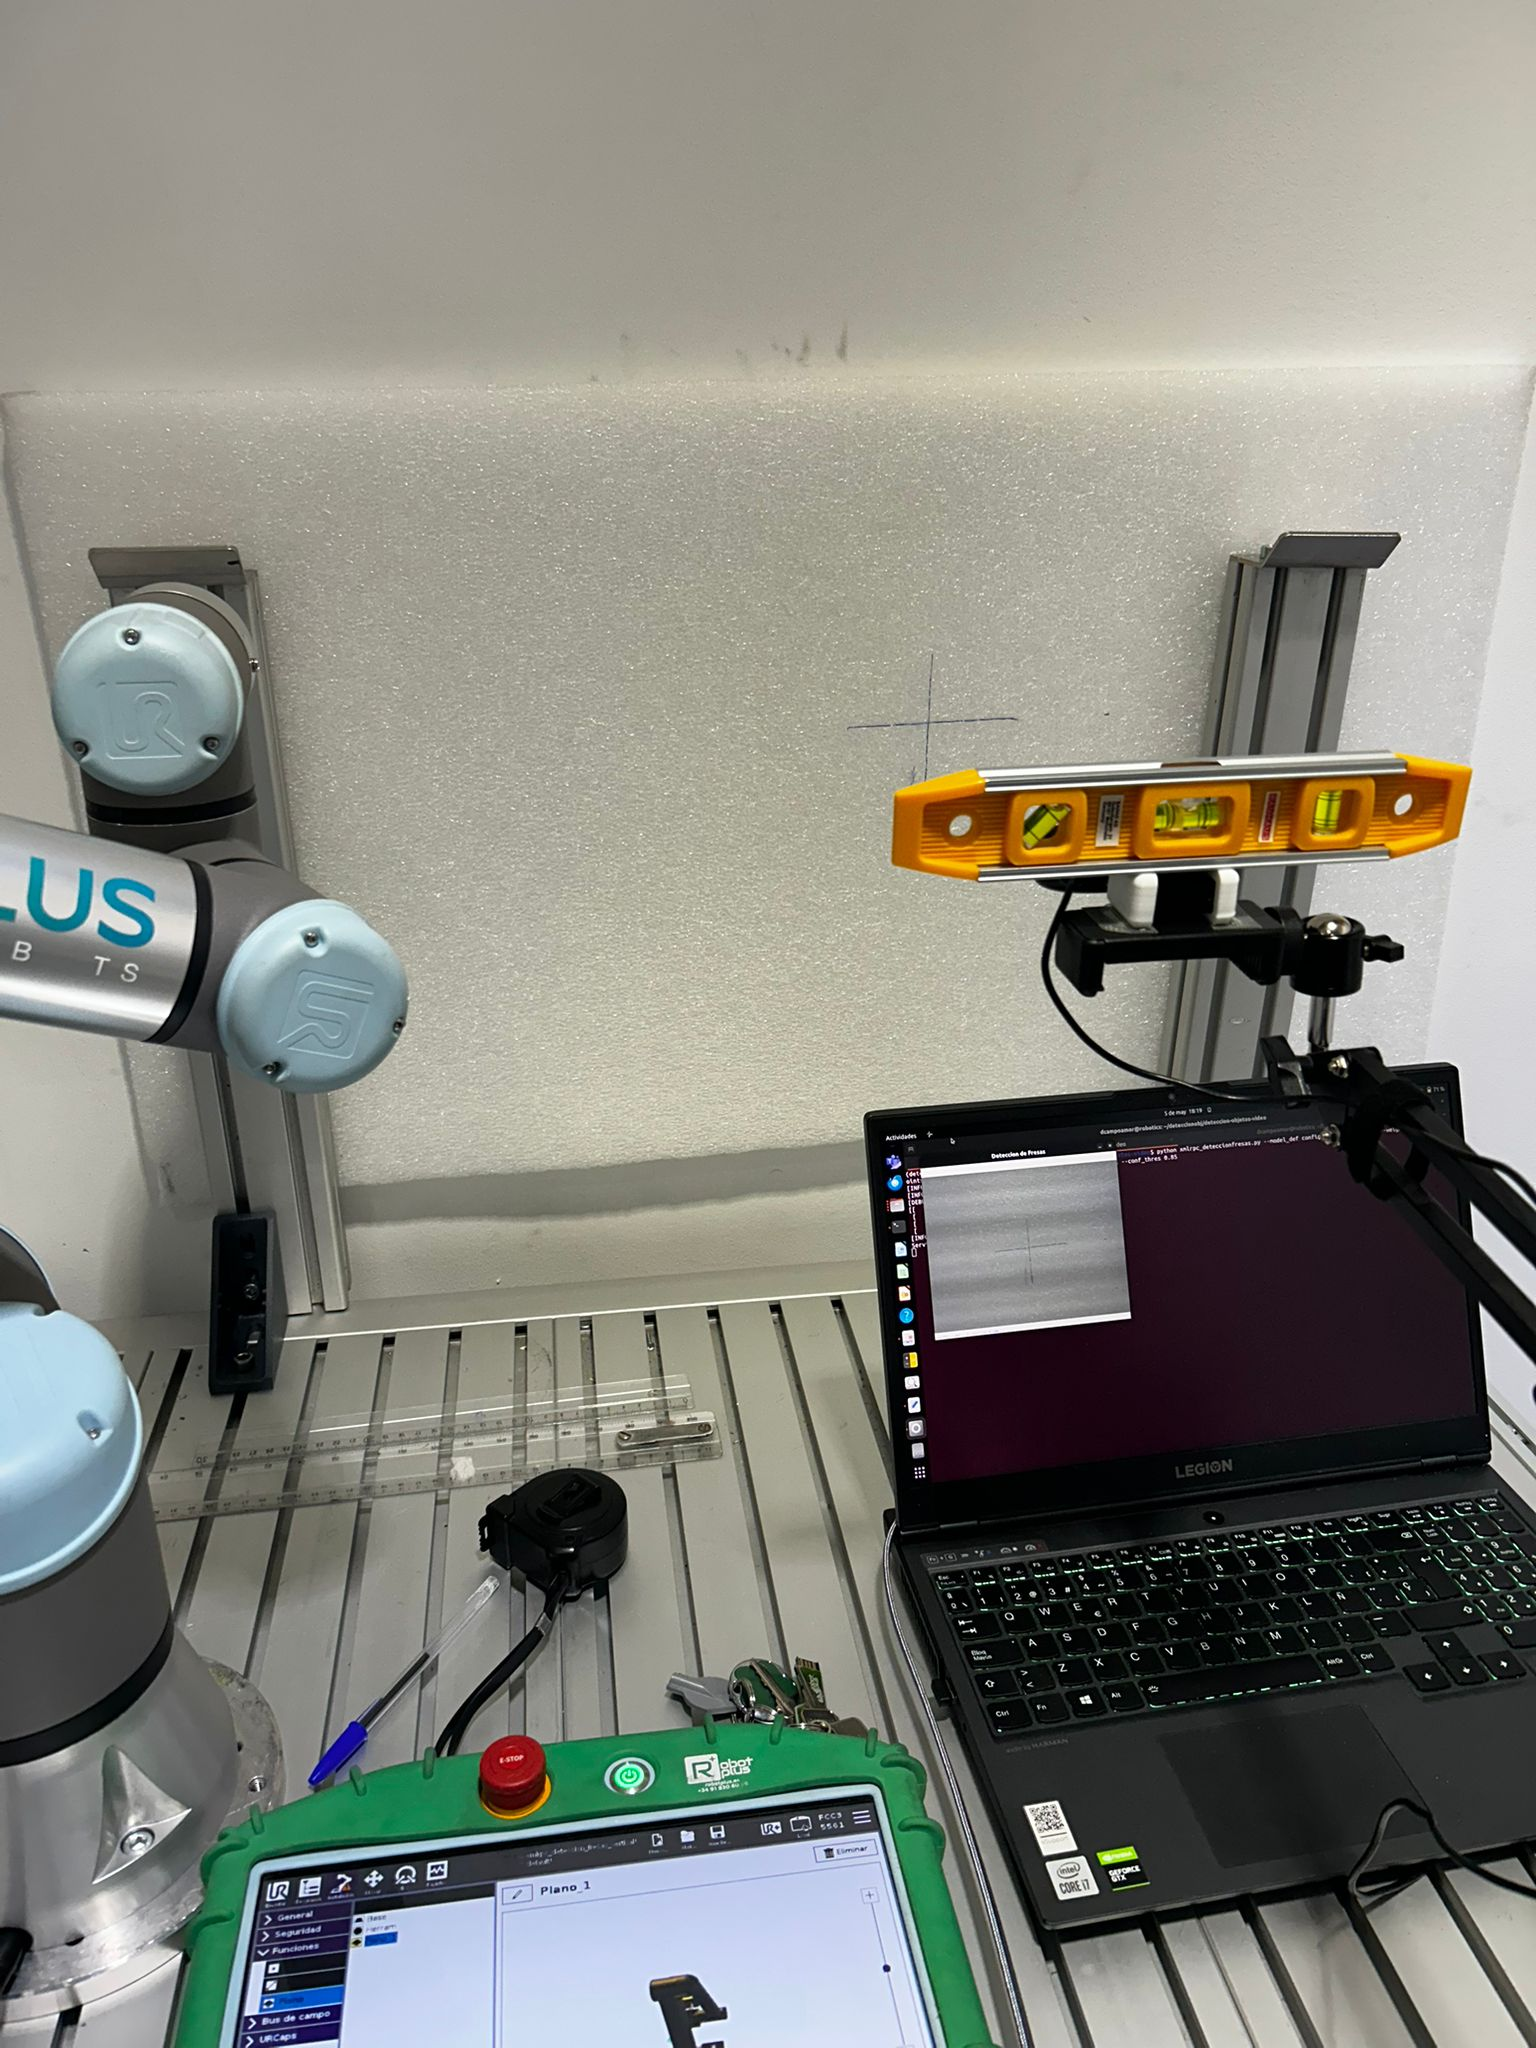
\includegraphics[width=9cm]{figs/Set up coordenadas pruebas plano vertical UR5e_3.jpeg}
    \end{center}
    \caption{Montaje del sistema final con un UR5e}
    \label{fig:montaje_final}
\end{figure}
  

\section{Hipótesis suelo adaptada al plano vertical}
\label{sec:HS_vertical}

En el sistema propuesto, la estimación de coordenadas tridimensionales se basa en la hipótesis suelo, y se realiza a partir de una única cámara estenopeica RGB fija para poder realizar esta estimación sin recurrir a sensores adicionales. Esta técnica de simplificación empleada en visión por ordenador, asume que los objetos de interés se encuentran sobre un plano conocido y fijo respecto a la cámara.\\

La hipótesis suelo (Figura \ref{fig:HS} tomada del artículo \cite{Vega21}) supone que todos los objetos del mundo en 3D están apoyados sobre el suelo, por lo tanto, asumiendo que el suelo está en el plano Z = 0, nos permitirá estimar, con el uso de la cámara, la posición 3D de los puntos que estén en el suelo.

\begin{figure} [H]
    \begin{center}
      \includegraphics[width=9cm]{figs/Hipotesis suelo.png}
    \end{center}
    \caption{La hipótesis suelo asume que todos los objetos están en el suelo}
    \label{fig:HS}
\end{figure}

El hecho de que la cámara siga el modelo \textit{pinhole} o estenopeico, implica que la proyección de un punto en el espacio bidimensional de una imagen al tridimensional se realiza usando los parámetros intrínsecos de la propia cámara y parámetros extrínsecos como la rotación o la traslación de la misma (Cuadro \ref{tab:parametros_camara}). Al asumir que los puntos están sobre el plano Z=0 mediante la hipótesis suelo, este modelo estenopeico permite estimar las coordenadas X e Y reales a partir de la imagen captada por la cámara mediante una serie de fórmulas matemáticas (Ecuación \ref{ec:formulas_pinhole}).

 \begin{table}[H]
    \centering
    \begin{tabular}{cl}
      \toprule
      \textbf{Parámetros de cámara} & \textbf{Definición} \\
      \midrule
       K (3 × 3)   & Parámetros intrínsecos \\
       R (3 × 3)   & Rotación de la cámara \\
       T (3 × 1)   & Traslación de la cámara \\
      \bottomrule
    \end{tabular}
    \caption{Definición de los parámetros de posición y orientación de la cámara pinhole}
    \label{tab:parametros_camara}
  \end{table}
  
  \begin{myequation}[H]
    \begin{align} 
       w \cdot \begin{bmatrix} u \\ v \\ 1 \end{bmatrix}
       =
       K \cdot [R \,| \, T] \cdot \begin{bmatrix} X \\ Y \\ Z \\ 1 
    \end{bmatrix}
    \nonumber
    \end{align}
    \caption{Relación de fórmulas del modelo de cámara estenopeico}
    \label{ec:formulas_pinhole}
  \end{myequation}

En esta ecuación se observa la relación entre un punto tridimensional \((X, Y, Z)\) y su proyección bidimensional \((u, v)\) multiplicada por un factor de escala \(w\) que representa la profundidad del punto proyectado en la imagen captada por la cámara, donde la matriz de parámetros instrínsecos K (Ecuación \ref{ec:matriz_intrinsecos}) junto con las matrices de rotación R (Ecuación \ref{ec:rotacion_ejes}) y la matriz de traslación T de la cámara (Ecuación \ref{ec:matriz_traslacion}), constituyen la matriz de proyección. Esta matriz de proyección transforma los puntos tridimensionales al plano imagen. 

  \begin{myequation}[H]
    \begin{align}
      K = 
      \begin{pmatrix}
        F_x & 0   & C_x \\
        0   & F_y & C_y \\
        0   & 0   & 1
      \end{pmatrix}
      \nonumber
    \end{align}
    \caption{Matriz de parámetros intrínsecos de la cámara}
    \label{ec:matriz_intrinsecos}
  \end{myequation}

  \begin{myequation}[H]
    \begin{align*}
      R(\theta)_X &= 
      \begin{pmatrix}
        1 & 0 & 0 \\
        0 & \cos(\theta) & \sin(\theta) \\
        0 & -\sin(\theta) & \cos(\theta)
      \end{pmatrix} \\[2ex]
      \nonumber
      R(\theta)_Y &= 
      \begin{pmatrix}
        \cos(\theta) & 0 & -\sin(\theta) \\
        0 & 1 & 0 \\
        \sin(\theta) & 0 & \cos(\theta)
      \end{pmatrix} \\[2ex]
      \nonumber
      R(\theta)_Z &= 
      \begin{pmatrix}
        \cos(\theta) & -\sin(\theta) & 0 \\
        \sin(\theta) & \cos(\theta) & 0 \\
        0 & 0 & 1
        \nonumber
      \end{pmatrix}
    \end{align*}
    \caption{Matrices de rotación \( R(\theta) \) según el eje de rotación}
    \label{ec:rotacion_ejes}
  \end{myequation}


  \begin{myequation}[H]
    \begin{align}
      T =
      \begin{pmatrix}
        t_x \\
        t_y \\
        t_z
      \end{pmatrix}
    \nonumber
    \end{align}
    \caption{Matriz de traslación de la cámara en coordenadas tridimensionales}
    \label{ec:matriz_traslacion}
  \end{myequation}


Para poder obtener la proyección tridimensional a partir de la bidimensional habría que operar en la Ecuación \ref{ec:formulas_pinhole} para despejar las incógnitas \((X, Y, Z)\), siendo la distancia a la cámara constante y conocida (\( Z = Z_0) \) debido a la hipótesis suelo (Ecuación \ref{ec:inversion_pinhole}), ya que que se dispone de los parámetros intrínsecos de la cámara y la geometría del plano.

  \begin{myequation}[H]
    \begin{align*}
      &K^{-1} \cdot w \cdot 
      \begin{bmatrix}
        u \\
        v \\
        1
      \end{bmatrix}
      =
      R \cdot 
      \begin{bmatrix}
        X \\
        Y \\
        Z_0
      \end{bmatrix}
      + T \\[2ex]
      &\begin{bmatrix}
        X \\
        Y \\
        Z_0
      \end{bmatrix}
      =
      R^{-1} \cdot 
      \left(
      K^{-1} \cdot w \cdot 
      \begin{bmatrix}
        u \\
        v \\
        1
      \end{bmatrix}
      - T
      \right)
    \end{align*}
    \caption{Descomposición e inversión parcial del modelo de cámara pinhole para estimar las coordenadas tridimensionales de un punto conocido en imagen bajo la hipótesis suelo \(Z = Z_0\).}
    \label{ec:inversion_pinhole}
  \end{myequation}

En este caso, y debido a la orientación del escenario, la hipótesis suelo ha sido adaptada al plano vertical, lo que significa que se asume que las fresas están dispuestas sobre una superficie vertical, como es el caso en los huertos verticales. En este plano de trabajo vertical, se ha establecido un sistema de coordenadas 3D cuyo origen coincide con el punto central del campo de visión de la cámara, actuando como referencia para crear el plano de trabajo en el robot a través de su interfaz y utlizando las mismas orientaciones de los ejes de coordenadas de la cámara (Figura \ref{fig:Plano_pared_UR}). Esto permite que una vez realizado el cálculo de las coordenadas de las fresas detectadas y el de las distancias a cada detección (Ecuación \ref{ec:formula_distancia}), estas coincidan con las coordenadas en este plano vertical, simplificando de esta manera el proceso de transformación de las coordenadas. 

\begin{myequation}[H]
  \begin{align}
    \text{distancia} = \sqrt{X^2 + Y^2 + Z^2}
  \nonumber
  \end{align}
\caption{Fórmula del cálculo de la distancia de la cámara a las detecciones}
\label{ec:formula_distancia}
\end{myequation}


\begin{figure} [H]
    \begin{center}
      \includegraphics[width=14cm]{figs/Plano Pared Programa UR.png}
    \end{center}
    \caption{Plano pared generado en el UR}
    \label{fig:Plano_pared_UR}
\end{figure}


\section{Deep Learning}
\label{sec:Tecnica_Vision}

La detección de las fresas maduras se ha resuelto mediante el uso de técnicas de visión artificial basadas en deep learning, concretamente, se ha utilizado el modelo YOLOv3 (You Only Look Once), un detector de objetos en tiempo real ampliamente utilizado por su equilibrio entre precisión y velocidad, tal y como se define en la Sección \ref{sec:YOLOv3}.\\

Este modelo ha sido entrenado específicamente para reconocer fresas maduras en las condiciones del entorno de trabajo, y una vez entrenado, se ha integrado en un script que analiza el flujo de vídeo en tiempo real y devuelve las coordenadas y la distancia a la cámara de cada fresa detectada en la imagen, junto con la clase del objeto y la confianza de detección (Figura \ref{fig:deteccion_dl}).\\

Para mejorar la precisión a la hora de estimar la posición de la fresa, se ha utilizado el centro del \textit{bounding box} de la fresa detectada como punto de referencia para la proyección sobre el plano vertical, conforme a la hipótesis descrita en la Sección \ref{sec:HS_vertical}.\\

\begin{figure} [H]
    \begin{center}
      \includegraphics[width=15cm]{figs/POV Camara Pruebas plano vertical deteccion multiple UR5e.png}
    \end{center}
    \caption{Detección de fresas maduras mediante deep learning}
    \label{fig:deteccion_dl}
\end{figure}

\section{Arquitectura del sistema}
\label{sec:arquitectura_sistema}

El prototipo final se ha implementado utilizando una combinación de componentes hardware y software específicamente seleccionados y configurados para responder a los requisitos del sistema de recolección automatizada descritos con detalle en el Capítulo \ref{cap:capitulo4}. Esta integración ha sido diseñada para garantizar la detección precisa de fresas, el cálculo de su localización espacial en coordenadas tridimensionales y la ejecución del movimiento del robot sobre estas posiciones (Figura \ref{fig:UR5e_planopared}). 

  \begin{figure}[H]
      \begin{center}
        \subcapcentertrue
        \subfigure[Detección simple en el plano vertical]{\includegraphics[width=65mm]{figs/Pruebas plano vertical deteccion simple UR5e.jpeg}}
        \hspace{1mm}
        \subfigure[Detección múltiple en el plano vertical]{\includegraphics[width=65mm]{figs/Pruebas plano vertical deteccion multiple UR5e.jpeg}}
      \end{center}
      \caption{Disposición de las detecciones para un plano horizontal con un UR5e}
      \label{fig:UR5e_planopared}
   \end{figure}

A partir de esta base, este apartado expone el proceso completo de integración y funcionamiento coordinado de los distintos módulos que conforman la solución propuesta, siendo este el siguiente:

\begin{itemize}
  \item La cámara captura imágenes de la escena en tiempo real.
  \item El modelo de deep learning detecta las fresas maduras y genera sus posiciones en píxeles gracias al fragmento de código del script en Python \ref{cod:dp_pixeles}.    
    \begin{code}[H]
      \begin{lstlisting}[language=Python] 
         with torch.no_grad():
              detections = model(imgTensor)
              detections = non_max_suppression(detections, opt.conf_thres, opt.nms_thres)

         positions = []
         if detections:
            for detection in detections:
                if detection is not None:
                   detection = rescale_boxes(detection, opt.img_size, frame.shape[:2])
                   for i, det in enumerate(detection):
                       if len(det) == 7:  
                           x1, y1, x2, y2, cls_conf, conf, cls_pred = det
                           box_w = x2 - x1
                           box_h = y2 - y1
                           center_x = x1 + box_w // 2
                           center_y = y1 + box_h // 2
                           color = (255, 0, 0)
                           cv2.rectangle(frame, (int(x1), int(y1)), (int(x2), int(y2)), color, 2)
                           label = f"Fresa - P{i+1}"
                           cv2.putText(frame, label, (int(x1), int(y1) - 10),
                                       cv2.FONT_HERSHEY_SIMPLEX, 0.5, color, 2)
                           confidence_text = f"{float(cls_conf):.2f}"
                           cv2.putText(frame, confidence_text, (int(x2) + 10, int(y1)),
                                       cv2.FONT_HERSHEY_SIMPLEX, 0.5, color, 2)
                           p2d = np.array([center_x, center_y])            
      \end{lstlisting}
      \caption{Fragmento del código que permite que el modelo de \textit{deep learning} detecte las fresas maduras y genere sus posiciones en píxeles}
      \label{cod:dp_pixeles}
    \end{code}

  \item Estas coordenadas se proyectan al espacio tridimensional sobre el plano vertical utilizando la función \texttt{getIntersectionZ(p2d)} (Código \ref{cod:getIntersectionZ}), que calcula la intersección del rayo proyectado con el plano Z definido por la posición de la cámara utlizando como argumento de entrada \texttt{p2d}, es decir, las coordenadas en píxeles de la detección (Código \ref{cod:2D_a_3D}).
 
    \begin{code}[H]
      \begin{lstlisting}[language=Python] 
                           pixelOnGround3D = getIntersectionZ(p2d)
                           x_punto = float(pixelOnGround3D[0])
                           y_punto = float(pixelOnGround3D[1])
                           z_punto = float(pixelOnGround3D[2])
                           positions.append((x_punto, y_punto, z_punto)) 
      \end{lstlisting}
      \caption{Fragmento del código que realiza la retroproyección desde 2D a 3D}
      \label{cod:2D_a_3D}
    \end{code}                   
       
    \begin{code}[H]
      \begin{lstlisting}[language=Python]      
      def getIntersectionZ(p2d):
           p2d_h = np.array([p2d[0], p2d[1], 1])
           inv_K = np.linalg.inv(myCamera.k[:, :3])
           inv_RT = np.linalg.inv(myCamera.rt[:3, :3])
           p3d_h = np.dot(inv_K, p2d_h)
           p3d_h = np.dot(inv_RT, p3d_h)
           if np.abs(p3d_h[2]) > 1e-6:
               escala = -myCamera.position[2] / p3d_h[2]
               p3d_h *= escala
           return np.array(p3d_h)
      \end{lstlisting}
      \caption{Función \texttt{getIntersecionZ()}}
      \label{cod:getIntersectionZ}
    \end{code}                                    
                           
  \item El servidor XML-RPC se crea en la dirección IP y puerto especificado, se transmiten las coordenadas al robot a través de la función \texttt{get\_next\_pose()}, y lanza en un hilo independiente que queda a la espera de nuevas peticiones (Código \ref{cod:get_next_pose}).
  
    \begin{code}[H]
      \begin{lstlisting}[language=Python] 
      # Conexion con el robot usando XML-RPC
      server = SimpleXMLRPCServer(("192.168.23.107", 50000))
      server.RequestHandlerClass.protocol_version = "HTTP/1.1"
      print("Servidor XML-RPC corriendo en el puerto 50000...")
      
      def get_next_pose():
          if detected_points:
              pose = detected_points[-1]
              print(f"[DEBUG] Enviando ultima posicion detectada: {pose}")
              return [pose[0], pose[1], pose[2], 0, 0, 0]
          else:
              print(f"[DEBUG] No se detectaron puntos, enviando posicion de inicio")
              return [0, 0, 0, 0, 0, 0]

      server.register_function(get_next_pose, "get_next_pose")
      import threading
      server_thread = threading.Thread(target=server.serve_forever)
      server_thread.daemon = True
      server_thread.start()
      \end{lstlisting}
      \caption{Envío de la última posición tridimensional detectada al robot mediante XML-RPC}
      \label{cod:get_next_pose}
    \end{code}          
  
  \item El robot interpreta la posición, calcula una trayectoria y actúa sobre la fruta detectada (Figura \ref{fig:Config_comunicación_UR}).
    \begin{figure}[H]
      \begin{center}
        \subcapcentertrue
        \subfigure[Configuración de la comunicación XMLRPC en el robot]{\includegraphics[width=72mm]{figs/Antes de Iniciar_XMLRPC.png}}
        \hspace{4mm}
        \subfigure[Instrucciones de movimiento del robot según la casuística]{\includegraphics[width=72mm]{figs/Movimiento UR.png}}
      \end{center}
      \caption{Ajustes de comunicación XMLRPC en el robot y ejecución de movimientos definidos en el programa}
      \label{fig:Config_comunicación_UR}
    \end{figure}
 
\end{itemize}

Esta arquitectura permite un sistema modular, robusto y fácilmente escalable a escenarios reales más complejos, sentando las bases para su posible aplicación futura en entornos agrícolas reales o semiautomatizados. Para hacer funcionar el sistema completo y conseguir una correcta integración entre el sistema de visión y el brazo robótico UR, deben seguirse los siguientes pasos de forma ordenada.

\begin{enumerate}
  \item Conexión de red: En primer lugar, es fundamental asegurarse de que, tanto el robot como el ordenador que ejecuta el sistema de visión, están conectados a la misma red local y que ambos dispositivos pertenezcan a la misma subred, y se recomienda usar conexión por cable para mayor estabilidad. Es necesario comprobar que hay conectividad entre ambos dispositivos (por ejemplo, mediante un ping a la IP del robot desde el ordenador), ya que la comunicación se establece a través del protocolo XML-RPC sobre una dirección IP y puerto determinados.
    
      \begin{figure} [H]
        \begin{center}
          \includegraphics[width=90mm]{figs/Ajustes de Red UR.png}
        \end{center}
        \caption{Ajustes de red en el robot}
        \label{fig:ajustes_red_UR}
      \end{figure} 
  
  \item Definición de la Instalación del robot: Si el robot lleva instalado un efector final, como una garra o un actuador, es importante configurar correctamente la carga útil, el peso y el centro de gravedad en el software del UR, ya que esto garantiza un funcionamiento seguro y preciso, ajustando los parámetros de control de movimiento y compensación de la cinemática.
  
    \begin{figure}[H]
      \begin{center}
        \subcapcentertrue
        \subfigure[Configuración del Punto Central de la Herramienta (PCH)]{\includegraphics[width=72mm]{figs/Config_PCH.png}}
        \hspace{4mm}
        \subfigure[Configuración de la carga]{\includegraphics[width=72mm]{figs/config_Carga.png}}
      \end{center}
      \caption{Definición de la Instalación del efector final en el robot}
      \label{fig:Config_UR}
    \end{figure}
  
  \item Creación del plano de trabajo: A continuación, se debe definir el plano de trabajo sobre el que se va a operar, en este caso un plano vertical, como se detalló en la Sección \ref{sec:HS_vertical}. 
  
  \item Lanzamiento del sistema de comunicación: En este punto, se debe ejecutar el script en Python, tal y como muestra la Figura \ref{fig:ejecucion_python}. Para este caso, es el programa \textit{xmlrpc\_deteccionfresas.py}\footnote{\url{https://github.com/RoboticsURJC/tfg-dcampoamor/blob/main/src/robot/xmlrpc_deteccionfresas.py}} el que ejerce de servidor, y tiene que ejecutarse desde la terminal del ordenador para poder ejecutar posteriormente mediante el botón de \textit{play} de la interfaz del robot, el programa \textit{xmlrpc\_deteccion\_fresas\_vertical.urp}\footnote{\url{https://github.com/RoboticsURJC/tfg-dcampoamor/blob/main/src/robot/xmlrpc_deteccion_fresas_vertical.urp}}, que realiza la solicitud de datos al servidor remoto a través del protocolo XML-RPC, una vez que el servidor esté en marcha.
  
    \begin{figure} [H]
        \begin{center}
          \includegraphics[width=135mm]{figs/Ejecutar_Programa_Python.png}
        \end{center}
        \caption{Lanzamiento del servidor mediante el programa en Python en la terminal del ordenador}
        \label{fig:ejecucion_python}
    \end{figure} 
  
  \item Ejecución: Una vez en marcha tanto el programa en el ordenador como en el robot, el sistema detectará automáticamente las fresas presentes en la escena, calculará sus coordenadas tridimensionales y las enviará al robot, que ejecutará el movimiento correspondiente según el programa \textit{xmlrpc\_deteccion\_fresas\_vertical.urp}\footnote{\url{https://github.com/RoboticsURJC/tfg-dcampoamor/blob/main/src/robot/xmlrpc_deteccion_fresas_vertical.urp}} para acercarse al fruto y proceder a su recolección.
      
    \begin{figure}[H]
      \begin{center}
        \subcapcentertrue
        \subfigure[Ejecución del programa en Python en la terminal del ordenador]{\includegraphics[width=78mm]{figs/POV Camara Pruebas plano vetical deteccion simple UR5e}}
        \hspace{4mm}
        \subfigure[Ejecución del programa de robot]{\includegraphics[width=70mm]{figs/Carpetas del Programa UR.png}}
      \end{center}
      \caption{Ejecución de los programas de manera simultánea}
      \label{fig:Ejecucion_programas}
    \end{figure}
\end{enumerate}

Para completar la evaluación del prototipo, a pesar de que no se llegó a implementar la acción de cierre o agarre de la pinza dentro del flujo automatizado del sistema, se realizaron pruebas complementarias utilizando una pinza industrial acoplada al robot en el programa de robot \textit{xmlrpc\_deteccion\_fresas\_vertical\_pinza.urp}\footnote{\url{https://github.com/RoboticsURJC/tfg-dcampoamor/blob/main/src/robot/xmlrpc_deteccion_fresas_vertical_pinza.urp}} (Figura \ref{fig:Programa_UR_pinza}) con el objetivo de verificar la compatibilidad y robustez del programa desarrollado que permitieron demostrar que el sistema era plenamente funcional y adaptable, y que se podía integrar sin inconvenientes cualquier herramienta de agarre que sea adecuada para el manejo de fresas, dada su delicadeza. De este modo, se confirma que el sistema de detección, proyección y comunicación con el robot puede extenderse fácilmente para incluir un actuador final destinado a la recolección efectiva del fruto en un entorno real (Figura \ref{fig:UR5e_planopared_garra}).

   \begin{figure}[H]
      \begin{center}
        \subcapcentertrue
        \subfigure{\includegraphics[width=69mm]{figs/Antes de Iniciar Programa UR Pinza.png}}
        \hspace{1mm}
        \subfigure{\includegraphics[width=69mm]{figs/Movimiento UR Programa UR Pinza.png}}
      \end{center}
      \caption{Programa \textit{xmlrpc\_deteccion\_fresas\_vertical\_pinza.urp} para uso del sistema con efector final}
      \label{fig:Programa_UR_pinza}
   \end{figure}
   
   
   \begin{figure}[H]
      \begin{center}
        \subcapcentertrue
        \subfigure{\includegraphics[width=69mm]{figs/Pruebas plano vertical deteccion simple garra UR5e.jpeg}}
        \hspace{1mm}
        \subfigure{\includegraphics[width=65mm]{figs/Pruebas plano vertical deteccion simple garra UR5e_2.png}}
      \end{center}
      \caption{Pruebas en el plano vertical de detección con garra integrada}
      \label{fig:UR5e_planopared_garra}
   \end{figure}


\pagebreak

Con todo lo anterior, se ha descrito en detalle el sistema desarrollado, incluyendo los fundamentos técnicos, las herramientas de visión artificial empleadas, y el proceso de integración con el robot colaborativo UR, siendo un sistema diseñado con el objetivo de ser modular, reproducible y eficaz en tareas de detección y recolección de frutos maduros en entornos controlados. En el Anexo \ref{cap:capitulo7}, se presentan los experimentos realizados, donde se detallan las diferentes pruebas llevadas a cabo, los ajustes realizados durante el desarrollo y los resultados obtenidos hasta alcanzar el estado funcional final del proyecto.



















\setlength{\parskip}{0.7em} % Espaciado vertical entre p�rrafos
\chapter{Conclusiones}
\label{cap:capitulo5}

\begin{flushright}
\begin{minipage}[]{10cm}
\emph{Quizás algún fragmento de libro inspirador...}\\
\end{minipage}\\

Autor, \textit{Título}\\
\end{flushright}

\vspace{1cm}

Escribe aquí un párrafo explicando brevemente lo que vas a contar en este capítulo, que básicamente será una recapitulación de los problemas que has abordado, las soluciones que has prouesto, así como los experimentos llevados a cabo para validarlos. Y con esto, cierras la memoria.

\section{Conclusiones}

Enumera los objetivos y cómo los has cumplido.\\

Enumera también los requisitos implícitos en la consecución de esos objetivos, y cómo se han satisfecho.\\

No olvides dedicar un par de párrafos para hacer un balance global de qué has conseguido, y por qué es un avance respecto a lo que tenías inicialmente. Haz mención expresa de alguna limitación o peculiaridad de tu sistema y por qué es así. Y también, qué has aprendido desarrollando este trabajo.\\

Por último, añade otro par de párrafos de líneas futuras; esto es, cómo se puede continuar tu trabajo para abarcar una solución más amplia, o qué otras ramas de la investigación podrían seguirse partiendo de este trabajo, o cómo se podría mejorar para conseguir una aplicación real de este desarrollo (si es que no se ha llegado a conseguir).

\section{Corrector ortográfico}

Una vez tengas todo, no olvides pasar el corrector ortográfico de \LaTeX a todos tus ficheros \textit{.tex}. En \texttt{Windows}, el propio editor \texttt{TeXworks} incluye el corrector. En \texttt{Linux}, usa \texttt{aspell} ejecutando el siguiente comando en tu terminal:

\begin{verbatim}
aspell --lang=es --mode=tex check capitulo1.tex
\end{verbatim}



\clearpage
\thispagestyle{empty}

\printindex %\nocite{*}

\appendix
\renewcommand{\thechapter}{\Roman{chapter}}

%Inicia la secci�n de ap�ndices
\setlength{\parskip}{0.7em} % Espaciado vertical entre p�rrafos
\chapter{Conclusiones}
\label{cap:capitulo7}

\begin{flushright}
\begin{minipage}[]{10cm}
\emph{Quizás algún fragmento de libro inspirador...}\\
\end{minipage}\\

Autor, \textit{Título}\\
\end{flushright}

\vspace{1cm}

Escribe aquí un párrafo explicando brevemente lo que vas a contar en este capítulo, que básicamente será una recapitulación de los problemas que has abordado, las soluciones que has prouesto, así como los experimentos llevados a cabo para validarlos. Y con esto, cierras la memoria.

\section{Conclusiones}

Enumera los objetivos y cómo los has cumplido.\\

Enumera también los requisitos implícitos en la consecución de esos objetivos, y cómo se han satisfecho.\\

No olvides dedicar un par de párrafos para hacer un balance global de qué has conseguido, y por qué es un avance respecto a lo que tenías inicialmente. Haz mención expresa de alguna limitación o peculiaridad de tu sistema y por qué es así. Y también, qué has aprendido desarrollando este trabajo.\\

Por último, añade otro par de párrafos de líneas futuras; esto es, cómo se puede continuar tu trabajo para abarcar una solución más amplia, o qué otras ramas de la investigación podrían seguirse partiendo de este trabajo, o cómo se podría mejorar para conseguir una aplicación real de este desarrollo (si es que no se ha llegado a conseguir).

\section{Corrector ortográfico}

Una vez tengas todo, no olvides pasar el corrector ortográfico de \LaTeX a todos tus ficheros \textit{.tex}. En \texttt{Windows}, el propio editor \texttt{TeXworks} incluye el corrector. En \texttt{Linux}, usa \texttt{aspell} ejecutando el siguiente comando en tu terminal:

\begin{verbatim}
aspell --lang=es --mode=tex check capitulo1.tex
\end{verbatim}



\setlength{\parskip}{0.7em} % Espaciado vertical entre p�rrafos
\chapter{Experimentos}
\label{cap:capitulo8}

En este apéndice se recogen las distintos experimentos que se han llevado a cabo durante el desarrollo del proyecto. Estas pruebas han sido fundamentales para verificar el correcto funcionamiento del sistema de reconocimiento de fresas maduras y su comunicación con el brazo robótico, permitiendo así alcanzar los objetivos definidos en fases anteriores del trabajo.

\section{Detección con YOLOv3 y TensorFlow}
\label{exp_seleccion_algoritmo}

Dada la finalidad del proyecto, se requería que la detección de objetos se diera en tiempo real, por lo que se buscó información sobre YOLO, un sistema de código abierto que permitía esto a partir de una red neuronal convolucional para detectar objetos en imágenes y vídeo. De este modo se iniciaron las pruebas pertinentes para la selección del algoritmo de detección y de las bibliotecas a utilizar.

\subsection{Pruebas con imágenes}
\label{sec:Pruebas_imgs_TF}

En primer lugar, se creó un entorno de Anaconda para poder probar la detección de objetos en imágenes utilizando Tensorflow mediante el repositorio \verb|deteccion_objetos|\footnote{\url{https://github.com/puigalex/deteccion_objetos}}, que estaba basado en la configuración \verb|faster rcnn resnet101 coco| como modelo de detección de objetos. Se llevó a cabo el etiquetado de imágenes, en este caso de tigres, mediante la herramienta labelImg\footnote{\url{https://github.com/HumanSignal/labelImg}}, y se prepararon las carpetas y archivos de configuración correspondientes para poder llevar a cabo el entrenamiento del modelo, siguiendo los pasos indicados en el repositorio; y utilizando una distribución de las imágenes utilizadas para el aprendizaje del modelo y su uso en la detección aproximadamente del 70:30 (73\% datos de entrenamiento y 27\% datos de prueba)(Cuadro \ref{tab:Imagenes_Entrenamiento}), a partir de los cuales se entrenó ese 70\% con uno de los algoritmos y los respectivos parámetros escogidos, y medimos su rendimiento usando el 30\% restante de los datos.\\

  \begin{table}[H]
  \centering
  \begin{tabularx}{\textwidth}{|X|X|X|}
    \hline
    \centering \textbf{Imágenes usadas en entrenamiento} & 
    \centering \textbf{Imágenes usadas en test} & 
    \centering \textbf{Número total de imágenes} \tabularnewline
    \hline
    \centering 594 & \centering 218 & \centering 812 \tabularnewline
    \hline
  \end{tabularx}
  \caption{Distribución de las imágenes utilizadas para el entrenamiento del modelo}
  \label{tab:Imagenes_Entrenamiento}
  \end{table}

Se entrenó este modelo hasta que se observó que la pérdida estaba por debajo de 1, considerando que esta pérdida no era alta, y que no existían demasiadas fluctuaciones,  deteniendo este entrenamiento a los 1400 pasos, a pesar de que este entrenamiento estaba programado para llegar hasta los 20000. Esto supuso que se tuviera que utilizar el último checkpoint disponible, en este caso el del paso 1337, %(Figura \ref{fig:Deteccion_Prueba_TF}), 
para convertirlo en un modelo final y de esta manera poder generar predicciones, utilizando imágenes de diferentes tamaños.

  %\begin{figure}[H]
  %  \begin{center}
  %    \subcapcentertrue
  %    \subfigure[Pasos finales del entrenamiento con TensorFlow]{\includegraphics[height=50mm, width=70mm]{figs/Pasos finales del entrenamiento_TF.png}}
  %    \hspace{4mm}
  %    \subfigure[Checkpoints del entrenamiento con TensorFlow]{\includegraphics[height=50mm, width=70mm]{figs/checkpoints_TF.png}}
  %  \end{center}
  %  \caption{Entrenamiento del algoritmo con TensorFlow}
  %  \label{fig:Deteccion_Prueba_TF}
  %\end{figure}
  
Una vez convertido el checkpoint en un modelo final, se procedió a realizar las primeras pruebas de detección en imágenes de este modelo, comprobando su capacidad para detectar correctamente los tigres en este caso, y se evaluó visualmente los resultados obtenidos en algunos ejemplos mostrados en la Figura \ref{fig:deteccion_tensorflow_tigres}.

  \begin{figure}[H]
  \centering
  % Fila 1
  \begin{minipage}{0.46\textwidth}
    \centering
    \includegraphics[width=\linewidth]{figs/tigre_1.jpeg}
  \end{minipage}
  \hspace{2mm}
  \begin{minipage}{0.46\textwidth}
    \centering
    \includegraphics[width=\linewidth]{figs/tigre_2.jpeg}
  \end{minipage}
  \\[4mm] % Espacio vertical entre las dos filas
  % Fila 2
  \begin{minipage}{0.46\textwidth}
    \centering
    \includegraphics[width=\linewidth]{figs/tigre_4.jpeg}
  \end{minipage}
  \hspace{2mm}
  \begin{minipage}{0.46\textwidth}
    \centering
    \includegraphics[width=\linewidth]{figs/tigre_5.jpeg}
  \end{minipage}
  \caption{Resultado de la detección en imágenes con TensorFlow}
  \label{fig:deteccion_tensorflow_tigres}
  \end{figure}
 
Tras los resultados obtenidos en las imágenes utilizadas para esta primera prueba, se decidió llevar a cabo un nuevo proceso de entrenamiento a partir del último checkpoint disponible, con el objetivo principal de comprobar si, aumentando el número de pasos de entrenamiento, se lograba una mejora significativa tanto en la disminución del valor de pérdida, como en el incremento del porcentaje de confianza en las detecciones realizadas.
Así, se retomó el entrenamiento desde el checkpoint del paso 1337, extendiéndose en esta segunda ocasión hasta el paso 2945, momento en el cual se optó por detener manualmente el proceso al observarse una estabilización progresiva en los valores de pérdida, y siendo el último checkpoint generado el correspondiente al paso 2877, obteniéndose en este punto un valor de pérdida de tan solo 0.222, notablemente inferior al registrado en el primer intento. 

A continuación, se procedió a ejecutar nuevamente el programa sobre las mismas imágenes de prueba de tigres empleadas en la primera serie de tests, lo que permitió realizar una comparación directa entre ambos modelos, y observar que en esta segunda ejecución existía una clara mejora en la calidad de las detecciones, tanto en términos de mayor porcentaje de confianza como en la precisión de los cuadros delimitadores sobre los objetos detectados (ver Figura \ref{fig:deteccion_tensorflow_tigres_v2}).

  \begin{figure}[H]
  \centering
  % Fila 1
  \begin{minipage}{0.46\textwidth}
    \centering
    \includegraphics[width=\linewidth]{figs/tigre_1_v2.jpeg}
  \end{minipage}
  \hspace{2mm}
  \begin{minipage}{0.46\textwidth}
    \centering
    \includegraphics[width=\linewidth]{figs/tigre_2_v2.jpeg}
  \end{minipage}
  \\[4mm] % Espacio vertical entre las dos filas
  % Fila 2
  \begin{minipage}{0.46\textwidth}
    \centering
    \includegraphics[width=\linewidth]{figs/tigre_4_v2.jpeg}
  \end{minipage}
  \hspace{2mm}
  \begin{minipage}{0.46\textwidth}
    \centering
    \includegraphics[width=\linewidth]{figs/tigre_5_v2.jpeg}
  \end{minipage}
  \caption{Resultado del reentrenamiento de la detección en imágenes con TensorFlow}
  \label{fig:deteccion_tensorflow_tigres_v2}
  \end{figure}

\pagebreak
Después de llevar a cabo estas pruebas con imágenes de tigres, se comprobó que el modelo funcionase también con fresas, por lo que, a través de la página Kaggle, se obtuvo un dataset de 262 frutas\footnote{\url{https://www.kaggle.com/datasets/aelchimminut/fruits262}}, de las cuales únicamente se utilizó el archivo de las fresas, que contenía 1002 imágenes.

Una vez descargado el archivo, se comenzó a etiquetar una a una las imágenes mediante la herramienta labelImg para obtener los archivos xml, tal y como se había hecho con el ejemplo anterior de los tigres, y antes de terminar de etiquetar el dataset entero, se probó este modelo utilizando las primeras 405 imágenes etiquetadas siguiendo una distribución de estas del 80:20 para su entrenamiento y usando el checkpoint guardado en el paso 3490 para congelar el modelo, y así poder utilizar varias imágenes aún por etiquetar para probarlo, obteniendo un resultado satisfactorio en cuanto a la detección y su confianza, tal y como se puede observar en la Figura \ref{fig:Deteccion_Fresas_Imagenes_TF}.

  \begin{figure}[H]
  \centering
  % Fila 1
  \begin{minipage}{0.45\textwidth}
    \centering
    \includegraphics[width=\linewidth]{figs/999.jpeg}
  \end{minipage}
  \hspace{2mm}
  \begin{minipage}{0.45\textwidth}
    \centering
    \includegraphics[width=\linewidth]{figs/947.jpeg}
  \end{minipage}
  \\[4mm] % Espacio vertical entre las dos filas
  % Fila 2
  \begin{minipage}{0.45\textwidth}
    \centering
    \includegraphics[width=\linewidth]{figs/868.jpeg}
  \end{minipage}
  \hspace{2mm}
  \begin{minipage}{0.45\textwidth}
    \centering
    \includegraphics[width=\linewidth]{figs/1000.jpeg}
  \end{minipage}
  \caption{Pruebas de detección de fresas en imágenes con TensorFlow}
  \label{fig:Deteccion_Fresas_Imagenes_TF}
  \end{figure}

Tras haber conseguido la detección de fresas en imágenes estáticas utilizando TensorFlow, el siguiente paso dentro del desarrollo del sistema consistió en extender las pruebas a la detección en vídeo en tiempo real, por lo que, se procedió a evaluar distintos modelos de detección de objetos ya preentrenados sobre conjuntos de datos de referencia, lo que permitió llevar a cabo una comparación de estos diferentes modelos o sistemas bajo las mismas condiciones iniciales sin necesidad de realizar un nuevo entrenamiento desde cero. 

\subsection{Pruebas con vídeo en tiempo real}
\label{sec:Pruebas_video_TF}

Para la realización de estas pruebas, se utilizó tanto la cámara web integrada del ordenador portátil como una imagen previamente seleccionada, para que, de esta manera pudieran observarse las diferencias entre los modelos tanto en la detección en vídeo como en la detección en imágenes, y poder valorar qué modelo de los tres distintos probados ofrecería mejores prestaciones en términos de precisión, velocidad de procesamiento y robustez frente a las condiciones reales de trabajo (ver figuras  \ref{fig:modelo_ssd_mobilenet}, \ref{fig:modelo_efficientdet_d4} y \ref{fig:modelo_faster_rcnn_resnet50}). 

	\begin{figure}[H]
    		\begin{center}
      		\subcapcentertrue
      		\subfigure[Resultado del modelo en imagen]{\includegraphics[height=50mm, width=70mm]{figs/ssd_mobilenet_v2_320x320_coco17_tpu-8.jpeg}}
      		\hspace{2mm}
      		\subfigure[Resultado del modelo en vídeo]{\includegraphics[height=50mm, width=70mm]{figs/webcam ssd_mobilenet_v2_320x320_coco17_tpu-8.png}}
    	\end{center}
    	\caption{Modelo \texttt{ssd\_mobilenet\_v2\_320x320\_coco17\_tpu-8}}
    	\label{fig:modelo_ssd_mobilenet}
  	\end{figure}
  	

  	\begin{figure}[H]
    		\begin{center}
      		\subcapcentertrue
      		\subfigure[Resultado del modelo en imagen]{\includegraphics[height=50mm, width=70mm]{figs/efficientdet_d4_coco17_tpu-32.jpeg}}
      		\hspace{2mm}
      		\subfigure[Resultado del modelo en vídeo]{\includegraphics[height=50mm, width=70mm]{figs/webcam efficientdet_d4_coco17_tpu-32.png}}
    	\end{center}
    	\caption{Modelo \texttt{efficientdet\_d4\_coco17\_tpu-32}}
    	\label{fig:modelo_efficientdet_d4}
  	\end{figure}

  	\begin{figure}[H]
    		\begin{center}
      		\subcapcentertrue
      		\subfigure[Resultado del modelo en imagen]{\includegraphics[height=50mm, width=70mm]{figs/faster_rcnn_resnet50_v1_640x640_coco17_tpu-8.jpeg}}
      		\hspace{2mm}
      		\subfigure[Resultado del modelo en vídeo]{\includegraphics[height=50mm, width=70mm]{figs/webcam faster_rcnn_resnet50_v1_640x640_coco17_tpu-8.png}}
    	\end{center}
    	\caption{Modelo \texttt{faster\_rcnn\_resnet50\_v1\_640x640\_coco17\_tpu-8 }}
    	\label{fig:modelo_faster_rcnn_resnet50}
  	\end{figure}	

Después de haber llevado a cabo estas pruebas con los modelos de detección de objetos \verb|ssd_mobilenet_v2_320x320_coco17_tpu-8|, \verb|efficientdet_d4_coco17_tpu-32| y \verb|faster_rcnn_resnet50_v1_640x640_coco17_tpu-8|, y tras valorar que, el principal uso del modelo en la aplicación final sería la de llevar a cabo detecciones en tiempo real con una cámara, se escogió el modelo \verb|ssd_mobilenet_v2| para proseguir con los experimentos. 

La elección de este modelo, incluso por delante de cualquiera de los otros dos, se llevó a cabo a pesar de tener menor precisión y calidad de detección, puesto que destacaba principalmente por su elevada velocidad de procesamiento y su bajo consumo de recursos, gracias a su arquitectura ligera basada en \verb|MobileNetV2| y su tamaño de entrada reducido, haciéndolo especialmente adecuado para aplicaciones en tiempo real sobre hardware con capacidades limitadas como el implementado.

Una vez escogido el modelo, para poder llevar a cabo la detección de fresas, era necesario entrenarlo desde cero, para lo que se utilizó de guía el repositorio de GitHub \verb|real_time_object_detection_cpu|\footnote{\url{https://github.com/haroonshakeel/real_time_object_detection_cpu/blob/main}}, creando y activando un nuevo entorno de Anaconda, en el cual se instalaron los paquetes y librerías necesarios para ello, junto al Object Detection API de TensorFlow y junto con Jupyter Notebook\footnote{\url{https://jupyter.org}}, un entorno computacional interactivo basado en web para crear cuadernos que contienen código en vivo, ecuaciones, visualizaciones y texto narrativo. 

\pagebreak
Completada la configuración del entorno, la instalación de todos los componentes, y el entrenamiento del modelo, se realizó una primera prueba de detección utilizando el modelo entrenado para comprobar si funcionaba, obteniendo las primeras predicciones en tiempo real sobre vídeo con fresas reales. Estas primeras detecciones sirvieron de base para la batería de pruebas en las cuales se variaba tanto el número de fresas como las condiciones de luz, para poder conocer en qué condiciones se obtenía un mayor porcentaje de confianza en la detección (Figura \ref{fig:deteccion_Fresas_webcam_TF_ssdmobilenet}).

\begin{figure}[H]
    \centering
    \subcapcentertrue
    % Fila 1
    \subfigure[Una única fresa con luz natural de día]{\includegraphics[width=0.30\textwidth]{figs/Deteccion una fresa luz natural dia JN.png}}
    \hspace{1mm}
    \subfigure[Una única fresa con luz artificial de día]{\includegraphics[width=0.30\textwidth]{figs/Deteccion una fresa luz artificial dia JN.png}}
    \hspace{1mm}
    \subfigure[Una única fresa con luz artificial de noche]{\includegraphics[width=0.30\textwidth]{figs/Deteccion una fresa luz artificial de noche JN.png}}

    \vspace{1mm} % Espacio vertical entre filas

    % Fila 2
    \subfigure[Varias fresas con luz natural de día]{\includegraphics[width=0.30\textwidth]{figs/Deteccion varias fresas luz natural dia JN.png}}
    \hspace{1mm}
    \subfigure[Varias fresas con luz artificial de día]{\includegraphics[width=0.30\textwidth]{figs/Deteccion varias fresas luz artificial dia JN.png}}
    \hspace{1mm}
    \subfigure[Varias fresas con luz artificial de noche]{\includegraphics[width=0.30\textwidth]{figs/Deteccion varias fresas luz artificial de noche JN.png}}
    
    \caption{Detección de fresas en webcam con TensorFlow con modelos no preentrenados (\texttt{ssd mobilenet v2 320x320)}}
    \label{fig:deteccion_Fresas_webcam_TF_ssdmobilenet}
\end{figure}

Después de verificar la viabilidad y funcionamiento de estas pruebas, y de detectar en los resultados que, con luz artificial en condiciones de alta luminosidad existía un mayor porcentaje de confianza en las detecciones que con luz natural y baja luminosidad, tal y como se puede apreciar en las figuras \ref{fig:Pruebas_luminosidad} y \ref{fig:Grafica_medias_luminosidad}, se modificó el programa de detección para obtener más datos sobre estas detecciones y dotar al programa de nuevas funcionalidades.

    \begin{figure}[H]
    \begin{center}
      \subcapcentertrue
      \subfigure[Resultados de las pruebas de detección con alta luminosidad]{\includegraphics[width=125mm]{figs/Grafica deteccion alta luminosidad.png}}
      \hspace{4mm}
      \subfigure[Resultados de las pruebas de detección con baja luminosidad]{\includegraphics[width=125mm]{figs/Grafica deteccion baja luminosidad.png}}
    \end{center}
    \caption{Gráficas de la confianza de detección obtenida en las pruebas según la luminosidad para el modelo \texttt{ssd mobilenet v2}}
    \label{fig:Pruebas_luminosidad}
  \end{figure}
  
  \begin{figure}[H]
    \begin{center}
      \subcapcentertrue
      \subfigure[Porcentaje medio de confianza para las detecciones con alta luminosidad]{\includegraphics[width=70mm]{figs/Deteccion media con alta luminosidad.png}}
      \hspace{4mm}
      \subfigure[Porcentaje medio de confianza para las detecciones con baja luminosidad]{\includegraphics[width=70mm]{figs/Deteccion media con baja luminosidad.png}}
    \end{center}
    \caption{Gráficas de la media de los porcentajes de confianza obtenidos en las pruebas de detección según la luminosidad para el modelo \texttt{ssd mobilenet v2}}
    \label{fig:Grafica_medias_luminosidad}
  \end{figure}

Estas modificaciones incluían la instrucción mediante la cual se dejase de captar lo que se podía ver por la cámara del ordenador y se cerrase la ventana emergente correspondiente al finalizar la ejecución el programa, a la que también se le cambió el nombre por \textit{strawberry detection}. También se calcularon las coordenadas del punto central del recuadro de la detección, y se añadió el cálculo de los FPS (fotogramas por segundo) en tiempo real en la ventana (ver Figura \ref{fig:Coord_JN}); midiendo la velocidad de procesamiento de los cuadros, lo cuál era útil para comparar entre las distintas condiciones de detección, ya que un FPS más alto indicaba que se estaban procesando más cuadros por segundo, lo que es deseable para aplicaciones en tiempo real.

  \begin{figure}[H]
     \centering
     \begin{center}
       \includegraphics[width=140mm]{figs/Coordenadas centrales deteccion JN.png}
     \end{center}
     \caption{Detección de fresas en Jupyter Notebook}
    \label{fig:Coord_JN}
  \end{figure}

A pesar de que Jupyter Notebook ofrecía un entorno interactivo y muy útil, y de haber llevado a cabo todas las pruebas anteriormente mencionadas, no era recomendable utilizarlo como entorno de ejecución para aplicaciones estables conectadas a robots, puesto que su diseño está orientado principalmente a tareas de análisis, visualización y prototipado, donde el usuario interactúa continuamente con el entorno mediante la ejecución manual de celdas, suponiendo una limitación importante para sistemas robóticos. 

Una de las principales desventajas de Jupyter en este contexto es su modelo de ejecución no lineal, ya que, a diferencia de un script en Python, donde el flujo de ejecución es siempre secuencial y controlado, en un \textit{notebook} es posible ejecutar fragmentos de código en cualquier orden, pudiendo provocar desincronización en las variables del programa y errores difíciles de detectar, especialmente críticos en aplicaciones donde se controla hardware, se toman decisiones en tiempo real o se actúa sobre el entorno físico. 

Además, a pesar de que Jupyter Notebook utiliza el lenguaje Python y puede ejecutar cualquier código compatible, su arquitectura está basada en un servidor web local que muestra la interfaz en un navegador, lo que implica que, aunque no necesita conexión a Internet, sí requiere iniciar un servidor HTTP en el sistema local, por lo que sería necesario implementar manualmente un servidor adicional dentro del propio \textit{notebook}. Esto introduce una complejidad innecesaria y un entorno frágil, ya que tanto el servidor adicional como el entorno Jupyter deben mantenerse activos, y cualquier error o bloqueo en una celda puede interrumpir toda la operación.

Por todas estas razones, aunque Jupyter Notebook puede ser muy útil durante las fases iniciales del desarrollo para validar algoritmos de visión o procesado de datos, la implementación definitiva del sistema se realizó mediante scripts de Python, permitiendo un mayor control sobre el flujo de ejecución, una integración más sencilla en sistemas de control y producción, y una mayor robustez operativa, aspectos esenciales en el desarrollo de aplicaciones robóticas fiables.

\pagebreak
\section{Detección con YOLOv3 y PyTorch}
\label{exp_seleccion_algoritmo}

Para poder comprobar las diferencias en un ejemplo práctico a la hora de detectar objetos entre PyTorch y TensorFlow, y de esta manera poder escoger una de las dos bibliotecas para el desarrollo del modelo de aprendizaje automático y aprendizaje profundo en este proyecto, se decidió crear de nuevo un entorno de Anaconda y probar a detectar objetos en imágenes utilizando PyTorch.

\subsection{Pruebas con modelos preentrenados}
\label{sec:Pruebas_modelo_preentrenado_Pytorch}

Después de realizar la lectura \textit{You Only Look Once: Unified, Real-Time Object Detection}\cite{Redmon16}, se replicó lo que se exponía en dicho artículo con la cámara integrada del ordenador portátil, mediante un programa en Python y usando la librería OpenCV mediante la biblioteca Pytorch. Este programa, partiendo del \textit{feed} de la propia webcam, descomponía el vídeo en imágenes o cuadros, alimentando a la red neuronal (en este caso YOLOv3), que recibía esta detección y se procesaba con OpenCV, dibujando los recuadros o \textit{bounding box} alrededor de los objetos que se detectaban en vivo.

Para ello, se clonó el repositorio \verb|deteccion-objetos-video|\footnote{\url{https://github.com/puigalex/deteccion-objetos-video}} basado en el proyecto \verb|PyTorch-YOLOv3|\footnote{\url{https://github.com/eriklindernoren/PyTorch-YOLOv3}} para correr detección de objetos sobre vídeo y se siguieron los pasos detallados en el archivo README.
Una vez instalado todo, se probó a utilizar con varios objetos, y posteriormente con varias frutas simultáneamente, para verificar que el modelo las diferenciaba correctamente y las detectaba, tal y como se muestra en la Figura \ref{fig:Deteccion_Pytorch}.

  \begin{figure}[H]
    \begin{center}
      \subcapcentertrue
      \subfigure[Prueba detección de objetos con Pytorch]{\includegraphics[width=73mm]{figs/Prueba deteccion de objetos con pytorch.png}}
      \hspace{2mm}
      \subfigure[Prueba detección de frutas con Pytorch]{\includegraphics[width=75mm]{figs/Prueba derteccion de frutas con pytorch.png}}
    \end{center}
    \caption{Detección con Pytorch}
    \label{fig:Deteccion_Pytorch}
  \end{figure}
  
\subsection{Entrenamiento del modelo}
\label{sec:entrenamiento_modelo_Pytorch_Python}

Conociendo las limitaciones de Jupyter Notebook, habiendo escogido llevar a cabo la elaboración del programa de detección en Python, y una vez comprobada la diferencia entre TensorFlow y Pytorch, se sustituyó TensorFlow por PyTorch como biblioteca de desarrollo del modelo de visión, basándose en que PyTorch ofrece una sintaxis más intuitiva y cercana a la programación en Python puro, lo que facilita su integración con scripts que deben ejecutarse en tiempo real junto con otros módulos, como los encargados de la comunicación con el robot, además de que PyTorch presenta una curva de aprendizaje más suave para depuración y prototipado rápido, y proporciona una mayor facilidad a la hora de exportar modelos, optimizarlos o ajustarlos dinámicamente durante la ejecución, resultando ser más adecuado para un sistema unificado, local y modular que debe ejecutarse de forma autónoma, sin depender de interfaces gráficas ni entornos web.

Tras esta decisión, se tomaron como referencia y ayuda los repositorios de GitHub \verb|emotion_detection_ros|\footnote{\url{https://github.com/jamarma/emotion_detection_ros}} y \verb|deteccion-objetos-video|\footnote{\url{https://github.com/puigalex/deteccion-objetos-video}} y se creó un entorno de trabajo nuevo en Anaconda llamado \verb|deteccionobj| para llevar a cabo el entrenamiento del modelo de detección de fresas. Durante este entrenamiento, surgieron varios códigos de error relacionados con el etiquetado de las imágenes utilizadas, por lo que se decidió etiquetarlas de nuevo mediante el programa labelImg (Figura \ref{fig:labelImg_Fresas}), tal y como se había hecho anteriormente con TensorFlow.

 \begin{figure}[H]
     \centering
     \begin{center}
       \includegraphics[width=150mm]{figs/labelImg Fresa.png}
     \end{center}
     \caption{Etiquetado de las imágenes con labelImg}
    \label{fig:labelImg_Fresas}
  \end{figure}

Finalizado el proceso de etiquetado de 432 imágenes, se almacenaron en la carpeta \textit{labels} los archivos que incluían tanto el número de clase, identificado con el valor 0, correspondiente a la única clase considerada, "Fresa",  como las coordenadas que delimitaban la ubicación del objeto dentro de cada imagen. Con esta información organizada, se procedió al entrenamiento del modelo utilizando la arquitectura \verb|Darknet-53|, implementada en el framework \verb|Darknet|, más concretamente el archivo \verb|darknet53.conv.74|, correspondiente a las primeras 74 capas de la red preentrenadas con pesos convolucionales, lo cual permitió una inicialización eficiente y evitó entrenar el modelo YOLO desde cero.

Para el entrenamiento, se configuró el parámetro \verb|batch_size| con un valor de 2, debido a las limitaciones de capacidad de la tarjeta gráfica empleada, lo que implicó que las imágenes se procesaran de dos en dos por iteración. Además, al finalizar cada época del entrenamiento, entendida como el momento en que la red ha procesado y actualizado todos los ejemplos del conjunto de entrenamiento, se generaba un checkpoint con los pesos actuales del modelo, almacenado en la carpeta correspondiente. Al concluir el proceso, el entrenamiento había dado lugar a un total de 100 checkpoints, dado que el entrenamiento fue configurado por defecto para ejecutarse durante 100 épocas.

\subsection{Calibrado de la cámara}
\label{sec:Calibrado_camara}

De manera paralela al entrenamiento del modelo, con el fin de optimizar la detección de objetos mediante YOLOv3 y PyTorch, se procedió a la calibración de la cámara empleada, la Logitech C270, determinando sus parámetros intrínsecos y la transformación de su sistema de coordenadas respecto al entorno. Para ello, se utilizaron 20 imágenes de un patrón de tablero de ajedrez o \textit{chess board} en diferentes posiciones, tomadas con la cámara a calibrar, mediante las cuales, y a través del uso del programa \verb|PiCamCalibrator.py|\footnote{\url{https://github.com/RoboticsURJC/tfg-dcampoamor/blob/main/src/piCamCalibrator/PiCamCalibration.py}} (tomado del artículo \cite{Vega21}), como muestra la Figura \ref{fig:calibracion_camara}, se obtenían estos valores de la matriz K (Ecuación \ref{ec:matriz_intrinsecos}). 

 \begin{figure}[H]
    \begin{center}
      \subcapcentertrue
      \subfigure[Chess board]{\includegraphics[width=140mm]{figs/calibrateCamera.png}}
      \hspace{2mm}
      \subfigure[Parámetros intrínsecos de la cámara]{\includegraphics[width=140mm]{figs/matriz K camara.png}}
    \end{center}
    \caption{Calibración de la cámara C270 de Logitech}
    \label{fig:calibracion_camara}
  \end{figure}

Para corroborar que la calibración de la cámara C270 de Logitech fuera buena, se llevaron a cabo diez calibraciones para comprobar los resultados entre sí, siendo la media aritmética entre todas las mediciones los valores tomados para la programación.

Para poder llevar a cabo las primeras pruebas después de la calibración, se instaló la cámara en un trípode, cuya altura al plano mesa conocíamos, con una inclinación de la cámara medida mediante la aplicación de ERGONAUTAS RULER - Medición de ángulos en fotografías y vídeos\footnote{\url{https://www.ergonautas.upv.es/herramientas/ruler/ruler.php}} de la Universidad Politécnica de Valencia, como se aprecia en la Figura \ref{fig:medicion_angulo_ERGONAUTAS}.


 \begin{figure}[H]
     \centering
     \begin{center}
       \includegraphics[width=80mm]{figs/ERGONAUTAS Medicion angulo.png}
     \end{center}
     \caption{Medición del ángulo de rotación de la cámara mediante la aplicación de ERGONAUTAS RULER}
    \label{fig:medicion_angulo_ERGONAUTAS}
  \end{figure}


\subsection{Pruebas detección de fresas en tiempo real}
\label{sec:Pruebas_Fresas_Pytorch}

Una vez con el modelo entrenado y la cámara calibrada, se realizaron las primeras pruebas de detección de fresas en tiempo real utilizando Python, para las que se utilizó la cámara integrada del ordenador portátil e imágenes de fresas en el móvil mediante el programa \verb|deteccion_video.py|\footnote{\url{https://github.com/RoboticsURJC/tfg-dcampoamor/blob/main/src/deteccion-objetos-video/deteccion_video.py}}, tal y como se muestra en la Figura \ref{fig:primerasdetecciones_Python}. A partir de estas primeras pruebas, se modificaron tanto el grosor del nombre de la clase a detectar como el \textit{threshold} de la detección mostrado en la ventana emergente con OpenCV, ajustándolo de tal manera que el argumento pudiera ser más legible.

  \begin{figure}[H]
     \centering
     \begin{center}
       \includegraphics[width=80mm]{figs/deteccion_video fresa en foto.png}
     \end{center}
     \caption{Primeras pruebas de detección con PyTorch y Python}
    \label{fig:primerasdetecciones_Python}
  \end{figure}
  
Sobre esta primera versión se fue modificando el código para poder añadir más funcionalidades al sistema, como la incorporación de un fragmento diseñado para almacenar dinámicamente las coordenadas centrales de los recuadros de las fresas detectadas por el modelo en una lista, y, dado que la versión inicial del script no consideraba la posible redundancia en la detección, es decir, la identificación múltiple de un mismo objeto debido a ligeras variaciones en la posición, también se incorporó un criterio de tolerancia espacial, que permitiera verificar si una nueva detección se encontraba a una distancia euclidiana inferior al umbral respecto a alguna de las posiciones ya registradas, y en tal caso, la nueva posición no se añadiría a la lista, evitando así duplicidades en las detecciones (códigos \ref{cod:pos_similar} y \ref{cod:comparacion_duplicacion}).

\begin{code}[H]
   \begin{lstlisting}[language=Python] 
    threshold = 10  # Se mantiene para filtrar detecciones cercanas
    ...
    # Esta funcion compara dos listas de posiciones usando un umbral
    def positions_are_similar(list1, list2, threshold):
        if len(list1) != len(list2):
            return False
        for pos in list1:
            found = False
            for pos2 in list2:
                if calcular_distancia_3d(pos[0], pos[1], pos[2], pos2[0], pos2[1], pos2[2]) < threshold:
                    found = True
                    break
            if not found:
                return False
        return True
    \end{lstlisting}
    \caption{Función \texttt{positions\_are\_similar()}}
    \label{cod:pos_similar}
\end{code} 

\begin{code}[H]
   \begin{lstlisting}[language=Python] 
    # Solo se imprimen si las posiciones actuales difieren de las impresas anteriormente, usando threshold para comparar
    if not positions_are_similar(filtered_positions, last_printed_positions, threshold):
        for idx, (x, y, z) in enumerate(filtered_positions, start=1):
            print(f"Punto P{idx} - Coordenadas 3D: X={x:.2f}, Y={y:.2f}, Z=410.00")
            distancia = calcular_distancia_3d(0, 0, 0, x, y, z)
            print(f"Punto P{idx} - Distancia al punto: {distancia:.2f} milimetros")
            try:
                detected_points.append((x, y, z))
            except Exception as e:
                print(f"[ERROR] No se pudo enviar la posicion al robot: {e}")
        last_printed_positions = filtered_positions.copy()
    \end{lstlisting}
    \caption{Fragmento del código donde se comparan posiciones para evitar que se dupliquen}
    \label{cod:comparacion_duplicacion}
\end{code} 

Paralelamente a esto, con el fin de verificar los cálculos de las transformaciones entre sistemas de coordenadas, y poder obtener las distancias a las que se encontraban las detecciones de la cámara, se desarrolló el programa \verb|pos_centroide.py|\footnote{\url{https://github.com/RoboticsURJC/tfg-dcampoamor/blob/main/src/camera/pos_centroide.py}} en Python. Este script utilizaba la biblioteca OpenCV para realizar la detección de un objeto a partir de un filtro por color, calculando su centroide y devolviendo el resultado en píxeles. A partir de estas coordenadas en píxeles, era posible obtener las coordenadas en el sistema óptico de la cámara y finalmente a partir de estas coordenadas bidimensionales, proyectar el punto en el espacio tridimensional utilizando los parámetros intrínsecos y extrínsecos de la cámara, permitiendo así obtener las coordenadas espaciales X,Y,Z que se mostraban en la terminal como salida del programa. 

Por este motivo, se utilizó un cuadrado de un post-it subrayado con color amarillo fosforescente sobre una cartulina blanca para poder minimizar el error cometido por el programa al aplicar el filtro de color y poder calcular así de mejor manera las distancias y coordenadas del centroide de ese cuadrado. Para estas pruebas, se supuso un sistema de referencia cartesiano, donde el eje Z el perpendicular al plano de la mesa, es decir, la altura a la que se encontraba instalada la cámara a la hora de realizar las pruebas para poder seguir el principio de la hipótesis suelo, mientras que en un principio, se supuso el eje X como el eje longitudinal de la mesa y el eje Y el transversal de la misma. No obstante, se realizaron más mediciones desplazando el post-it en distintas direcciones para poder validar estas suposiciones sobre la configuración del sistema de coordenadas y ajustar su orientación a fin de asegurar la correspondencia entre los resultados estimados por el sistema y las coordenadas reales del entorno (Figura \ref{fig:primera_estimacion_postit}).

  \begin{figure}[H]
     \centering
     \begin{center}
       \subcapcentertrue
       \subfigure[Ventana donde se muestran las detecciones mediante filtro de color]{\includegraphics[width=80mm]{figs/Punto inicial 30cm_VENTANA.png}}
       \hspace{2mm}
       \subfigure[Mensajes mostrados por la terminal al ejecutar el programa]{\includegraphics[width=140mm]{figs/Punto inicial 30cm_TERMINAL.png}}
     \end{center}
     \caption{Primeras pruebas de la estimación de las coordenadas y la distancia de la detección a la cámara}
    \label{fig:primera_estimacion_postit}
  \end{figure}

De los resultados de estas mediciones, recogidos en el Cuadro \ref{tab:primera_estimacion_postit}, se observó que existía algún tipo de error en el proceso de cálculo, posiblemente en las transformaciones aplicadas o en la omisión de algún factor relevante, ya fuera geométrico o de calibración, ya que se manifestaba la falta de concordancia entre las coordenadas espaciales reales y las estimadas por el sistema, a pesar de que se pudo comprobar que los valores obtenidos presentan una coherencia relativa, al variar conforme estos desplazamientos.

  \begin{table}[H]
     \centering
     \begin{center}
       \includegraphics[width=140mm]{figs/Primer resultados postit.png}
     \end{center}
     \caption{Comparación entre coordenadas reales y obtenidas (en mm)}
    \label{tab:primera_estimacion_postit}
  \end{table}

Ante estas discrepancias, se procedió a consultar bibliografía útil para este ámbito, concretamente el documento \textit{Real World Coordinate from Image Coordinate Using Single Calibrated Camera}\cite{Joko13}, donde se analizaba la geometría del modelo de cámara basado en el modelo estenopeico o modelo pinhole (Figura \ref{fig:geometria_modelopinhole}), cuya figura se empleó como referencia para verificar la correcta definición y orientación de los ejes del sistema de coordenadas. Esta revisión permitió contrastar las hipótesis iniciales relativas a los ejes sobre los que se aplican las rotaciones de la cámara, así como los ejes en los que se realizaron las mediciones experimentales, con el objetivo de detectar posibles inconsistencias en la configuración del sistema de referencia adoptado.

  \begin{figure}[H]
     \centering
     \begin{center}
       \includegraphics[width=135mm]{figs/Geometría del modelo de cámara basado en el modelo de cámara estenopeica.jpeg}
     \end{center}
     \caption{Geometría basada en el modelo de cámara estenopeica}
    \label{fig:geometria_modelopinhole}
  \end{figure}

Dado que los resultados experimentales mostraban una desviación considerable respecto a las distancias reales y no se lograba establecer una relación clara y precisa, se optó por adoptar un enfoque alternativo basado en un script preexistente denominado \verb|pinhole.py|\footnote{\url{https://github.com/RoboticsURJC/tfg-dcampoamor/blob/main/src/camera/cameraPibot/pinhole.py}}, que implementaba el modelo de cámara estenopeica para estimar coordenadas espaciales a partir de coordenadas de un imagen o vídeo. 

Se ajustaron diversos parámetros globales fundamentales, tales como el ancho y alto de la imagen, la distancia focal y la posición del centro óptico de la cámara, datos obtenidos anteriormente en la calibración de la cámara, así como variables asociadas a la rotación de la misma, como el ángulo de inclinación de la cámara, y a la traslación o altura de la cámara respecto a la superficie de trabajo, con el fin de calcular adecuadamente las matrices de rotación y traslación necesarias para la proyección de puntos desde el espacio imagen al espacio real. 

Además, se adaptó el rango de detección cromática para que, al ejecutar el script, pudiera detectarse el color amarillo característico del post-it sobre la cartulina blanca dispuesta sobre la mesa, facilitando así la identificación automática del objeto en las pruebas, tal y como se había hecho con scripts anteriores.

Se estableció como origen del sistema de coordenadas del mundo la proyección vertical del centro óptico de la cámara sobre la superficie de la mesa, y se llevaron a cabo distintas pruebas experimentales, modificando tanto el signo del ángulo de rotación como el signo de la distancia de la cámara a la mesa, con el objetivo de determinar la orientación correcta de los ejes espaciales definidos en el script y verificar si los resultados estimados se correspondían con las coordenadas reales. Para la recogida de datos, se empleó una regla graduada colocada sobre la superficie de la mesa, y se fue desplazando de manera progresiva el post-it en distintas direcciones para poder validar las suposiciones sobre la configuración del sistema de coordenadas (Figura \ref{fig:prueba_ejes_camara}).

 \begin{figure}[H]
    \begin{center}
      \subcapcentertrue
      \subfigure[Medidas en el eje longitudinal de la mesa]{\includegraphics[width=71mm]{figs/Pruebas pinhole único eje.png}}
      \hspace{2mm}
      \subfigure[Medidas en el eje transversal de la mesa]{\includegraphics[width=72mm]{figs/Pruebas pinhole ambos ejes.png}}
    \end{center}
    \caption{Pruebas para determinar la configuración del sistema de coordenadas de la cámara}
    \label{fig:prueba_ejes_camara}
  \end{figure}

\pagebreak  
A partir de los resultados obtenidos en estas pruebas, recogidos en los cuadros \ref{tab:pinhole_Zpos} y \ref{tab:pinhole_Zneg}, se pudo comprobar que, para que las estimaciones del sistema fueran coherentes con las distancias reales, era necesario introducir la altura de la cámara respecto al plano suelo, en este caso, la mesa, como un valor negativo, mientras que el ángulo de rotación de la cámara debía establecerse en valor positivo. %Esta configuración permitía que, al alejar el post-it amarillo del origen, la distancia estimada aumentara progresivamente, tal y como era esperable. 
  
  \begin{table}[H]
    \centering
    \begin{center}
      \includegraphics[width=150mm]{figs/pinhole con Z positiva.png}
    \end{center}
    \caption{Resultados del programa pinhole.py con valores de Z positivos}
    \label{tab:pinhole_Zpos}
  \end{table}
  
  
  \begin{table}[H]
   \centering
   \begin{center}
     \includegraphics[width=150mm]{figs/pinhole con Z negativa.png}
   \end{center}
   \caption{Resultados del programa pinhole.py con valores de Z negativos}
   \label{tab:pinhole_Zneg}
  \end{table}

No obstante, a pesar de haber definido un sistema de coordenadas inicial, los resultados continuaban sin ajustarse adecuadamente a las distancias reales. Por ello, se decidió revisar con mayor detalle la lógica del script \verb|pinhole.py|, prestando especial atención a los comentarios incluidos en el código, en los que se indicaba que los ángulos utilizados para calcular la matriz de rotación se definían bajo la suposición de que la cámara, en orientación vertical, había sido sometida a una rotación previa de 90º sobre el eje Y. A partir de esta observación, se procedió a representar y analizar el sistema de coordenadas original de la cámara antes de aplicar dicha transformación, con el objetivo de comprender mejor la correspondencia entre los ejes del sistema imagen y del sistema mundo, y así ajustar de forma más precisa las transformaciones necesarias (Figura \ref{fig:esquema_rot_camara}). 

  \begin{figure}[H]
     \centering
     \begin{center}
       \includegraphics[width=100mm]{figs/Esquema rotación cámara.png}
     \end{center}
     \caption{Esquema de la rotación de la cámara}
    \label{fig:esquema_rot_camara}
  \end{figure}

Se consideró entonces una rotación sobre el eje Y de la cámara, y se utilizó como ángulo de entrada para el código, el valor resultante de restar los 90° de la rotación inicial asumida en el script menos el ángulo previamente utilizado (definido como el ángulo entre la horizontal y la dirección de la lente). El valor resultante en esta ocasión fue de aproximadamente 65°, con el cual se volvió a ejecutar el script, a fin de evaluar si esta nueva configuración ofrecía una mayor coherencia entre las coordenadas estimadas y las medidas reales, repitiendo las mismas pruebas definidas anteriormente y obteniendo los resultados del Cuadro \ref{tab:pinhole_rot_camara}.

   \begin{table}[H]
   \centering
   \begin{center}
     \includegraphics[width=95mm]{figs/Resultados mediciones pinhole 65º Rotacion.png}
   \end{center}
   \caption{Resultados del programa pinhole.py con el valor ajustado de rotación de la cámara}
   \label{tab:pinhole_rot_camara}
  \end{table}
  
Una vez verificada y establecida la forma correcta de introducir los parámetros relativos al ángulo de inclinación y a la altura de la cámara respecto al plano suelo, ya que pudieron considerarse satisfactorios debido a su similitud con las mediciones reales, se procedió a incorporar en el propio script el cálculo de la distancia a partir de las coordenadas tridimensionales (X,Y,Z) del punto detectado, desarrollando para ello la función \texttt{calcular\_distancia\_3d(x\_cam, y\_cam, z\_cam, x\_punto, y\_punto, z\_punto)}, que permitía estimar la distancia euclídea desde el origen del sistema hasta el punto proyectado (Figura \ref{fig:dist_camara}). 

   \begin{figure}[H]
    \begin{center}
      \subcapcentertrue
      \includegraphics[width=100mm]{figs/Deteccion puntos y distancia EJE X_TERMINAL.png}
      %\hspace{2mm}
      %\subfigure[Comprobación de la medición de la distancia de la cámara a la detección]{\includegraphics[width=95mm]{figs/Distancia al punto.png}}
    \end{center}
    \caption{Detección y cálculo de las coordenadas y la distancia a la detección}
    \label{fig:dist_camara}
  \end{figure}

Dado que el programa \verb|pinhole.py| permitía inicialmente la detección de un único punto amarillo dentro de la escena, en línea con el enfoque de las pruebas preliminares, centradas en validar el funcionamiento del sistema y la precisión del cálculo de la posición y la distancia del objeto respecto a la cámara, surgía una limitación evidente al poder darse la posibilidad de trabajar con múltiples detecciones. Para permitir la detección simultánea, se modificó este programa, generando uno nuevo denominado \verb|pinhole_deteccionmultiple.py|\footnote{\url{https://github.com/RoboticsURJC/tfg-dcampoamor/blob/main/src/camera/cameraPibot/pinhole_deteccionmultiple.py}}, y se procedió en primer lugar a ajustar los filtros de color del sistema, ya que en el entorno de pruebas existían varios elementos de madera cuyas tonalidades se confundían con el amarillo claro bajo determinadas condiciones de iluminación, generando falsas detecciones, por lo que, para mitigar este problema, se optó por reemplazar el color amarillo por el verde, lo que implicó también pintar los fragmentos de post-it utilizados en las pruebas con este nuevo color. Una vez realizada esta modificación, se implementaron mejoras adicionales, como la numeración de los objetos detectados para permitir identificar de forma unívoca cada detección dentro del mismo escenario, lo cual resultaba esencial para poder asociar correctamente las coordenadas espaciales y las distancias estimadas con cada objeto individual, ampliando la capacidad del sistema para trabajar en escenarios más complejos con múltiples puntos de interés (Figura \ref{fig:deteccion_multiple_ptos}).

   \begin{figure}[H]
   \centering
   \begin{center}
     \subcapcentertrue
     \subfigure[Ventana donde se muestran las detecciones múltiples de manera simultánea mediante filtro de color]{\includegraphics[width=70mm]{figs/Deteccionmultiple ejemplo_VENTANA.png}}
     \hspace{2mm}
     \subfigure[Mensajes mostrados por la terminal al ejecutar el programa]{\includegraphics[width=130mm]{figs/Deteccionmultiple ejemplo_TERMINAL.png}}
   \end{center}
   \caption{Detección múltiple simultánea de post-it}
   \label{fig:deteccion_multiple_ptos}
  \end{figure}
  
Una vez resueltas las limitaciones iniciales del programa \verb|pinhole.py| en cuanto a la detección de múltiples objetos, y tras haber conseguido proyectar correctamente los centroides de los objetos detectados junto con el cálculo de sus coordenadas espaciales y distancias respectivas, se avanzó en la representación visual de estos resultados modificando el script \verb|pinhole_deteccionmultiple.py| para que, además de realizar la detección y proyección de múltiples detecciones de manera simultánea, se capturaran y representaran estos datos en una ventana adicional mediante OpenGL. Para ello, se reutilizaron y adaptaron las funcionalidades de navegación y visualización incluidas en el script \verb|scene_navigation.py|\footnote{\url{https://github.com/RoboticsURJC/tfg-dcampoamor/blob/main/src/camera/openglhw/scene_navegation.py}}, que permitía representar escenas 3D de forma interactiva mediante el uso de \textit{multithreading}, una técnica de programación que permite ejecutar múltiples tareas concurrentemente dentro de un mismo proceso.

Tras varias pruebas y ajustes en la integración de ambos scripts, se consiguió que los puntos detectados por la cámara se representaran correctamente en una ventana paralela con fondo negro utilizando OpenGL, mostrándose cada punto como una marca roja en el espacio tridimensional, pero para mejorar la visibilidad y el contraste de estos puntos, se modificó tanto el tamaño de los puntos como la selección del color para que fuera más perceptible frente al fondo y se añadieron líneas entre los puntos detectados, tal y como se muestra en la Figura \ref{fig:openGL_ventana}. Esta representación permitió verificar visualmente la coherencia de las coordenadas 3D calculadas a partir de la cámara, facilitando así la validación y comprensión de los resultados espaciales obtenidos durante las pruebas anteriores.

    \begin{figure}[H]
      \begin{center}
        \subcapcentertrue
        \subfigure{\includegraphics[width=155mm]{figs/pinhole_openGL ventana cuadrado.png}}
        \hspace{1mm}
        \subfigure{\includegraphics[width=155mm]{figs/pinhole_openGL triangulo_VENTANAS.png}}
      \end{center}
      \caption{Representación de las detecciones con OpenGL}
      \label{fig:openGL_ventana}
    \end{figure}

Una vez validado el funcionamiento del sistema con fragmentos de post-it pintados, y comprobada la capacidad del programa para detectar múltiples puntos y calcular sus coordenadas espaciales, se consideró que el sistema estaba preparado para abordar el siguiente paso del proyecto: sustituir los objetos de prueba por el objeto real de estudio, las fresas, por lo que se inició una nueva fase centrada en la detección, localización y estimación de la distancia a estas detecciones de fresas en condiciones más próximas a las del entorno operativo final, recogida en el programa \verb|xmlrpc_deteccionfresas.py|\footnote{\url{https://github.com/RoboticsURJC/tfg-dcampoamor/blob/main/src/deteccion-objetos-video/xmlrpc_deteccionfresas.py}}. Para ello, fue necesario modificar algunos parámetros del sistema y sustituir el método de detección basado en filtros de color, empleado durante las pruebas iniciales, por el modelo de detección entrenado específicamente para identificar fresas, que ya se encontraba integrado en el script \verb|deteccion_video.py|, por lo que se reutilizó dicha lógica adaptándola al flujo de trabajo del sistema basado en \verb|pinhole.py|, obteniendo los resultados de la Figura \ref{fig:union_scripts_fresas}.

  \begin{figure}[H]
    \centering
    \begin{center}
      \includegraphics[width=155mm]{figs/Pruebas deteccion fresas y obtencion coordenadas varios codigos.png}
    \end{center}
    \caption{Detección de fresas e integración con el sistema de cálculo de coordenadas y distancias}
    \label{fig:union_scripts_fresas}
  \end{figure}

Sin embargo, la integración del modelo de detección de fresas no fue un proceso directo, ya que el cambio de un método de detección basado en filtrado de color a uno basado en inteligencia artificial implicó importantes ajustes, ya que las características de la detección variaban considerablemente. 

\pagebreak
Debido a esta modificación, fue necesario repetir las pruebas de estimación de coordenadas y distancias, con el fin de verificar nuevamente la orientación del sistema de coordenadas y asegurar que las nuevas detecciones proporcionadas por el modelo se proyectaran correctamente en el espacio tridimensional. Estas pruebas permitieron recalibrar el sistema en función del nuevo flujo de trabajo (ver cuadros \ref{tab:resultados_145mm_59grados}, \ref{tab:resultados_125mm_59grados} \ref{tab:resultados_225mm_69grados} y \ref{tab:resultados_180mm_58grados}).

   \begin{table}[H]
     \centering
     \begin{center}
       \includegraphics[width=155mm]{figs/Resultados 145 mm 59 grados.png}
     \end{center}
     \caption{Resultados del programa \texttt{xmlrpc\_deteccionfresas.py} con la cámara situada a 145 mm de la mesa y la cámara rotada 59 grados}
     \label{tab:resultados_145mm_59grados}
  \end{table}
  
  \begin{table}[H]
     \centering
     \begin{center}
       \includegraphics[width=155mm]{figs/Resultados 125 mm 59 grados.png}
     \end{center}
     \caption{Resultados del programa \texttt{xmlrpc\_deteccionfresas.py} con la cámara situada a 125 mm de la mesa y la cámara rotada 59 grados}
     \label{tab:resultados_125mm_59grados}
  \end{table}

  \begin{table}[H]
     \centering
     \begin{center}
       \includegraphics[width=155mm]{figs/Resultados 225 mm 69 grados.png}
     \end{center}
     \caption{Resultados del programa \texttt{xmlrpc\_deteccionfresas.py} con la cámara situada a 225 mm de la mesa y la cámara rotada 69 grados}
     \label{tab:resultados_225mm_69grados}
  \end{table}  
  
  \begin{table}[H]
     \centering
     \begin{center}
       \includegraphics[width=155mm]{figs/Resultados 180 mm 58 grados.png}
     \end{center}
     \caption{Resultados del programa \texttt{xmlrpc\_deteccionfresas.py} con la cámara situada a 180 mm de la mesa y la cámara rotada 58 grados}
     \label{tab:resultados_180mm_58grados}
  \end{table}

En todas estas mediciones, en las que se realizaron variaciones tanto en la altura de la cámara como en su ángulo de inclinación de la misma, se analizó el impacto de estos ajustes sobre la precisión del sistema de proyección de coordenadas, observando un patrón consistente en el que las coordenadas obtenidas mediante el programa de las fresas situadas en los extremos del campo de visión (FoV) de la cámara presentaban valores anómalos o significativamente desviados con respecto a las posiciones reales y a la distancia total, y más concretamente, en aquellas fresas detectadas cerca de los bordes superior, inferior o laterales del encuadre. En contraste, los objetos ubicados en la zona central del campo de visión ofrecían una mayor precisión en los resultados obtenidos respecto a las medidas reales, siendo esta región la más fiable tanto para las coordenadas proyectadas en los ejes X e Y, asumidos como el eje longitudinal y transversal de la mesa respectivamente, como para la distancia al plano de referencia.

A pesar de haber identificado una zona dentro del campo de visión de la cámara en la que los resultados obtenidos se aproximaban considerablemente a las coordenadas reales, persistían errores significativos, especialmente en el eje que se había supuesto como eje Y del sistema, donde se concentraban las mayores desviaciones entre las coordenadas supuestas y las estimadas. Con el fin de analizar más a fondo este problema y validar visualmente el comportamiento del sistema, se llevó a cabo la proyección en OpenGL de las detecciones junto con la representación del campo visual de la cámara en una ventana emergente paralela en la ejecución del programa \verb|xmlrpc_deteccionfresas_OpenGL.py|\footnote{\url{https://github.com/RoboticsURJC/tfg-dcampoamor/blob/main/src/deteccion-objetos-video/xmlrpc_deteccionfresas_OpenGL.py}}, permitiendo comprobar de manera más intuitiva y precisa si la transformación de puntos desde el espacio 2D al espacio 3D se estaba realizando correctamente, tal y como muestra la Figura \ref{fig:proy_OpenGL_deteccion}.

   \begin{figure}[H]
    \centering
    \begin{center}
      \includegraphics[width=155mm]{figs/Proyeccion plano mesa OpenGL con ejes coordenadas_2.png}
    \end{center}
    \caption{Proyección con OpenGL de las detecciones y el campo visual de la cámara}
    \label{fig:proy_OpenGL_deteccion}
  \end{figure}

Mediante esta representación, se pudo verificar que la proyección desde coordenadas 2D a 3D se realizaba de forma adecuada, lo que reforzaba la validez del modelo de transformación empleado, por lo que se llevaron a cabo nuevas pruebas experimentales, esta vez situando la cámara en una posición completamente perpendicular a la superficie del plano suelo (plano de la mesa) gracias al soporte impreso en 3D para poder colocar y fijar la cámara de manera mas fiable, lo que correspondía a un ángulo de rotación de 0 grados. 

El objetivo de esta configuración era eliminar posibles efectos de inclinación en las mediciones y facilitar la comprobación directa de la correspondencia entre los ejes del sistema real y los ejes definidos teóricamente, tomando nuevas medidas que permitieron evaluar si las coordenadas estimadas mantenían una relación coherente con la realidad física del entorno y terminar de validar la orientación definitiva de los ejes espaciales del sistema.

  \begin{table}[H]
     \centering
     \begin{center}
       \includegraphics[width=155mm]{figs/Resultados 225 mm 0 grados.png}
     \end{center}
     \caption{Resultados del programa \texttt{xmlrpc\_deteccionfresas.py} con la cámara situada a 225 mm de la mesa y la cámara perpendicular al plano}
     \label{tab:resultados_180mm_58grados}
  \end{table}

A partir de estas mediciones, se puede observar que existe una discrepancia notable entre los ejes de referencia inicialmente supuestos y los que realmente se corresponden con el sistema físico, ya que los resultados obtenidos no guardan una relación directa ni coherente con las coordenadas esperadas según la hipótesis inicial del sistema de ejes, y si se analizan con detenimiento las mediciones, se aprecia que la correspondencia aparente entre los ejes obtenidos y los reales podría responder a una rotación o permutación de los mismo, lo que indica una posible equivalencia o relación entre estos, evidenciando que el único error existente era la consideración de los ejes para realizar las medidas reales, y quedando estos definidos como se representa en la Figura \ref{fig:sistemas_coordenadas}. Esta equivalencia se detalla en la Ecuación \ref{ec:equivalencia_resultados}.

  \begin{myequation}[H]
    \begin{align}
      X_{\text{obtenido}} &= Y_{\text{supuesto}}
      \nonumber \\
      Y_{\text{obtenido}} &= -X_{\text{supuesto}}  
      \nonumber
    \end{align}
    \caption{Equivalencia entre las coordenadas supuestas y obtenidas}
    \label{ec:equivalencia_resultados}
  \end{myequation}


  \begin{figure}[H]
      \begin{center}
        \subcapcentertrue
        \subfigure[Sistema de coordenadas supuesto]{\includegraphics[width=75mm]{figs/Coordenadas supuestas.png}}
        \hspace{1mm}
        \subfigure[Sistema de coordenadas real]{\includegraphics[width=75mm]{figs/Coordenadas obtenidas.png}}
      \end{center}
      \caption{Representación de los sistemas de coordenadas que se había supuesto en un principio y del real obtenido}
      \label{fig:sistemas_coordenadas}
    \end{figure}

Después de verificar que existía un problema en cuanto a la elección de los ejes de coordenadas, se volvieron a realizar pruebas de medición para la toma de datos y su análisis y verificación posterior en el caso de la cámara perpendicular al plano mesa (Figura \ref{fig:deteccion_plano_perpendicular}), siendo esta vez para la serie de puntos que se encuentran en el Cuadro \ref{tab:resultados_343mm_0grados}, y dando de esta manera por terminadas este tipo de pruebas dada la exactitud obtenida en estos últimos resultados.

   \begin{figure}[H]
      \begin{center}
        \subcapcentertrue
        \subfigure[Montaje de la cámara para realizar las pruebas con la cámara perpendicular al plano mesa]{\includegraphics[height=58mm , width=49mm]{figs/Vista Ejes mediciones cámara perpendicular 343 mm.jpeg}}
        \hspace{1mm}
        \subfigure[Ventana de la detección al ejecutar el programa \texttt{xmlrpc\_deteccionfresas.py}]{\includegraphics[width=65mm]{figs/Deteccion de Fresas_Ejes correctos.png}}
      \end{center}
      \caption{Representación del montaje y los sistemas de coordenadas obtenidos para las pruebas con la cámara perpendicular al plano de la mesa}
      \label{fig:deteccion_plano_perpendicular}
    \end{figure}
   
    
    \begin{table}[H]
     \centering
     \begin{center}
       \includegraphics[width=155mm]{figs/Resultados 343 mm 0 grados.png}
     \end{center}
     \caption{Resultados del programa \texttt{xmlrpc\_deteccionfresas.py} con la cámara situada a 343 mm de la mesa y la cámara perpendicular al plano}
     \label{tab:resultados_343mm_0grados}
  \end{table}


\section{Pruebas con el robot real}
\label{Pruebas_UR}

Una vez decidido que la mejor opción para la detección de fresas era utilizar el modelo YOLOv3, implementado con PyTorch en Python, se procedió a realizar las primeras pruebas con el brazo robótico de Universal Robots. El objetivo principal de estas pruebas fue comprobar la correcta comunicación entre el sistema de detección y el robot y evaluar el funcionamiento del sistema en un entorno controlado antes de su aplicación conjunta.

Para ello, en primer lugar, se programó en la Interfaz Gráfica de Usuario (IGR) del robot el programa \verb|visionsimple.urp|\footnote{\url{https://github.com/RoboticsURJC/tfg-dcampoamor/blob/main/src/robot/visionsimple.urp}} para ir a una posición fija que simulaba una posición en el espacio determinada por un sistema de visión externo, tal y como se muestra en la Figura \ref{fig:visionsimple}, siendo esto la base del programa final del propio robot.

   \begin{figure}[H]
      \begin{center}
        \subcapcentertrue
        \subfigure[Programa \texttt{visionsimple.urp}]{\includegraphics[width=70mm]{figs/visionsimple.jpeg}}
        \hspace{1mm}
        \subfigure[Representación de la transformada entre posiciones]{\includegraphics[width=78mm]{figs/pose_trans.png}}
      \end{center}
      \caption{Representación básica de un programa de un sistema de visión externo}
      \label{fig:visionsimple}
    \end{figure}

Después de este inicio, se desarrolló el programa \verb|recibir_cadena_socket|\footnote{\url{https://github.com/RoboticsURJC/tfg-dcampoamor/blob/main/src/robot/recibir_cadena_socket.urp}} con el objetivo de establecer una comunicación mediante sockets entre el robot y un servidor externo, donde el robot abría una conexión socket con el servidor y enviaba una cadena de caracteres tipo string con el contenido "listo", como señal de que la comunicación había sido establecida correctamente, para posteriormente esperar tres valores de tipo float de este servidor externo, que eran almacenados en variables internas antes de cerrar la conexión (Figura \ref{fig:recibir_cadena_socket}), todo esto, asegurando que ambos dispositivos se encontraban conectados a la misma red local.

   \begin{figure}[H]
     \centering
     \begin{center}
       \includegraphics[width=155mm]{figs/recibir_cadena_socket.png}
     \end{center}
     \caption{Programa \texttt{recibir\_cadena\_socket.urp}}
     \label{fig:recibir_cadena_socket}
  \end{figure}

Continuando con las pruebas iniciales del programa de robot \verb|visionsimple.urp| orientadas a enviar un brazo robótico a una posición en el espacio determinada por un sistema de visión externo, se desarrolló el programa \verb|prueba_visionsimple.urp|\footnote{\url{https://github.com/RoboticsURJC/tfg-dcampoamor/blob/main/src/robot/prueba_visionsimple.urp}}, añadiendo las líneas necesarias para establecer la comunicación con el servidor mediante sockets, leer los datos recibidos, introducidos manualmente desde el programa SocketTest, calcular la posición de objetivo \texttt{pos\_pick} correspondiente a la posición de recogida de la detección, y enviar estos datos al robot para que se desplazase a dicha posición (ver Figura \ref{fig:prueba_visionsimple}). Todo esto, en el modo de simulación que permite la interfaz del propio robot, ya que no se estaba seguro de hacía qué posición ni en qué dirección se iba a desplazar, pudiendo ocasionar alguna colisión de realizarse directamente. 

  \begin{figure}[H]
     \centering
     \begin{center}
       \includegraphics[width=155mm]{figs/prueba_visionsimple.png}
     \end{center}
     \caption{Programa \texttt{prueba\_visionsimple.urp}}
     \label{fig:prueba_visionsimple}
  \end{figure}
  
Paralelamente a estas pruebas, para conseguir alinear el robot de manera paralela respecto al plano base o cualquier otro plano, se realizó el cálculo de la posición de destino aplicando las rotaciones adecuadas definidas en el sistema de referencia RPY (Roll-Pitch-Yaw), puesto que el brazo robótico por defecto utiliza este sistema como vector de rotación, y se implementó en el programa \verb|Alinear_en_base.urp|\footnote{\url{https://github.com/RoboticsURJC/tfg-dcampoamor/blob/main/src/robot/Alinear\%20en\%20base.urp}}, donde se hizo uso del script \verb|alinearRobot.script|\footnote{\url{https://github.com/RoboticsURJC/tfg-dcampoamor/blob/main/src/robot/alinearrobot.script}}. Puesto que este programa era posible usarlo con cualquier plano, se modificaron determinados parámetros en el script para que pudiera utilizarse para alinear el robot con un plano vertical como paso previo a la fase de recolección de fresas.

Una vez establecida la capacidad del robot para alinearse correctamente con distintos planos de trabajo, el siguiente paso consistió en definir el mecanismo de comunicación más adecuado para permitir el envío de posiciones desde un sistema de visión externo y lograr que el robot pudiera recibir en tiempo real las coordenadas de las fresas detectados y desplazarse a la posición de recogida. Para ello, se llevó a cabo un estudio general de las interfaces de cliente y protocolos de comunicación que ofrece UR, con el fin de determinar cuál de ellas se adaptaba mejor a los requerimientos del sistema, centrándose en las siguientes:

\begin{itemize}
    \item Sockets (TCP/IP): El robot UR puede comunicarse con sistemas externos a través del protocolo TCP/IP mediante sockets, tal y como se había probado anteriormente en las pruebas de código para enviar una cadena a un servidor y recibir por socket una lista de enteros y poder realizar la integración de estos datos en el cuerpo del programa principal del robot. En este tipo de conexión, el robot actúa como cliente, mientras que el otro dispositivo actúa como servidor, y donde URScript proporciona instrucciones específicas para abrir y cerrar conexiones, así como para enviar y recibir datos en distintos formatos. 
    
    \item XML-RPC: Es un protocolo de llamada a procedimiento remoto que utiliza XML para la codificación de datos y los transfiere a través de sockets, permitiendo que la controladora del UR pueda ejecutar funciones remotas con parámetros definidos y recibir respuestas estructuradas, siendo su principal ventaja la capacidad de delegar cálculos complejos a programas externos, superando así las limitaciones de URScript. Además, permite la integración de paquetes de software adicionales en URScript para ampliar la funcionalidad del sistema.
    
    \item RTDE (Real-Time Data Exchange): RTDE permite el intercambio de datos en tiempo real entre el robot y aplicaciones externas mediante una conexión TCP/IP estándar, sin comprometer la integridad del sistema en tiempo real de la controladora del UR, siendo útil para sincronizar aplicaciones externas con el robot, interactuar con buses de campo (como Ethernet/IP), manipular entradas/salidas del sistema y monitorizar el estado del robot, incluyendo sus trayectorias y parámetros de seguridad. La funcionalidad RTDE se organiza en dos fases:
      \begin{enumerate}
        \item Configuración: consiste en la definición de los datos a intercambiar.
        \item Bucle de sincronización: se trata de la transmisión periódica de datos, ya que entre los datos de salida posibles se encuentran el estado del robot, la posición articular, E/S analógicas y digitales, y los registros de propósito general, y en cuanto a datos de entrada, permite modificar E/S digitales y analógicas, así como registros de entrada de propósito general.
      \end{enumerate}
      
     \pagebreak 
     \item Buses de campo (MODBUS, PROFINET, Ethernet/IP, PROFIsafe): Los buses de campo son protocolos de comunicación ampliamente utilizados en la automatización industrial para la conexión de dispositivos como PLCs, sensores, actuadores y robots. Además, los buses de campo están diseñados para ofrecer una comunicación determinista, es decir, aquella en la que se garantiza que los datos se transmitirán y recibirán en un tiempo exacto y predecible, sin variaciones ni retrasos inesperados, y que sea fiable y con baja latencia, lo que los convierte en una opción adecuada para entornos industriales donde se requiere sincronización precisa y robustez. Estos buses suelen requerir una fase de configuración previa en el software del robot, así como en el sistema externo, y están orientados principalmente a la integración en arquitecturas de automatización industrial, más que al prototipado o desarrollo de aplicaciones personalizadas.
    
%      \begin{figure} [H]
%        \begin{center}
%          \includegraphics[width=13cm]{figs/Buses de campo UR.png}
%        \end{center}
%        \caption{Configuración de los buses de campo en la interfaz del robot}
%        \label{fig:buses_campo}
%      \end{figure}  
\end{itemize}

En el contexto de este proyecto, se optó por utilizar la interfaz XML-RPC como método de comunicación entre el sistema de visión, encargado de detectar fresas y calcular sus coordenadas, y el robot UR basándose en varias ventajas que ofrece XML-RPC frente a otras alternativas como los sockets tradicionales o la interfaz RTDE. En primer lugar, permite la llamada directa a funciones remotas definidas en el servidor, lo que simplifica notablemente la integración, ya que el robot puede solicitar de forma estructurada las posiciones objetivo con una única instrucción, además, XML-RPC facilita el intercambio de datos complejos, como listas o vectores, y cuenta con soporte nativo tanto en URScript como en Python, el lenguaje utilizado en el sistema de visión, lo que reduce considerablemente la complejidad de la implementación y mejora la mantenibilidad del sistema. Asimismo, permite concentrar la lógica de decisión en el servidor externo, lo que resulta útil en sistemas escalables donde se pueden añadir más criterios o funcionalidades sin modificar el programa del robot, siendo la opción más adecuada para garantizar una comunicación robusta, eficiente y fácilmente ampliable entre ambos sistemas.

Una vez seleccionado el procedimiento XML-RPC como método de comunicación más adecuado para el sistema, se llevaron a cabo las primeras pruebas básicas para validar su funcionamiento, consistentes en establecer la comunicación entre el robot y un servidor remoto simulado encargado de proporcionar las posiciones objetivo, donde el servidor, que actuaba como una cámara remota ficticia, fue implementado en Python mediante los script \verb|xmlrpc_server.py|\footnote{\url{https://github.com/RoboticsURJC/tfg-dcampoamor/blob/main/src/robot/XMLR\%20PC/XMLRPC/python/xmlrpc_server.py}}, \verb|xmlrpc_server_severalpos.py|\footnote{\url{https://github.com/RoboticsURJC/tfg-dcampoamor/blob/main/src/robot/XMLR\%20PC/XMLRPC/python/xmlrpc_server_severalpos.py}} y \verb|xmlrpc_server_3positions.py|\footnote{\url{https://github.com/RoboticsURJC/tfg-dcampoamor/blob/main/src/robot/XMLR\%20PC/XMLRPC/python/xmlrpc_server_3positions.py}}, en función de pequeñas variaciones aplicadas, mientras que el robot ejecutó el programa \verb|xmlrpc_example.urp|\footnote{\url{https://github.com/RoboticsURJC/tfg-dcampoamor/blob/main/src/robot/XMLR\%20PC/XMLRPC/xmlrpc_example.urp}} para conectarse, solicitar la posición y moverse en consecuencia (Figura \ref{fig:prueba_xmlrpc}). Esto permitió verificar que el intercambio de datos y la ejecución remota de funciones se realizaban correctamente, sentando así las bases para la integración futura del sistema de visión real.

  \begin{figure}[H]
     \centering
     \begin{center}
       \includegraphics[width=155mm]{figs/xmlrpc_example.png}
     \end{center}
     \caption{Programa \texttt{xmlrpc\_example.urp}}
     \label{fig:prueba_xmlrpc}
  \end{figure}

Después de lograr que el robot se desplazara a tres posiciones distintas definidas en una lista, se planteó una mejora en el comportamiento del sistema mediante una lista dinámica para evitar que estas posiciones se repitieran continuamente en bucle, de modo que el robot se desplazase a cada posición una única vez, en orden secuencial, y descartara las posiciones ya procesadas. Para ello, se modificó tanto el script del servidor, generando el programa \verb|xmlrpc_server_listadinamica.py|\footnote{\url{https://github.com/RoboticsURJC/tfg-dcampoamor/blob/main/src/robot/XMLR\%20PC/XMLRPC/python/xmlrpc_server_listadinamica.py}} como el programa del robot, adaptando la lógica para gestionar la lista de forma dinámica.

Tras estas pruebas iniciales, se continuó empleando el script en Python encargado de detectar puntos de color verde, añadiendo en paralelo la tarea de ejecutar el servidor XML-RPC mediante el programa \verb|xmlrpc_server.py| desde el terminal del ordenador, mientras que, de manera simultánea en el robot se ejecutaba el programa \verb|xmlrpc_example.urp|, que había sido previamente modificado respecto a su versión original utilizada en las pruebas iniciales descritas anteriormente, incluyendo nuevas variables en el script en Python, y obteniendo una respuesta adecuada del sistema, puesto que el programa enviaba correctamente las coordenadas del punto detectado al robot, y, una vez alcanzada la posición, al detectar un nuevo punto en una ubicación distinta, el robot se desplazaba automáticamente hacia un nuevo destino (Figura \ref{fig:pinhole_UR}). 

    \begin{figure}[H]
     \centering
     \begin{center}
       \includegraphics[width=155mm]{figs/Programa robot posetrans UR10e.png}
     \end{center}
     \caption{Pruebas funcionales con el programa \texttt{pinhole.py} y el robot real}
     \label{fig:pinhole_UR}
  \end{figure}

A continuación, se iniciaron las pruebas de envío de las coordenadas de detección de fresas al robot real, utilizando como base el programa \verb|xmlrpc_deteccionfresas.py|\footnote{\url{https://github.com/RoboticsURJC/tfg-dcampoamor/blob/main/src/robot/xmlrpc_deteccionfresas.py}}, y logrando establecer con éxito la detección de fresas mediante visión artificial, la transmisión de las coordenadas al robot y la ejecución del movimiento correspondiente a través de la variable \texttt{next\_pose} en el programa del robot, como se observa en la Figura \ref{fig:primeraspruebas_fresas_UR}.

  \begin{figure}[H]
     \centering
     \begin{center}
       \includegraphics[width=155mm]{figs/Primeras pruebas deteccion de fresas y envio de posiciones a UR.png}
     \end{center}
     \caption{Primeras pruebas detección de fresas y envío de las posiciones al UR}
     \label{fig:primeraspruebas_fresas_UR}
  \end{figure}

Una vez verificado que el programa en Python \verb|xmlrpc_deteccionfresas.py| %encargado de gestionar la detección de fresas mediante inteligencia artificial,
funcionaba correctamente, incluyendo el cálculo de las coordenadas y distancias a partir de la imagen obtenida por la cámara; y habiendo confirmado previamente la validez de dichas coordenadas a través del análisis detallado del sistema de referencia y la correcta identificación del eje real de coordenadas, conociendo de igual manera que la comunicación con el robot UR a través de XML-RPC se realizaba de forma satisfactoria, se procedió a realizar pruebas en el entorno definitivo del sistema con un robot de Universal Robots modelo UR3e. Para ello se utilizó el programa de robot \verb|xmlrpc_deteccion_fresas_v3.urp|\footnote{\url{https://github.com/RoboticsURJC/tfg-dcampoamor/blob/main/src/robot/xmlrpc_deteccion_fresas_v3.urp}}, programado de tal manera que si no recibía ninguna detección que variase en un umbral definido previamente de la última detección, no se movía de la posición de \texttt{Casa}. Estas pruebas comenzaron considerando el plano de la mesa como hipótesis suelo, y consistieron inicialmente en la detección y seguimiento de una única fresa para verificar la estabilidad del sistema en condiciones reales y, posteriormente, se avanzó hacia la detección múltiple de fresas, evaluando el comportamiento del sistema al identificar y gestionar varias coordenadas objetivo de forma secuencial (figuras \ref{fig:UR3e_planomesa} y \ref{fig:POV_Camara_UR3e_planomesa}).

   \begin{figure}[H]
      \begin{center}
        \subcapcentertrue
        \subfigure[Detección simple en el plano horizontal]{\includegraphics[width=72mm]{figs/Deteccion simple UR3e plano mesa.png}}
        \hspace{1mm}
        \subfigure[Detección múltiple en el plano horizontal]{\includegraphics[width=78mm]{figs/Pruebas deteccion y movimiento multiple con UR_3.jpeg}}
      \end{center}
      \caption{Disposición de las detecciones para un plano horizontal con un UR3e}
      \label{fig:UR3e_planomesa}
   \end{figure}

   \begin{figure}[H]
      \begin{center}
        \subcapcentertrue
        \subfigure[Ejecución del programa en la terminal para la detección simple]{\includegraphics[width=150mm]{figs/POV Camara Deteccion simple UR3e plano mesa.png}}
        \hspace{1mm}
        \subfigure[Ejecución del programa en la terminal para la detección múltiple]{\includegraphics[width=150mm]{figs/POV Camara Deteccion multiple UR3e plano mesa.png}}
      \end{center}
      \caption{Ejecución del programa en la terminal para un plano horizontal con un UR3e}
      \label{fig:POV_Camara_UR3e_planomesa}
   \end{figure}

Tras verificar la precisión, exactitud y el correcto funcionamiento del sistema en el plano horizontal, considerado inicialmente como hipótesis suelo, se procedió a realizar pruebas en el plano vertical, en línea con el objetivo final del TFG para desarrollar un sistema de detección y recolección de fresas adaptado a un entorno de cultivo en huerto vertical (Figura \ref{fig:UR3e_planopared}), %modificando el programa de robot, y 
generando el plano pared común a todos los elementos. 

   \begin{figure}[H]
      \begin{center}
        \subcapcentertrue
        \subfigure[Detección simple en el plano vertical]{\includegraphics[width=62.5mm]{figs/Pruebas plano vertical deteccion simple .jpeg}}
        \hspace{1mm}
        \subfigure[Detección múltiple en el plano vertical]{\includegraphics[width=50mm]{figs/Pruebas plano vertical deteccion multiple.png}}
      \end{center}
      \caption{Disposición de las detecciones para un plano vertical con un UR3e}
      \label{fig:UR3e_planopared}
   \end{figure}

Una vez completadas las pruebas en el plano vertical y verificado el correcto funcionamiento del sistema en el entorno de huerto vertical, se repitieron los ensayos en el plano vertical utilizando un modelo distinto de robot con mayor alcance, concretamente un UR5e. Para esto, se creó el programa \verb|xmlrpc_deteccion_fresas_vertical.urp|\footnote{\url{https://github.com/RoboticsURJC/tfg-dcampoamor/blob/main/src/robot/xmlrpc\_deteccion\_fresas\_vertical.urp}}, ya que durante las pruebas iniciales en disposición vertical con el robot UR3e, este presentaba limitaciones físicas de movimiento que restringían su capacidad para alcanzar determinadas posiciones, como se puede observar en las imágenes correspondientes, por lo que al ampliar el rango de trabajo del brazo robótico, fue posible acceder a un mayor número de puntos dentro del entorno de prueba, lo que permitió validar de forma más completa el sistema y confirmar la fiabilidad de la detección, proyección y ejecución del movimiento, considerándolo válido para su uso destinado. Así mismo, para estas pruebas, se mejoró el método de sujeción de las fresas, pasando de sujetarlas con cinta adhesiva a una cartulina, que a su vez también estaba fijada a la pared con esa misma cinta, a llevarlo a cabo con alfileres que sujetaban las fresas sobre una plancha de espuma, sujeta por la presión que ejercía la propia mesa en la que se encontraba montado el robot contra la pared.





\bibliographystyle{apalike} \bibliography{bibliografia}

\end{document}
